%%%%
%% Load the class. Put any options that you want here (see the documentation
%% for the list of options). The following are samples for each type of
%% thesis:
%%
%% Note: you can also specify any of the following options:
%%  logo: put a University of Edinburgh logo onto the title page
%%  frontabs: put the abstract onto the title page
%%  deptreport: produce a title page that fits into a Computer Science
%%      departmental cover [not sure if this actually works]
%%  singlespacing, fullspacing, doublespacing: choose line spacing
%%  oneside, twoside: specify a one-sided or two-sided thesis
%%  10pt, 11pt, 12pt: choose a font size
%%  centrechapter, leftchapter, rightchapter: alignment of chapter headings
%%  sansheadings, normalheadings: headings and captions in sans-serif
%%      (default) or in the same font as the rest of the thesis
%%  [no]listsintoc: put list of figures/tables in table of contents (default:
%%      not)
%%  romanprepages, plainprepages: number the preliminary pages with Roman
%%      numerals (default) or consecutively with the rest of the thesis
%%  parskip: don't indent paragraphs, put a blank line between instead
%%  abbrevs: define a list of useful abbreviations (see documentation)
%%  draft: produce a single-spaced, double-sided thesis with narrow margins
%%
%% For a PhD thesis -- you must also specify a research institute:
\documentclass[phd,aiai,twoside,singlespacing]{infthesis}

\usepackage{hyperref}
\usepackage[table]{xcolor}
\usepackage[ruled,vlined,linesnumbered]{algorithm2e}
\usepackage{amssymb}
\usepackage{amsthm}
\usepackage{mathtools}
\usepackage[capitalise]{cleveref}
\usepackage{tikz}
\usepackage{mathrsfs}
\usepackage[nounderscore]{syntax}
\usepackage{blkarray}
\usepackage[binary-units]{siunitx}
\usepackage[inline,shortlabels]{enumitem}
\usepackage{capt-of}
%\usepackage[caption=false]{subfig}
\usepackage{booktabs}
\usepackage[misc,geometry]{ifsym}
\usepackage{breakcites}
\usepackage[british]{babel}
\usepackage{complexity}
\usepackage{multirow}
\usepackage{amsfonts}
\usepackage{subcaption}
\usepackage{graphicx}
\usepackage{sectsty}
\usepackage{rotating}

\usepackage{natbib}
%% \usepackage[backend=biber]{biblatex}
%% \addbibresource{thesis}
%\bibliographystyle{apalike}
\bibliographystyle{abbrvnat}

\allsectionsfont{\raggedright}

\usetikzlibrary{arrows.meta}
\captionsetup[subfigure]{width=\linewidth}

\newtheorem{constraint}{Constraint}
\newtheorem{proposition}{Proposition}
\newtheorem{theorem}{Theorem}
\newtheorem{lemma}{Lemma}
\theoremstyle{definition}
\newtheorem{definition}{Definition}
\newtheorem{example}{Example}
\theoremstyle{remark}
\newtheorem*{remark}{Remark}

\renewcommand\fbox{\fcolorbox{red}{white}}
\newcommand{\hilight}[1]{\setlength{\fboxsep}{1pt}\colorbox{lightgray}{#1}}
\newcommand{\hlitem}{\stepcounter{enumi}\item[\hilight{\theenumi}]}

\newcommand{\logical}[1]{{\normalfont \texttt{#1}}}
\newcommand{\variable}[1]{\texttt{\textup{#1}}}
\newcommand{\arrayd}[3]{\variable{{#1}[}{#2}\variable{]} \in {#3}}
% 1=name, 2=length, 3=type
\newcommand{\arrayt}[3]{\variable{{#3}} : \variable{{#1}[}{#2}\variable{]}}

\newcommand{\predicates}{\mathcal{P}}
\newcommand{\variables}{\mathcal{V}}
\newcommand{\constants}{\mathcal{C}}
\newcommand{\tokens}{\mathcal{T}}
\newcommand{\arities}{\mathcal{A}}
\newcommand{\maxArity}{\mathcal{M}_{\mathcal{A}}}
\newcommand{\maxNumNodes}{\mathcal{M}_{\mathcal{N}}}
\newcommand{\maxNumClauses}{\mathcal{M}_{\mathcal{C}}}

\DeclareMathOperator{\Determined}{\Delta}
\DeclareMathOperator{\Undetermined}{\Upsilon}
\DeclareMathOperator{\AlmostDetermined}{\Gamma}
\DeclareMathOperator{\getss}{\mathtt{:-}}
\DeclareMathOperator{\im}{im}

\Crefname{algocf}{Algorithm}{Algorithms}
\Crefname{constraint}{Constraint}{Constraints}
\crefname{section}{Sect.}{Sects.}

\makeatletter
\newcommand{\nosemic}{\renewcommand{\@endalgocfline}{\relax}}% Drop semi-colon ;
\newcommand{\dosemic}{\renewcommand{\@endalgocfline}{\algocf@endline}}% Reinstate semi-colon ;
\newcommand{\pushline}{\Indp}% Indent
\newcommand{\popline}{\Indm\dosemic}% Undent
\makeatother

\newtheorem{innercustomthm}{Theorem}
\newenvironment{customthm}[1]
               {\renewcommand\theinnercustomthm{#1}\innercustomthm}
               {\endinnercustomthm}
               \newtheorem{innercustomlemma}{Lemma}
               \newenvironment{customlemma}[1]
                              {\renewcommand\theinnercustomlemma{#1}\innercustomlemma}
                              {\endinnercustomlemma}

\crefname{enumi}{Condition}{Conditions}
\crefname{enumii}{Condition}{Conditions}

\title{Probabilistic Inference via Weighted Model Counting: Algorithms, Encodings, and Random Instances}
\author{Paulius Dilkas}

\abstract{%
  Given a formula $\phi$ in propositional or first-order logic and some weights in $\mathbb{R}_{\ge 0}$ (usually defined over propositional variables or predicates), weighted model counting (WMC) asks to compute the sum of the weights of the models of $\phi$. One strand of my work shows how WMC is the process of computing the measure of an element of a Boolean algebra. This observation allows us to generalise WMC, significantly reducing the complexity of WMC instances that encode probabilistic inference in Bayesian networks. Another strand of my work is concerned with synthetic data generation. In particular, we show how random instances of probabilistic logic programs (that typically use variations of WMC algorithms for inference) can be generated using constraint programming. We also present a random model for WMC instances and show how the algorithms differ with respect to key properties of the instances, e.g., a version of treewidth. Finally, in the first-order setting, we expand the range of tractable problem instances by developing an algorithm that can define quantities and sub-quantities of interest by constructing recursive functions.
}

\begin{document}

\begin{preliminary}

\maketitle

\begin{acknowledgements}
  The first author was supported by the EPSRC Centre for Doctoral Training in Robotics and Autonomous Systems, funded by the UK Engineering and Physical Sciences Research Council (grant EP/L016834/1). This work has made use of the resources provided by the Edinburgh Compute and Data Facility (ECDF) (\url{http://www.ecdf.ed.ac.uk/}).

  We thank the anonymous reviewers for their helpful comments.
\end{acknowledgements}

\standarddeclaration

%% Finally, a dedication (this is optional -- uncomment the following line if
%% you want one).
% \dedication{To my mummy.}

\tableofcontents

%% If you want a list of figures or tables, uncomment the appropriate line(s)
% \listoffigures
% \listoftables

\end{preliminary}

% TODO:
% * Alignment issues.
% * Consider removing all the subfigure/minipage/subfig stuff.
% * Fix references to not use the 'proceedings' command.
% * Make sure all table captions are above (?) the table.
% * Add additional information from phd_notes and previous versions of some of the papers.
% * Shorten the names of chapters
% * Remove the use of the words: theory, axiom
% * Remove redundant introductory material from each chapter
% * true/false are written in three different fonts in different chapters: texttt, textsc, and textsf
% * maybe: use sf for SAT, MaxSAT, and maybe a few other problems (or all of them?)
% * double check what symbols I use for implication and equivalence

\chapter{Introduction}

\begin{itemize}
\item What is probabilistic inference?
\end{itemize}

\section{Thesis Structure}

\begin{enumerate}
\item Testing algorithms across a wide range of problem instances is crucial to ensure the validity of any claim about one algorithm's superiority over another. However, when it comes to inference algorithms for probabilistic logic programs, experimental evaluations are limited to only a few programs. Existing methods to generate random logic programs are limited to propositional programs and often impose stringent syntactic restrictions. We present a novel approach to generating random logic programs and random probabilistic logic programs using constraint programming, introducing a new constraint to control the independence structure of the underlying probability distribution. We also provide a combinatorial argument for the correctness of the model, show how the model scales with parameter values, and use the model to compare probabilistic inference algorithms across a range of synthetic problems. Our model allows inference algorithm developers to evaluate and compare the algorithms across a wide range of instances, providing a detailed picture of their (comparative) strengths and weaknesses.
\item Weighted model counting (WMC) has emerged as the unifying inference mechanism across many (probabilistic) domains. Encoding an inference problem as an instance of WMC typically necessitates adding extra literals and clauses. This is partly so because the predominant definition of WMC assigns weights to models based on weights on literals, and this severely restricts what probability distributions can be represented. We develop a measure-theoretic perspective on WMC and propose a way to encode conditional weights on literals analogously to conditional probabilities. This representation can be as succinct as standard WMC with weights on literals but can also expand as needed to represent probability distributions with less structure. To demonstrate the performance benefits of conditional weights over the addition of extra literals, we develop a new WMC encoding for Bayesian networks and adapt a state-of-the-art WMC algorithm \textsf{ADDMC} to the new format. Our experiments show that the new encoding significantly improves the performance of the algorithm on most benchmark instances.
\item Weighted model counting (WMC) is a powerful computational technique for a variety of problems, especially commonly used for probabilistic inference. However, the standard definition of WMC that puts weights on literals often necessitates WMC encodings to include additional variables and clauses just so each weight can be attached to a literal. This paper complements previous work by considering WMC instances in their full generality and using recent state-of-the-art WMC techniques based on pseudo-Boolean function manipulation, competitive with the more traditional WMC algorithms based on knowledge compilation and backtracking search. We present an algorithm that transforms WMC instances into a format based on pseudo-Boolean functions while eliminating around \SI{43}{\percent} of variables on average across various Bayesian network encodings. Moreover, we identify sufficient conditions for such a variable removal to be possible. Our experiments show significant improvement in WMC-based Bayesian network inference, outperforming the current state of the art.
\item TODO
\item TODO
\end{enumerate}
 % 5-14 pages (9 on average) (why I chose to focus on what I did)
% 11-45 pages (27 on average)
% aim for 2-5 pages for each major section
\chapter{Background}

TODO: outside of specific sections, have a one-paragraph introduction before and a one-paragraph summary at the end.

\section{Propositional Logic} \label{sec:proplogic}

TODO: explain $\bot$, $\top$, and $\equiv$ (also the term `equivalence').

In this section, we briefly introduce the fundamentals of propositional logic and describe some logic-based computational problems. We refer the reader to the book by \cite{DBLP:books/daglib/0029942} for a more detailed introduction to logic and its role in computer science.

An \emph{atomic proposition} (also known as \emph{atom} and \emph{Boolean/logical/propositional variable}) is a variable with two possible (truth) values: true and false. Unless specified otherwise, we will refer to atoms as \emph{variables}. A \emph{formula} is any well-formed expression that connects variables using the following Boolean/logical operators (and parentheses): negation ($\neg$), disjunction ($\lor$), conjunction ($\land$), (material) implication ($\Rightarrow$), and equivalence (i.e., material biconditional) ($\Leftrightarrow$). A \emph{literal} is either a variable or its negation, respectively called \emph{positive} and \emph{negative} literal. A \emph{clause} is a disjunction of literals.\footnote{In the context of logic programs, the word \emph{clause} is used differently (see \cref{sec:lp,chapter:randomlps}).} A formula is in \emph{conjunctive normal form} (CNF) if it is a conjunction of clauses, and it is in $k$-CNF if every clause has exactly $k$ literals. Many other normal forms and ways to represent propositional formulas are covered in \cref{sec:kc}.

An \emph{interpretation} (also known as a \emph{variable assignment}) of a formula $\phi$ is a map from the variables of $\phi$ to the set $\{\, \text{true}, \text{false} \,\}$. A \emph{model} is an interpretation under which $\phi$ evaluates to true. A formula is \emph{satisfiable} if it has at least one model.

Throughout the thesis, we use set-theoretic notation for many concepts in logic such as clauses and formulas in CNF (e.g., we write $c \in \phi$ to mean that clause $c$ is one of the clauses of formula $\phi$). However, this does not automatically mean that we assume no duplicates---whether or not that is the case is clarified on a case-by-case basis.

\begin{example} \label{example:logic}
  Formula $\phi \coloneqq (\neg a \lor b) \land a$ has two variables $a$ and $b$, is in CNF, and contains two clauses. The first clause $\neg a \lor b$ has a negative literal $\neg a$ and a positive literal $b$. Since $\phi$ has two variables, it also has four interpretations. Interpretation $\{\, a \mapsto \text{true}, b \mapsto \text{true} \,\}$ is a model, so $\phi$ is satisfiable. An equivalent set-theoretic representation of $\phi$ is $\{\, \{\, \neg a, b \,\}, \{\, a \,\} \,\}$.
\end{example}

\subsection{Logic-Based Computational Problems} \label{sec:logicproblems}

We begin with a description of \SAT{} and some of its extensions. Given a propositional formula\footnote{Unless stated otherwise, formulas for \SAT{} and other similar problems are assumed to be in CNF.}, \SAT{} asks whether the formula is satisfiable. \SAT{} (also known as \emph{propositional/Boolean satisfiability}) is the first problem shown to be \NP-complete \citep{DBLP:conf/stoc/Cook71,levin1973universal}. Motivated by many real-life problems that were found to be reducible to \SAT{}, research in \SAT{} solving produced algorithms that can efficiently tackle large instances despite the exponential worst-case time complexity \citep{DBLP:series/faia/2009-185}.

Instead of satisfying all clauses, one can attempt to find an interpretation that satisfies the maximum number of clauses---this problem is called Max\SAT{} \citep{bacchus2021maximum,DBLP:series/faia/LiM09}. It is an \NP-hard optimisation problem that (in its most general form) attaches a (potentially infinite) cost for failing to satisfy each clause and seeks to minise total cost.

\#\SAT{}, or \emph{(propositional) model counting}, asks to count the number of models of a formula \citep{DBLP:series/faia/GomesSS09}. \#\SAT{} is the canonical \#\P-complete problem with many applications in areas such as planning and probabilistic reasoning. $\#\exists\SAT{}$, or \emph{projected model counting}, selects a subset of variables called \emph{priority variables} \citep{DBLP:conf/sat/AzizCMS15}. The task is then to count the number of assignments of values to priority variables that can be extended to models. The extension of \#\SAT{} most relevant to our work is called \emph{weighted model counting} (WMC). Given a propositional formula $\phi$ and a \emph{weight function} $w$ from the literals of $\phi$ to non-negative real numbers, WMC asks to compute
\[
\mathrm{WMC}(\phi) = \sum_{\omega \models \phi} \prod_{\omega \models l} w(l),
\]
where the summation is over all models $\omega$ of $\phi$, and the product is over all literals of $\omega$ \citep{DBLP:journals/ai/ChaviraD08}. Lastly, both \#\SAT{} and WMC have been extended to first-order logic \citep{DBLP:conf/ijcai/BroeckTMDR11}---this is the topic of \cref{chapter:wfomc}.

\begin{example} \label{example:wmc1}
  The model count of the formula in \cref{example:logic} is equal to one. With a weight function $w \coloneqq \{\, a \mapsto 0.7, \neg a \mapsto 0.2, b \mapsto 0.8, \neg b \mapsto 0.7 \,\}$, the WMC of the same formula is $0.7 \times 0.8 = 0.56$.
\end{example}

\begin{example}
  With the same weight function $w$ as in \cref{example:wmc1}, the WMC of formula $a \lor b$ is $w(a)w(b) + w(a)w(\neg b) + w(\neg a)w(b) = 0.7 \times 0.8 + 0.7 \times 0.7 + 0.2 \times 0.8 = 1.21$, and the model count of this formula is 3.
\end{example}

There are a number of other computational problems that similarly use logical or algebraic constructs to encode problems from various domains. First, a propositional formula with prepended quantifiers for all of its variables is known as a \emph{quantified Boolean formula} \citep{DBLP:series/faia/BuningB09}. One can then ask whether the formula is true or false. \emph{Satisfiability module theories} considers \SAT{} in the context of a background theory \citep{DBLP:series/faia/BarrettSST09}. These theories can describe the properties of integer arithmetic, sets, trees, strings, and many commonly-used abstract data structures. \emph{Pseudo-Boolean} solvers consider decision and optimisation problems that can be expressed as linear inequalities over Boolean variables \citep{DBLP:series/faia/RousselM09}. \emph{Integer (linear) programming} instances encode integer optimisation problems under inequality constraints of a certain linear-algebraic form \citep{wolsey2020integer}. Finally, \emph{constraint programming} is a powerful paradigm for solving combinatorial search and optimisation problems with a much more expressive syntax \citep{DBLP:reference/fai/2}---we discuss constraint programming in more detail in \cref{sec:cp}.

\section{Declarative Programming}

In a declarative programming language, one describes \emph{what} is to be computed but not \emph{how}. Here we describe two declarative programming paradigms pertinent to our work: logic programming and constraint programming.

\subsection{Logic Programming} \label{sec:lp}

In this subsection, we give a brief introduction to logic programming. Specifically, we focus on Prolog---the most popular logic programming language to date. We do not, however, attempt to cover all (or even most) of the capabilities of Prolog but rather focus on the main concepts and ideas relevant to our work in \cref{chapter:randomlps}. Note that different descriptions of logic programming often use different (and mutually inconsistent) terminologies. Here we prioritise names and definitions that are sufficiently general for our needs and reasonably consistent with the terminology used in logic. For more details on logic programming and Prolog, we refer the reader to some of the numerous books on the subject \citep{DBLP:books/daglib/0041598,DBLP:books/daglib/0067951}.

A \emph{logic program} is a finite sequence\footnote{Although it is common to define logic programs as sets, the order is important for efficiency and can be the difference between finite and infinite running time.} of clauses. A \emph{clause} consists of a head and a body. If a clause has an empty body, it is a \emph{fact}, otherwise it is a \emph{rule}. The Prolog syntax for a fact and a rule is \verb+h.+ and \verb+h :- b.+, respectively, where \texttt{h} is the head and \texttt{b} is the body, although we often write $\texttt{h} \gets \texttt{b}$ instead.

The \emph{head} of a clause is an atom. An \emph{atom} (i.e., atomic formula) has the form $p(t_1, \dots, t_n)$, where $p$ is a \emph{predicate (symbol)}, and $(t_i)_{i=1}^n$ are terms. Here, $n \in \mathbb{N}_0$ is the \emph{arity} of $P$. When the arity is equal to zero, the atom is also known as a \emph{propositional variable}. Some built-in predicates such as equality can be written in infix notation and without parentheses, i.e., as $a = b$ instead of $=(a, b)$. A \emph{term} is either a \emph{(logical) variable} (i.e., a string that begins with a capital letter) or a \emph{constant} (i.e., any other string). If an atom contains only constants, it is a \emph{ground} atom.

The \emph{body} of a clause is a formula.\footnote{In the literature, it is common to define clause bodies as conjunctions, but here we present a more general definition, given that such a generalisation is widely supported by the relevant software.} A \emph{formula} is any well-formed expression that connects atoms using conjunction, disjunction, and negation (as well as parentheses). Prolog syntax for these operators is different from the standard notation used in logic: we write `\verb+,+' instead of $\land$, `\verb+;+' instead of $\lor$, and `\verb#\+#' instead of $\neg$. Just like with the syntax for clauses, in most cases we continue to use logic-based syntax for convenience.

Finally, a \emph{query} is a formula to be evaluated. If the query has no variables, the evaluation returns either true or false. Otherwise, the logic programming engine tries to replace the variables of the query with constants such that the resulting formula is a logical consequence of the program. If successful, an example of such a mapping is returned; if not, the engine returns false.

\begin{example}
  Consider the following logic program.
\begin{verbatim}
parent(sky, will).
parent(will, zoe).
ancestor(X, Z) :- parent(X, Z); (parent(X, Y), ancestor(Y, Z)).
\end{verbatim}
In our alternative logic-based notation, the last clause could also be written as
\[
\texttt{ancestor(X, Z)} \gets \texttt{parent(X, Z)} \lor (\texttt{parent(X, Y)} \land \texttt{ancestor(Y, Z)}).
\]

This program has three clauses. The first two clauses are facts whereas the last clause is a rule. The program uses two predicates (\texttt{parent} and \texttt{ancestor}), three constants (\texttt{sky}, \texttt{will}, and \texttt{zoe}), and the last clauses uses three variables (\texttt{X}, \texttt{Y}, and \texttt{Z}). Both predicates are of arity 2.

Clause-by-clause, this program can be interpreted as:
\begin{itemize}
\item Sky is a parent of Will.
\item Will is a parent of Zoe.
\item \texttt{X} is an ancestor of \texttt{Z} if \texttt{X} is a parent of \texttt{Z} or there is a \texttt{Y} such that \texttt{X} is a parent of \texttt{Y}, and \texttt{Y} is an ancestor of \texttt{Z}.
\end{itemize}

The query \texttt{ancestor(sky, zoe)} returns true since Sky is a parent of a parent of Zoe, and thus an ancestor. The query \texttt{ancestor(X, sky)} returns false because we know nothing about the ancestors of Sky. Lastly, the query \texttt{ancestor(sky, X)} could return either $\{\, \texttt{X} \mapsto \texttt{will} \,\}$ or $\{\, \texttt{X} \mapsto \texttt{zoe} \,\}$ as both Will and Zoe have Sky as an ancestor.
\end{example}

% TODO: could also describe stratification in more detail (either here or in Chapter 3)
%% \paragraph{Things to mention.}
%% \begin{itemize}
%% \item we're not defining literals here
%% \item the generalisation of clauses affects the definitions of stratification and dependency graph as well
%% \item Stratification
%%   \begin{itemize}
%%   \item \emph{Stratification} is a condition necessary for probabilistic logic programs
%%     \citep{DBLP:conf/padl/MantadelisR17} and often enforced on logic programs
%%     \citep{DBLP:journals/tcs/Bidoit91} that helps to ensure a unique answer to every
%%     query. This is achieved by restricting the use of negation so that any program
%%     $\mathscr{P}$ can be partitioned into a sequence of programs $\mathscr{P} =
%%     \bigsqcup_{i=1}^n \mathscr{P}_i$ such that, for all $i$, the negative literals
%%     in $\mathscr{P}_i$ can only refer to predicates defined in $\mathscr{P}_j$ for
%%     $j \le i$ \citep{DBLP:journals/tcs/Bidoit91}.
%%   \item include the formal definition from the original paper \citep{DBLP:books/mk/minker88/AptBW88}
%%   \item also include a good example
%%   \item consider including the definition of a (predicate) dependency graph and the lemma that follows. I think the original definition is slightly different: it allows edges to be positive and negative at the same time.
%%   \item (the original paper) shown that stratified programs are always consistent (i.e., avoid paradoxical situations such as $p \gets \neg p$) \citep{DBLP:books/mk/minker88/AptBW88}
%%   \item only a sufficient condition for consistency
%%   \end{itemize}
%% \end{itemize}

\subsection{Constraint Programming} \label{sec:cp}

Constraint models are successfully used to tackle search problems in many domains such as bioinformatics, configuration, networks, planning, scheduling, and vehicle routing \citep{DBLP:reference/fai/2}. Here we briefly describe what a constraint satisfaction problem (CSP) is, how an algorithm might attempt to solve it, and how one can help the algorithm search efficiently.

\begin{definition}
  A \emph{CSP} is a triple $(X, D, C)$, where
  \begin{itemize}
  \item $X = (x_i)_{i=1}^n$ is an $n$-tuple of variables,
  \item $D = (D_i)_{i=1}^n$ is an $n$-tuple of (typically, finite) domains such that $x_i \in D_i$,
  \item and $C$ is a set of constraints.
  \end{itemize}
  A \emph{constraint} is a pair $(S, R)$, where $S \subseteq X$ is the \emph{scope} of the constraint, and $R \subseteq \prod_{x_i \in S} D_i$ is a relation specifying allowed combinations of values. Constraints can be specified either \emph{intensionally} (i.e., by describing a formula that must be satisfied) or \emph{extensionally} (i.e., by listing all tuples). A \emph{solution} to the CSP is an $n$-tuple $(a_i)_{i=1}^n$ such that $a_i \in D_i$ and the relevant $a_i$'s are in the relations of all the constraints in $C$.
\end{definition}

\begin{example}[$n$ queens]
  Imagine an $n \times n$ chess board. How can one place $n$ queens on the board so that no two queens threaten each other (i.e., are not on the same column, row, or diagonal)? This is the famous \emph{$n$ queens problem}---a common example in the constraint programming literature. The solution we describe here is adapted from a constraint modelling tutorial \citep{minizinc}.

  First, note each column (i.e, \emph{file}) must have exactly one queen. Let $(q_i)_{i=1}^n$ be variables with domains $q_i \in \{\, 1, \dots, n \,\}$, where we use $q_i = j$ to denote that the $i$th column queen is on row (i.e., \emph{rank}) $j$. Then the entire problem can be described by the following three constraints.

  \begin{constraint} \label{exampleconstraint:1}
    $\alldifferent(\{\,q_i\,\}_{i=1}^n)$
  \end{constraint}

  \begin{constraint} \label{exampleconstraint:2}
    $\alldifferent(\{\, q_i + i \mid i = 1, \dots, n \,\})$
  \end{constraint}

  \begin{constraint} \label{exampleconstraint:3}
    $\alldifferent(\{\, q_i - i \mid i = 1, \dots, n \,\})$
  \end{constraint}

  Here, $\alldifferent$ is a constraint on a set of variables (or `derivatives' of variables) that constrains them to be all different. \Cref{exampleconstraint:1} requires all queens to occupy different rows, and \cref{exampleconstraint:2,exampleconstraint:3} do the same for both diagonals.

  Note that, given one solution to the $n$-queens problem, we can easily find seven others just by rotating and flipping the board in every possible way (i.e., the symmetry group of a square has order 8). Thus, there is no reason for the constraint solver to find all eight symmetrical solutions independently. Avoiding this kind of excessive effort is the goal of \emph{symmetry breaking} constraints.

  While some symmetry breaking constraints can be expressed using variables $(q_i)_{i=1}^n$, others could benefit from a different representation. Specifically, let $\mathbf{B} = (b_{ij})$ be an $n \times n$ matrix, where each $b_{ij} \in \{\, \textrm{true}, \textrm{false} \,\}$ indicates whether the $(i,j)$-th square contains a queen. Constraints that connect different representations of the same problem are called \emph{channelling} constraints. In this case, the following constraint is sufficient.

  \begin{constraint}[Channelling]
    For all $i, j = 1, \dots, n$, we have that $b_{ij} \Leftrightarrow (q_i = j)$.
  \end{constraint}

  Finally, the following is an example of a symmetry breaking constraint.

  \begin{constraint}[Symmetry breaking]
    $\mathbf{B}$ is lexicographically smaller than or equal to $\mathbf{B}^\top$ (i.e., the transpose of $\mathbf{B}$).
  \end{constraint}
\end{example}

Perhaps the most canonical way of solving a CSP is by \emph{backtracking search}. At each step, the algorithm selects a variable $x_i$, a value $v \in D_i$, sets
\begin{equation} \label{eq:decision}
  x_i \coloneqq v,
\end{equation}
and continues this process until either all constraints are satisfied or some constraint can no longer be satisfied.

Sometimes making a \emph{decision} (i.e., setting a variable to be equal to a value as in \cref{eq:decision}) leads to other variable-value combinations becoming evidently impossible. For example, after placing a queen on a1 (i.e., setting $q_1 \coloneqq 1$), \cref{exampleconstraint:1} tells us that no other queen can be placed on the first row (i.e., $q_i \ne 1$ for all $i = 2, \dots, n$). Purging such impossible values from domains is the job of \emph{(constraint) propagation} (or \emph{inference}) algorithms. These algorithms are designed separately for each type of constraint and vary in their complexity and efficacy (i.e., how many values they are able to remove).

Another issue that needs to be addressed on a per-constraint basis is: how do we know when a constraint is satisfied? Indeed, if all constraints are already satisfied, then it must be the case that setting all remaining variables to \emph{any} values produces a valid solution. This problem is known as \emph{entailment}. Entailment algorithms take a CSP with a (potentially partial) variable-value assignment and return one out of three possible values:
\begin{description}
\item[true] if the constraint is already satisfied,
\item[false] if it is impossible to satisfy the constraint,
\item[maybe/undefined] if neither of the above is seemingly the case.
\end{description}

Backtracking search has important choices to make: which variable should be given a value first? Which value from a domain is most likely to lead to a solution? These questions are answered by \emph{variable} and \emph{value ordering heuristics}, respectively. For example, we can choose a variable with the smallest number of values remaining in its domain---this is known as the \emph{dom}, \emph{smallest domain first}, or \emph{first fail} heuristic. Value ordering heuristics typically consider what the sizes of all domains would be given each instantiation of the selected variable and choose the value that minimises either their sum or their product \citep{DBLP:reference/fai/Beek06}. Both kinds of heuristics can also be random, e.g., a variable or a value can be sampled from a uniform distribution. Random heuristics are typically combined with a \emph{restart strategy} that decides how long the search should continue before assuming that a mistake must have been made and restarting the search.

% TODO: describe thrashing?

\section{Representations of Probability Distributions}

Unless specified otherwise, by \emph{probability distribution} we mean a \emph{discrete} probability distribution. Moreover, we are typically only interested in probability distributions with \emph{finite support}.

With these restrictions, one could define a probability distribution by listing all combinations of values and assigning a probability to each. However, in most realistic scenarios, the same information could be described more succinctly by taking advantage of concepts such as random variable \emph{independence}, \emph{conditional independence}, and \emph{exchangeability}.

In this section, we describe some of the ways to represent a probability distribution. \Cref{sec:pgms} is about representations based on graphs whereas \cref{sec:probprogramming} covers probabilistic programming languages.

These representations also differ in their ability to reason about groups of random variables. \emph{Propositional} models treat each random variable as a unique individual. In contrast, \emph{relational} models work over sets of individuals and relations among them. See the book by \citet{DBLP:series/synthesis/2016Raedt} for more detail.

% TODO: I could actually explain these concepts, including exchangeability

% Thus, in lieu of the standard measure-theoretic definitions of probability spaces, random variables, and probability distributions, a simpler definition will suffice for our needs.

%% \begin{definition}
%%   A \emph{(discrete) probability distribution} is a pair $(S, p)$, where $S$ is a countable (usually finite) subset of the real numbers, and $p\colon S \to [0, 1]$ is any function (known as the \emph{probability mass function}) such that $\sum_{x \in S} p(x) = 1$.

%%   The set $S$ may be related to an arbitrary countable set $\Omega$ (called the \emph{sample space}) via a \emph{random variable} function $X\colon \Omega \to S$. In this case, we write $\Pr(X = o) \coloneqq p(X(o))$.
%% \end{definition}

%% \begin{example}
%%   Let $X\colon \{\, \mathrm{false}, \mathrm{true} \,\} \to \{\, 0, 1 \,\} \subset \mathbb{R}$ be a random Boolean variable defined as $X(\mathrm{false}) = 0$, and $X(\mathrm{true}) = 1$. Let $p\colon \{\, 0, 1 \,\} \to [0, 1]$ be the probability distribution of $X$ defined as $p(0) = 0.1$, and $p(1) = 0.9$. Then $\Pr(X = \mathrm{false}) = 0.1$, and $\Pr(X = \mathrm{true}) = 0.9$. The former probability could also be denoted as $\Pr(\mathrm{false})$ or $\Pr(\neg X)$.
%% \end{example}

%% \begin{example}
%%   Let $(X, Y)\colon \{\, \mathrm{false}, \mathrm{true} \,\}^2 \to \{\, 0, 1, 2, 3 \,\}$ be a \emph{joint} random variable defined as $(X, Y)((\mathrm{false}, \mathrm{false})) = 0$, $(X, Y)((\mathrm{false}, \mathrm{true})) = 1$, $(X, Y)((\mathrm{true}, \mathrm{false})) = 2$, and $(X, Y)((\mathrm{true}, \mathrm{true})) = 3$. Let $p\colon \{\, 0, 1, 2, 3 \,\} \to [0, 1]$ be the probability distribution of $(X, Y)$ defined as $p(0) = 0.1$, $p(1) = 0.2$, $p(2) = 0.3$, and $p(3) = 0.4$. Then, e.g., $\Pr((X, Y) = (\mathrm{false}, \mathrm{true})) = 0.2$. The same probability could also be denoted as $\Pr(X = \mathrm{false}, Y = \mathrm{true})$, or $\Pr(\neg X \land Y)$.
%% \end{example}

\subsection{Representations Based on Graphical Models} \label{sec:pgms}

Perhaps the best-known representations of probability distributions are \emph{probabilistic graphical models} (PGMs), i.e., probabilistic models that use a graph-based representation to compactly encode a probability distribution. These graphs can be either directed (as in the case of Bayesian networks) or undirected (as in the case of Markov networks). This section provides a brief overview of these two networks, although there are also other PGMs such as factor graphs \citep{DBLP:journals/spm/Loeliger04,DBLP:series/synthesis/2016Raedt} as well as graphical models that capture concepts other than probabilities, e.g., constraint networks, cost networks, and influence diagrams \citep{DBLP:series/synthesis/2019Dechter}. For more information on PGMs, see some of the many books on the subject \citep{DBLP:series/synthesis/2019Dechter,DBLP:books/daglib/0023091,DBLP:books/daglib/0066829}.

\begin{example}[A classic example] \label{example:bn}
  Suppose you have a burglar alarm in your home. The alarm is likely (but not guaranteed) to be activated when a burglar enters, but it might also be activated by a larger earthquake or even for no apparent reason. (There might even be an earthquake at the time of a burglary!) Furthermore, suppose you have two neighbours: John and Mary. Independently, either of them might call you if they hear your alarm ringing or for some other reason. Let the following (binary) random variables denote the relevant events:
  \begin{description}
  \item[$B$]--- a burglar entering your home,
  \item[$E$]--- an earthquake happening near your home,
  \item[$A$]--- your burglar alarm activating,
  \item[$J$]--- John calling you,
  \item[$M$]--- Mary calling you.
  \end{description}
\end{example}

\begin{figure}[t]
  \centering
  \begin{subfigure}{0.49\textwidth}
    \centering
    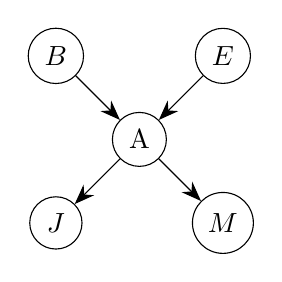
\begin{tikzpicture}[node distance=1.5cm]
      \node[draw,circle] (alarm) {A};
      \node[draw,circle,above left of=alarm] (burglary) {$B$};
      \node[draw,circle,above right of=alarm] (earthquake) {$E$};
      \node[draw,circle,below left of=alarm] (johnCalls) {$J$};
      \node[draw,circle,below right of=alarm] (maryCalls) {$M$};
      \draw[-{Stealth[scale=1.5]}] (burglary) -- (alarm);
      \draw[-{Stealth[scale=1.5]}] (earthquake) -- (alarm);
      \draw[-{Stealth[scale=1.5]}] (alarm) -- (johnCalls);
      \draw[-{Stealth[scale=1.5]}] (alarm) -- (maryCalls);
    \end{tikzpicture}
    \caption{a Bayesian network}
    \label{fig:bn}
  \end{subfigure}
  \begin{subfigure}{0.49\textwidth}
    \centering
    \begin{tikzpicture}[node distance=1.5cm]
      \node[draw,circle] (alarm) {A};
      \node[draw,circle,above left of=alarm] (burglary) {$B$};
      \node[draw,circle,above right of=alarm] (earthquake) {$E$};
      \node[draw,circle,below left of=alarm] (johnCalls) {$J$};
      \node[draw,circle,below right of=alarm] (maryCalls) {$M$};
      \draw[color=color1,ultra thick] (burglary) -- (earthquake);
      \draw[color=color1,ultra thick] (burglary) -- (alarm);
      \draw[color=color1,ultra thick] (earthquake) -- (alarm);
      \draw[color=color2,ultra thick] (alarm) -- (johnCalls);
      \draw[color=color3,ultra thick] (alarm) -- (maryCalls);
    \end{tikzpicture}
    \caption{a Markov network}
    \label{fig:mn}
  \end{subfigure}
%%   \newline
%%   \newline
%%   \begin{subfigure}{\textwidth}
%%     \begin{minipage}{0.57\textwidth}
%%       \centering
%%       \begin{tabular}[t]{lr}
%%         \toprule
%%         $b$ & $\Pr(B = b)$ \\
%%         \midrule
%%         false & 0.999 \\
%%         true & 0.001 \\
%%         \bottomrule
%%       \end{tabular}
%%       \begin{tabular}[t]{lr}
%%         \toprule
%%         $e$ & $\Pr(E = e)$ \\
%%         \midrule
%%         false & 0.998 \\
%%         true & 0.002 \\
%%         \bottomrule
%%       \end{tabular}
%%       \newline
%%       \newline
%%       \begin{tabular}[t]{lllr}
%%         \toprule
%%         $b$ & $e$ & $a$ & $\Pr(A = a \mid B = b, E = e)$ \\
%%         \midrule
%%         false & false & false & 0.999 \\
%%         false & false & true & 0.001 \\
%%         false & true & false & 0.71 \\
%%         false & true & true & 0.29 \\
%%         true & false & false & 0.06 \\
%%         true & false & true & 0.94 \\
%%         true & true & false & 0.05 \\
%%         true & true & true & 0.95 \\
%%         \bottomrule
%%       \end{tabular}
%%     \end{minipage}%
%%     \begin{minipage}{0.43\textwidth}
%%       \centering
%%       \begin{tabular}[t]{llr}
%%         \toprule
%%         $a$ & $j$ & $\Pr(J = j \mid A = a)$ \\
%%         \midrule
%%         false & false & 0.9 \\
%%         false & true & 0.1 \\
%%         true & false & 0.2 \\
%%         true & true & 0.8 \\
%%         \bottomrule
%%       \end{tabular}
%%       \newline
%%       \newline
%%       \begin{tabular}[t]{llr}
%%         \toprule
%%         $a$ & $m$ & $\Pr(M = m \mid A = a)$ \\
%%         \midrule
%%         false & false & 0.9 \\
%%         false & true & 0.1 \\
%%         true & false & 0.2 \\
%%         true & true & 0.8 \\
%%         \bottomrule
%%       \end{tabular}
%%     \end{minipage}
%%     \caption{the CPTs associated with the Bayesian network in \cref{example:bn} and \cref{fig:bn}}
%%     \label{fig:examplecpts}
%%   \end{subfigure}
  \caption{Two PGMs that describe the independence structure of \cref{example:bn}}
\end{figure}

\begin{table}
  \caption{An example CPT for $\Pr(A \mid B, E)$ from \cref{example:bn}}
  \label{table:examplecpt}
  \centering
  \begin{tabular}[t]{lllr}
    \toprule
    $b$ & $e$ & $a$ & $\Pr(A = a \mid B = b, E = e)$ \\
    \midrule
    false & false & false & 0.999 \\
    false & false & true & 0.001 \\
    false & true & false & 0.71 \\
    false & true & true & 0.29 \\
    true & false & false & 0.06 \\
    true & false & true & 0.94 \\
    true & true & false & 0.05 \\
    true & true & true & 0.95 \\
    \bottomrule
  \end{tabular}
\end{table}

The graph of a \emph{Bayesian network} for this example scenario is in \cref{fig:bn}. This (directed acyclic) graph tells us that the joint probability distribution can be factored as
\begin{equation} \label{eq:factorisation}
  \Pr(B, E, A, J, M) = \Pr(B) \times \Pr(E) \times \Pr(A \mid B, E) \times \Pr(J \mid A) \times \Pr(M \mid A),
\end{equation}
i.e., the probability of each random variable is conditioned on its parents in the graph. The factors in \cref{eq:factorisation} can be described using \emph{conditional probability tables} (CPTs). CPTs assign a probability to each combination of values that the random variable and its parents can take---see \cref{table:examplecpt} for an example.

Alternatively, the same probability distribution can be represented as an undirected PGM known as a \emph{Markov network} (or \emph{Markov random field}). The graph of such a network for \cref{example:bn} is in \cref{fig:mn}. Here, instead of CPTs, \emph{potentials} are the building blocks out of which a probability distribution is constructed. A potential is a function from (some subset of) random variables to non-negative real numbers. Potentials are typically defined on the maximal cliques of the network. The edge sets of the three maximal cliques in \cref{fig:mn} are highlighted in different colours. Thus, the full probability distribution can be factorised as
\[
\Pr(B, E, A, J, M) = \frac{1}{Z} \times \psi_1(B, E, A) \times \psi_2(A, J) \times \psi_3(A, M),
\]
where $\psi_1$, $\psi_2$, and $\psi_3$ are potentials, and $Z$ is a normalisation constant known as the \emph{partition function}.

What if we wanted to generalise \cref{example:bn} to support any number of neighbours, all of whom behave identically (i.e., have the same probabilities of calling in all circumstances)? Both Bayesian and Markov networks have been extended for such scenarios: \emph{relational Bayesian networks} \citep{DBLP:conf/uai/Jaeger97} can compactly describe a probability distribution over a relational structure, and \emph{Markov logic networks} (also known as \emph{Markov logic}) \citep{DBLP:journals/ml/RichardsonD06} extend Markov networks with support for first-order logic. The field of learning such representations from data is known as \emph{statistical relational learning} \citep{DBLP:series/synthesis/2016Raedt}. The next section describes relational representations that are based on programming languages instead of graphical models.

\subsection{Probabilistic Programming} \label{sec:probprogramming}

Augmenting a programming language with probabilities is another common way to compactly represent probability distributions. Logic programming languages, in particular, have been frequently used for this purpose. Examples of probabilistic logic programming languages include the independent choice logic \citep{DBLP:journals/ai/Poole97,DBLP:conf/ilp/Poole08}, PRISM \citep{DBLP:conf/ijcai/SatoK97,DBLP:conf/ilp/SatoK08}, BLOG \citep{DBLP:conf/ijcai/MilchMRSOK05}, NP-BLOG \citep{DBLP:conf/uai/CarbonettoKFP05}, ProbLog \citep{DBLP:conf/ijcai/RaedtKT07} and CP-logic \citep{DBLP:journals/tplp/VennekensDB09}. Functional and imperative programming languages have also seen some use, examples of which include BUGS \citep{gilks1994language}, IBAL \citep{DBLP:conf/ijcai/Pfeffer01}, Church \citep{DBLP:conf/uai/GoodmanMRBT08}, and Stan \citep{stan}. More information on probabilistic logic programming, probabilistic programming more generally, and statistical relational artificial intelligence can be found in the work of \citet{DBLP:conf/ilp/2008p}, \citet{DBLP:conf/icse/GordonHNR14}, and \citet{DBLP:series/synthesis/2016Raedt}, respectively.

\begin{lstlisting}[caption=A ProbLog program that computes $\protect{\Pr(B \mid J, M)}$ for the scenario described in \cref{example:bn}, label={lst:problog}]
  neighbour(john).
  neighbour(marry).

  0.001 :: burglary.
  0.002 :: earthquake.

  0.95  :: alarm :- burglary, earthquake.
  0.94  :: alarm :- burglary, \+ earthquake.
  0.29  :: alarm :- \+ burglary, earthquake.
  0.001 :: alarm :- \+ burglary, \+ earthquake.

  0.8   :: calls(X) :- alarm, neighbour(X).
  0.1   :: calls(X) :- \+ alarm, neighbour(X).

  evidence(calls(john)).
  evidence(calls(mary)).
  query(burglary).
\end{lstlisting}

\begin{lstlisting}[escapeinside={(*}{*)},caption=A BLOG program that computes $\protect{\Pr(B \mid J, M)}$ for the scenario described in \cref{example:bn}, label={lst:blog}]
  type Neighbour;
  distinct Neighbour John, Mary;

  random Boolean Burglary   (*$\sim$*) BooleanDistrib(0.001);
  random Boolean Earthquake (*$\sim$*) BooleanDistrib(0.002);

  random Boolean Alarm (*$\sim$*) case[Burglary, Earthquake] in {
    [false, false] -> BooleanDistrib(0.001),
    [false, true]  -> BooleanDistrib(0.29),
    [true, false]  -> BooleanDistrib(0.94),
    [true, true]   -> BooleanDistrib(0.95)
  };

  random Boolean Calls(Neighbour n) (*$\sim$*)
    if Alarm then BooleanDistrib(0.8)
    else BooleanDistrib(0.1);

  obs Calls(John) = true;
  obs Calls(Mary) = true;
  query Burglary;
\end{lstlisting}

\Cref{lst:problog,lst:blog} contain two probabilistic programs that encode the information in \cref{example:bn}. In preparation for \cref{chapter:randomlps}, let us examine the syntax and semantics of ProbLog a bit more closely. ProbLog clauses are exactly like Prolog clauses (see \cref{sec:lp}) but with \verb+p ::+ prepended, for some probability \texttt{p}. Without \verb+::+, the probability associated with the clause is implicitly equal to 1. ProbLog also has keywords \texttt{evidence} and \texttt{query} that are used to define one or more (potentially conditional) probabilities of interest. Reading off the probabilities from \cref{lst:problog}, we can, e.g., compute the probability that John calls as
\begin{align*}
  \Pr(j) &= \Pr(b)\Pr(e)\Pr(a \mid b, e)\Pr(j \mid a) \\
  &+ \Pr(b)\Pr(e)\Pr(\neg a \mid b, e)\Pr(j \mid \neg a) \\
  &+ \cdots \\
  &+ \Pr(\neg b)\Pr(\neg e)\Pr(\neg a \mid \neg b, \neg e)\Pr(j \mid \neg a) \\
  &= 0.001 \times 0.002 \times 0.95 \times 0.8 + \cdots \\
  &\approx 0.102.
\end{align*}
More formally, the probability of a query is the sum of the probabilities of the models of the query (c.f. WMC).

\section{Knowledge Compilation and Representation} \label{sec:kc}
% Probabilistic SDDs \citep{DBLP:conf/kr/KisaBCD14} extend SDDs with probability labels on edges.

Many WMC algorithms rely on knowledge compilation, i.e., compilation of the structure of the initial representation into a form that allows one to perform various operations and answer queries of interest in time polynomial in the size of the compiled representation.

Traditionally, the initial representation is a propositional formula.

Many such representations have been proposed \citep{DBLP:journals/jair/DarwicheM02}.

Amongst them, the ones that are used in probabilistic inference include (reduced ordered) \emph{binary decision diagrams} (BDDs) \citep{DBLP:journals/tc/Bryant86}, \emph{deterministic decomposable negation normal form} (d-DNNF) \citep{DBLP:journals/jancl/Darwiche01}, and \emph{sentential decision diagrams} (SDDs) \citep{DBLP:conf/ijcai/Darwiche11}---some of them are pictured in \cref{fig:kc}.

\begin{definition}
  A propositional formula $\phi$ is in \emph{negation normal form} (NNF) if
  \begin{itemize}
  \item the only operators in $\phi$ are $\neg$, $\lor$, and $\land$,
  \item and $\neg$ is only applied to directly to variables.
  \end{itemize}
\end{definition}

\begin{example}
  Formula $\neg(C \Rightarrow (\neg A \land B))$ can be transformed into NNF as follows:
  \[
  \neg(C \Rightarrow (\neg A \land B)) \equiv \neg(\neg C \lor (\neg A \land B)) \equiv C \land (A \lor \neg B)
  \]
  using the definition of $\Rightarrow$ and De Morgan's laws.
\end{example}

\begin{definition}
  The d-DNNF adds decomposability and determinism to the NNF. \emph{Decomposability} requires that, for every conjunction $\bigwedge_{i=1}^n \phi_i$, conjuncts $\phi_i$ and $\phi_j$ have no variables in common for all $i \ne j$ \citep{DBLP:conf/ijcai/Darwiche99,DBLP:journals/jacm/Darwiche01}. \emph{Determinism} requires that, for every disjunction $\bigvee_{i=1}^n \phi_i$, disjuncts $\phi_i$ and $\phi_j$ contradict each other (i.e., $\phi_i \land \phi_j \equiv \bot$) for all $i \ne j$ \citep{DBLP:journals/jancl/Darwiche01}.
\end{definition}

\begin{example}
  Formula $(A \lor \neg B) \land (A \lor C)$ is neither decomposable nor deterministic. It is not decomposable because $\{\, A, B \,\} \cap \{\, A, C \,\} = \{\, A \,\} \ne \emptyset$. It is not deterministic because, e.g., $A \land \neg B \not\equiv \bot$.
\end{example}

\begin{example} \label{example:ddnnf1}
  Formula $C \land (A \lor \neg B)$ is decomposable but not deterministic. It is decomposable because $\{\, C \,\} \cap \{\, A, B \,\} = \emptyset$. It is not deterministic because $A \land \neg B \not\equiv \bot$.
\end{example}

\begin{example}
  Formula $B \land C \land [\neg B \lor (A \land B)]$ is deterministic but not decomposable. It is deterministic because $\neg B \land A \land B \equiv \bot$. It is not decomposable because $\{\, B \,\} \cap \{\, A, B \,\} = \{\, B \,\} \ne \emptyset$.
\end{example}

\begin{example} \label{example:ddnnf2}
  Formula $C \land [\neg B \lor (A \land B)]$ is decomposable and deterministic. It is decomposable because $\{\, C \,\} \cap \{\, A, B \,\} = \emptyset$, and $\{\, A \,\} \cap \{\, B \,\} = \emptyset$. It is deterministic because $\neg B \land A \land B \equiv \bot$.
\end{example}

\begin{figure}
  \centering
  \begin{subfigure}{0.32\textwidth}
    \centering
    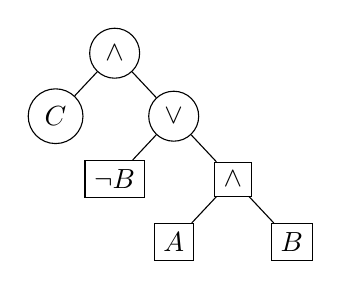
\begin{tikzpicture}[level distance=0.8cm] % C \land [\neg B \lor (A \land B)]
      \node[draw,circle] {$\land$}
      child {node[draw,circle] {$C$}}
      child {node[draw,circle] {$\lor$}
        child {node[draw,rectangle] {$\neg B$}}
        child {node[draw,rectangle] {$\land$}
          child {node[draw,rectangle] {$A$}}
          child {node[draw,rectangle] {$B$}}
        }
      };
    \end{tikzpicture}
    \caption{d-DNNF}
    \label{fig:ddnnf}
  \end{subfigure}
  \begin{subfigure}{0.32\textwidth}
    \centering
    \begin{tikzpicture}[level distance=0.8cm]
      \tikzset{
        mysplit/.style={
          draw,
          rectangle,
          rectangle split,
          rectangle split horizontal,
          rectangle split parts=2
        }
      }
      \node[draw,circle] {$1$}
      child {node[mysplit] (bullet) {
          \nodepart{one} $\neg A$
          \nodepart{two}
        }
        child {node[draw,circle] (3) {$3$} edge from parent[draw=none]
          child {node[mysplit] {
              \nodepart{one} $\neg B$
              \nodepart{two} $C$
            }
          }
          child {node[mysplit] {
              \nodepart{one} $B$
              \nodepart{two} $\bot$
            }
          }
        }
      }
      child {node[mysplit] {
          \nodepart{one} $A$
          \nodepart{two} $C$
        }};
      \draw[*-] let \p1 = (bullet.two), \p2 = (bullet.center) in ({\x1 + 2.5},{\y2 + 2}) -- (3);
    \end{tikzpicture}
    \caption{SDD}
    \label{fig:sdd}
  \end{subfigure}
  \begin{subfigure}{0.32\textwidth}
    \centering
    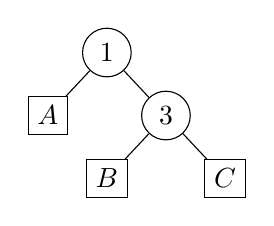
\begin{tikzpicture}[level distance=0.8cm]
      \node[draw,circle] {$1$}
      child {node[draw,rectangle] {$A$}}
      child {node[draw,circle] {$3$}
        child {node[draw,rectangle] {$B$}}
        child {node[draw,rectangle] {$C$}}
      };
    \end{tikzpicture}
    \caption{vtree}
    \label{fig:vtree}
  \end{subfigure}
  \caption{A d-DNNF and an SDD representation of $C \land (A \lor \neg B)$, together with the corresponding vtree. The numbers 1 and 3 come from the in-order traversal of the vtree and visually connect subtrees of both the SDD and the vtree.}
  \label{fig:kc}
\end{figure}

Note that the formulas in \cref{example:ddnnf1,example:ddnnf2} are equivalent, and the latter is also pictured in \cref{fig:ddnnf}.

Next, to define SDDs, we first need to define vtrees.

\begin{definition}[\citep{DBLP:conf/aaai/PipatsrisawatD08}]
  A \emph{vtree} for a set of variables $X$ is a full binary tree $T$ with a bijection between $X$ and the leaves of $T$.
\end{definition}

Let $\langle\cdot\rangle$ denote the function that maps an SDD to the propositional formula that it represents.

\begin{definition}[\citep{DBLP:conf/ijcai/Darwiche11}]
  Let $V$ be a vtree for a set of variables $X$. Then $S$ is an \emph{SDD} that respects $V$ if one of the following is true:
  \begin{itemize}
  \item $S = \bot$ ($\langle \bot \rangle \coloneqq \bot$);
  \item $S = \top$ ($\langle \top \rangle \coloneqq \top$);
  \item $S = x$, or $S = \neg x$, where $x \in X$ is the variable bijectively associated with the \emph{only} node of $V$ ($\langle x \rangle \coloneqq x$, and $\langle \neg x \rangle \coloneqq \neg x$);
  \item $S = \{\, (p_i, s_i) \mid i = 1, \dots, n \,\}$ for some $n \ge 1$, where \emph{primes} $\{\,p_i\,\}_{i=1}^n$ and \emph{subs} $\{\,s_i\,\}_{i=1}^n$ are SDDs such that:
    \begin{itemize}
    \item $V$ has more than one node,
    \item each $p_i$ respects the left subtree of $V$,
    \item each $s_i$ respects the right subtree fo $V$.
    \item the primes form a \emph{partition}, i.e.:
      \begin{itemize}
      \item $\langle p_i \rangle \not\equiv \bot$ for all $i = 1, \dots, n$ (i.e., the primes are \emph{consistent}),
      \item $\langle p_i \rangle \land \langle p_j \rangle \equiv \bot$ for all $i \ne j$ (i.e., the primes are \emph{mutually exclusive}),
      \item and $\bigvee_{i=1}^n \langle p_i \rangle \equiv \top$
      \end{itemize}
    \end{itemize}
    (then $\langle S \rangle \coloneqq \bigvee_{i=1}^n \langle p_i \rangle \land \langle s_i \rangle$).
  \end{itemize}
\end{definition}

\begin{example}
  Let $S = \{\, (A, C), (\neg A, \{\, (\neg B, C), (B, \bot) \,\}) \,\}$. Then $S$ (as pictured in \cref{fig:sdd}) is an SDD representation of $C \land (A \lor \neg B)$ that respects the vtree in \cref{fig:vtree}. Indeed,
  \begin{align*}
    \langle S \rangle &= (A \land C) \lor (\neg A \land [(\neg B \land C) \lor (B \land \bot)]) \\
    &\equiv (A \land C) \lor (\neg A \land \neg B \land C) \\
    &\equiv C \land (A \lor [\neg A \land \neg B]) \\
    &\equiv C \land ([A \lor \neg A] \land [A \lor \neg B]) \\
    &\equiv C \land (\top \land [A \lor \neg B]) \\
    &\equiv C \land (A \lor \neg B).
  \end{align*}
\end{example}

A BDD is similar to a decision tree that ends with either one or zero but generalised to a directed acyclic graph.

Both d-DNNF and SDD are normal forms for propositional formulae that satisfy certain properties.

\begin{figure}
  \centering
  \begin{subfigure}{0.18\textwidth}
    \centering
    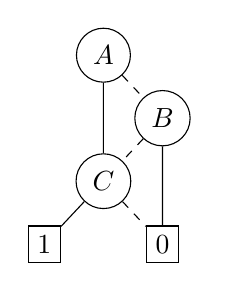
\begin{tikzpicture}[level distance=0.8cm]
      \node[draw,circle] (A) {$A$}
      child {edge from parent[draw=none]}
      child {node[draw,circle] (B) {$B$} edge from parent[dashed]
        child {node[draw,circle,solid] (C) {$C$} edge from parent[dashed]
          child {node[draw,rectangle,solid] {$1$} edge from parent[solid]}
          child {node[draw,rectangle,solid] (0) {$0$}}
        }
        child {edge from parent[draw=none]}
      };
      \draw (A) -- (C);
      \draw (B) -- (0);
    \end{tikzpicture}
    \caption{BDD}
    \label{fig:bdd}
  \end{subfigure}
  \begin{subfigure}{0.20\textwidth}
    \centering
    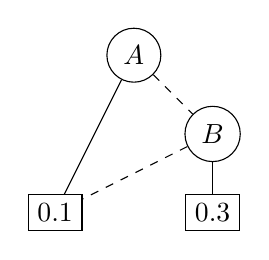
\begin{tikzpicture}
      \node[circle,draw] (x) at (0, 0) {$A$};
      \node[circle,draw] (y) at (1, -1) {$B$};
      \node[draw] (a) at (-1, -2) {0.1};
      \node[draw] (b) at (1, -2) {0.3};
      \draw[dashed] (x) -- (y);
      \draw (x) -- (a);
      \draw[dashed] (y) -- (a);
      \draw (y) -- (b);
    \end{tikzpicture}
    \caption{ADD}
    \label{fig:add}
  \end{subfigure} % TODO: could redraw the third diagram to be more like the others
\end{figure}

BDDs are a strict subset of SDDs that are a strict subset of d-DNNF \citep{DBLP:conf/ijcai/Darwiche11}.

Similarly to how BDDs represent Boolean functions, ADDs represent pseudo-Boolean functions, i.e., while (non-trivial) BDDs always have two sinks marked with one and zero, ADDs can have any number of sinks that contain, typically, real numbers \citep{DBLP:journals/fmsd/BaharFGHMPS97}.

ADDs have been extended to represent the additive and multiplicative structure in sink values more compactly \citep{DBLP:conf/ijcai/SannerM05} and to support first-order logic \citep{DBLP:journals/ai/SannerB09} and continuous variables \citep{DBLP:conf/uai/SannerDB11}.

ADDs have been used to represent the value functions of Markov decision processes \citep{DBLP:conf/uai/HoeySHB99} and probabilities in PGMs \citep{DBLP:conf/ijcai/ChaviraD07,DBLP:conf/uai/GogateD11}.

\begin{itemize}
\item maybe add a vtree for the SDD from the slides? I think the vtree is wrong...
\item have an example of an SDD in its set-of-sets-of...of literals and top/bot.
\item say: These formulas are often interpreted as trees or DAGs.
\item TODO: add info from the random slides, Chapter 5, and the full KR paper. But how much?
\item explain why the focus is on representations of propositional formulas and pseudo-Boolean functions
\item Boolean and Pseudo-Boolean Functions
\item NNF and how d-DNNF restricts that
\item A graphical representation of the ADD from ??. Sinks are represented as rectangles and other nodes as circles. The labels of nodes are written directly on them. An edge $e$ is dashed if $\epsilon(e) = 0$ and solid otherwise.
\item advertise \citep{DBLP:journals/jair/DarwicheM02} as a description of many normal forms and representations
\end{itemize}

\section{Applications}

of WMC?

copy info from my year 2 report

\begin{itemize}
\item Statistical Relational Learning
\item Neuro-Symbolic Artificial Intelligence
\item Natural Language Processing
\item Robotics
\end{itemize}
 % 11-45 pages (27 on average)
\chapter{Generating Random WMC Instances} \label{chapter:comparison}

\section{Introduction}

% WMC
Weighted model counting (\textsf{WMC})---a weighted generalisation of
propositional model counting
($\#\SAT{}$) \citep{DBLP:journals/ai/ChaviraD08}---has emerged as a powerful
computational framework for problems in a variety of domains. In particular,
\textsf{WMC} has been used to perform probabilistic inference for graphical
models such as Bayesian networks and Markov random
fields \citep{DBLP:conf/ecai/BartKLM16,DBLP:conf/ijcai/ChaviraD05,DBLP:conf/sat/ChaviraD06,DBLP:conf/kr/Darwiche02,DBLP:conf/aaai/SangBK05},
probabilistic programs \citep{DBLP:journals/pacmpl/HoltzenBM20}, and
probabilistic logic programs \citep{DBLP:journals/tplp/FierensBRSGTJR15}. More
recently, \textsf{WMC} was used in the context of neural-symbolic artificial
intelligence as well \citep{DBLP:conf/icml/XuZFLB18}. Extensions of \textsf{WMC}
add support for continuous variables \citep{DBLP:conf/ijcai/BellePB15}, infinite
domains \citep{DBLP:conf/aaai/Belle17}, and first-order
logic \citep{DBLP:conf/ijcai/BroeckTMDR11,DBLP:journals/cacm/GogateD16} and
generalise the definition to support arbitrary pseudo-Boolean functions instead
of clauses \citep{DBLP:conf/sat/DilkasB21}.
Exact \textsf{WMC} algorithms can be broadly classified as based on
search \citep{DBLP:conf/sat/SangBBKP04,DBLP:conf/ijcai/SharmaRSM19}, knowledge
compilation \citep{DBLP:conf/ecai/Darwiche04,DBLP:conf/ijcai/LagniezM17,DBLP:conf/ijcai/OztokD15}, and
dynamic programming \citep{DBLP:conf/aaai/DudekPV20,DBLP:conf/cp/DudekPV20}. Other alternatives include approximate \citep{DBLP:conf/aaai/RenkensKBR14} and parallel algorithms \citep{DBLP:conf/pgm/DalLL18,DBLP:conf/esa/FichteHWZ18}, hybrid approaches \citep{DBLP:conf/sat/HecherTW20}, quantum computing \citep{DBLP:conf/ecai/Riguzzi20}, and reduction to model counting \citep{DBLP:conf/ijcai/ChakrabortyFMV15}.

% motivation for the problem
Recent papers that include experimental comparisons of \textsf{WMC}
algorithms show many of them performing very similarly
overall \citep{DBLP:conf/aaai/DudekPV20,DBLP:conf/cp/DudekPV20} but with
overwhelming differences when run on specific subsets of
data \citep{DBLP:conf/uai/DilkasB21,DBLP:conf/sat/DilkasB21,DBLP:conf/ijcai/LagniezM17}.
Examples of such segregating data sets include bipartite Bayesian networks by
\citet{DBLP:conf/aaai/SangBK05} and
relational Bayesian networks by
\citet{DBLP:journals/ijar/ChaviraDJ06}
that encode reachability in graphs under node deletion. So far, such performance
differences remain unexplained. However, knowledge about the nature of these
differences can inform our choices and aid in further algorithmic developments.
Moreover, identifying performance predictors of algorithms is often an important
step in developing a portfolio approach to the
problem \citep{DBLP:journals/jair/XuHHL08}. Lastly, if new algorithms are always
tested on the same set of benchmarks, eventually they may become somewhat fitted
to the particular characteristics of those instances, leading to algorithms that
may perform worse when run on new types of
data \citep{DBLP:conf/cec/HossainALA10}.

% related work on SAT
Both theoretical and experimental analysis of \SAT{} (and, to a lesser extent,
$\#\SAT{}$) algorithms on random instances is a rich area of research spanning
almost forty years. Variations of some of the first random models ever
proposed \citep{DBLP:journals/dam/FrancoP83,DBLP:journals/siamcomp/PurdomB83}
continue to be instrumental up to this day for, e.g., establishing the location
of the threshold between satisfiable and unsatisfiable
instances \citep{DBLP:conf/focs/AchlioptasM02} and efficiently approximating
$\#\SAT{}$ \citep{DBLP:conf/icalp/GalanisG0Y20}. Other random models consider
non-uniform variable frequencies \citep{DBLP:conf/ijcai/AnsoteguiBL09}, fixing
the number of times each variable occurs both positively and
negatively \citep{DBLP:journals/cpc/Coja-OghlanW18}, and adding other constraints
such as cardinality and `exclusive or' \citep{DBLP:conf/ijcai/PoteJM19}. In
contrast, only one \textsf{WMC} algorithm so far has been analysed using random
instances \citep{DBLP:conf/sat/SangBBKP04,DBLP:conf/sat/SangBK05}. Similarly,
while there is a recent attempt \citep{DBLP:conf/cp/DilkasB20} to compare
\textsf{WMC} algorithms on random instances of a particular application of
\textsf{WMC} (i.e., probabilistic logic programs), it fails to discern any
meaningful differences among the algorithms. The goal of this paper is to
explain some of the differences between \textsf{WMC} algorithms via an
experimental study that uses random instances.

% parameters for SAT
Experimental work investigating how \SAT{} algorithms behave on random
instances is typically centred around parameters that describe each instance
independently of its size. The most well-known parameter is the ratio of clauses
to variables (i.e., \emph{(clause) density}). Early work in the area
showed random 3-\SAT{} instances to be at their hardest when density is
around 4.25 \citep{DBLP:conf/aaai/MitchellSL92}. Later work revealed that the
interaction between density and empirical hardness is much more
solver-dependent \citep{DBLP:journals/constraints/CoarfaDASV03}. Many other
parameters such as heterogeneity, locality, and modularity have emerged from
attempts to generate random instances similar to industry benchmarks for
\SAT{} \citep{DBLP:conf/ijcai/AnsoteguiBL09,DBLP:conf/tacas/BlasiusFS19,DBLP:journals/ai/Giraldez-CruL16,DBLP:conf/ijcai/Giraldez-CruL17}.

% parameters for WMC
What parameter(s) are most appropriate to study \textsf{WMC}? Theoretical upper
bounds on the performance of various \textsf{WMC} algorithms typically include a
factor exponential in the primal treewidth of the input formula (or a closely
related
notion) \citep{DBLP:journals/jair/BacchusDP09,DBLP:journals/jacm/Darwiche01,DBLP:conf/ecai/Darwiche04,DBLP:conf/sat/SangBBKP04}.
However---as we show in \cref{sec:model}---instances generated by a standard
random model for $k$-CNF formulas fail to exhibit enough variance in primal
treewidth for us to infer its effect on the behaviour of the algorithms.
Therefore, we present an extension of this model with a parameter that
influences primal treewidth. The performance of \textsf{WMC} algorithms that use
data structures called \emph{algebraic decision diagrams}
(ADDs) \citep{DBLP:journals/fmsd/BaharFGHMPS97} is also known to depend on the
numerical values of
weights \citep{DBLP:conf/aaai/DudekPV20,DBLP:conf/cp/DudekPV20}. Thus, our random
model also includes two parameters that control redundancies in these values.
We also
investigate the effect of redundant weight values (e.g., having weights set to
zero and one or having the same weight repeat many times) on the running times
of the algorithms.

In addition to introducing a new random model for \textsf{WMC} instances, the
contributions of this paper include several key experimental findings about the
behaviour of \textsf{WMC} algorithms---namely,
\textsc{c2d}\footnote{\url{http://reasoning.cs.ucla.edu/c2d/}} \citep{DBLP:conf/ecai/Darwiche04},
\textsc{Cachet}\footnote{\url{https://cs.rochester.edu/u/kautz/Cachet/}} \citep{DBLP:conf/sat/SangBBKP04},
\textsc{d4}\footnote{\url{https://www.cril.univ-artois.fr/KC/d4.html}} \citep{DBLP:conf/ijcai/LagniezM17},
\textsc{DPMC}\footnote{\url{https://github.com/vardigroup/dpmc}} \citep{DBLP:conf/cp/DudekPV20},
and
\textsc{miniC2D}\footnote{\url{http://reasoning.cs.ucla.edu/minic2d/}} \citep{DBLP:conf/ijcai/OztokD15}---on
random instances. First, we show that the easy-hard-easy pattern with respect to
(w.r.t.) density is different for dynamic programming algorithms than it is for
all other algorithms. Second, we present statistical evidence that all the
algorithms scale exponentially w.r.t.\ primal treewidth and estimate how the
base of that exponential changes w.r.t.\ density. Third, we show how the
performance of ADD-based algorithms gradually improves w.r.t the proportion of
weights that have repeating values and sharply improves w.r.t.\ the proportion
of weights set to zero and one.

% 1. Other parameters include structural entropy
% \cite{DBLP:journals/access/LinWN21}, the proportion of clauses that have at
% most one negative literal has also been suggested as a parameter of
% interest~\cite{DBLP:journals/amai/MaarenN05}.
% 2. Maybe somewhere: relationship between primal treewidth and modularity
% 3. Just like one might choose a different propositional satisfiability
% (\SAT{}) solver based on information about the problem instance at hand (e.g.,
% `is the instance known to be satisfiable?', `was it randomly generated?', `is
% it an industrial instance?')~\cite{DBLP:journals/jair/XuHHL08},
% 4. It was also observed that replacing real numbers with addition and
% multiplication with an arbitrary commutative semiring allows \textsf{WMC} to
% subsume a variety of other problems such as most probable explanation,
% shortest path, and gradient
% computations~\cite{DBLP:journals/ijar/BelleR20,DBLP:journals/japll/KimmigBR17}.
% 5. Having these parameters in the model allows us to look not just at the
% effects of density or primal treewidth on the running times of \textsf{WMC}
% algorithms but also at the interaction between these two parameters of
% interest.

\section{Preliminaries}

% \footnote{Also known by many other names such as Gaifman, (variable)
% interaction, and variable incidence graph.}

By \emph{variable}, we always mean a Boolean variable. A \emph{literal} is
either a variable (say, $v$) or its negation (denoted $\neg v$), respectively
called \emph{positive} and \emph{negative} literal. A \emph{clause} is a
disjunction of literals. A \emph{formula} is any well-formed expression
consisting of variables, negation, conjunction, and disjunction. A formula is in
\emph{conjunctive normal form} (CNF) if it is a conjunction of clauses, and it
is in $k$-CNF if every clause has exactly $k$ literals. While we use the
set-theoretic notation for CNF formulas (e.g., writing $c \in \phi$ to mean that
clause $c$ is one of the clauses in formula $\phi$), duplicate clauses are still
allowed. The \emph{primal graph} of a CNF formula is a graph that has a node for
every variable, and there is an edge between two variables if they coappear in
some clause. The \emph{treewidth} of a graph $G$ measures how similar $G$
is to a tree and is defined as the smallest \emph{width} of any \emph{tree
  decomposition} of $G$ \citep{DBLP:journals/jct/RobertsonS84}. The \emph{primal
  treewidth} of a formula is the treewidth of its primal graph.

Given a CNF formula $\phi$, \SAT{} is a decision problem that asks whether there
exists a way to assign values to all variables in $\phi$ such that $\phi$
evaluates to true. Such a formula is said to be \emph{satisfiable}; otherwise,
it is \emph{unsatisfiable}. $\#\SAT{}$ is a problem that asks to count the
number of such assignments. \textsf{WMC} extends $\#\SAT{}$ with a weight
function on literals and asks to compute the sum of the weights of the models of
the given formula, where the weight of a model is the product of the weights of
the literals in it \citep{DBLP:journals/ai/ChaviraD08}. For example, the
\textsf{WMC} of the formula $x \lor y$ with a weight function $w\colon \{\,x, y,
\neg x, \neg y\,\} \to \mathbb{R}_{\ge 0}$ defined as $w(x) = 0.3$, $w(y) = 0.2$,
$w(\neg x) = 0.7$, $w(\neg y) = 0.8$ is $w(x)w(y)+w(x)w(\neg y)+w(\neg x)w(y) =
0.3 \times 0.2 + 0.3 \times 0.8 + 0.7 \times 0.2 = 0.44$.

\section{Background on \textsf{\textmd{WMC}} Algorithms}\label{sec:background}

In this section, we briefly review the three major approaches to \textsf{WMC}---search, knowledge compilation, and dynamic programming---and their corresponding algorithms. The main search-based \textsf{WMC} algorithm \textsc{Cachet} \citep{DBLP:conf/sat/SangBBKP04} is based on a conflict-driven clause learning \SAT{} solver \citep{DBLP:conf/dac/MoskewiczMZZM01}, which is then extended with a component caching scheme and adapted to counting.

\emph{Knowledge compilation} refers to transformations of propositional formulas
into more restrictive formats that make various operations (such as model
counting) tractable in the size of the representation
\citep{DBLP:journals/jair/DarwicheM02}.
\textsc{c2d} \citep{DBLP:conf/ecai/Darwiche04},
\textsc{d4} \citep{DBLP:conf/ijcai/LagniezM17}, and
\textsc{miniC2D} \citep{DBLP:conf/ijcai/OztokD15}
are all algorithms of this type. \textsc{c2d} compiles to deterministic
decomposable negation normal form
(d-DNNF) \citep{DBLP:journals/jancl/Darwiche01}. Similarly, \textsc{d4} compiles
to decision-DNNF (also known as decomposable decision
graphs) \citep{DBLP:conf/aaai/FargierM06}. The only difference between d-DNNF and
decision-DNNF is that decision-DNNF has if-then-else constructions instead of
disjunctions \citep{DBLP:conf/ijcai/LagniezM17}. Finally,
\textsc{miniC2D} compiles to decision-SDDs---a
subset of sentential decision diagrams (SDDs) that form a subset of
d-DNNF \citep{DBLP:conf/ijcai/Darwiche11}.

All of the algorithms mentioned above execute in exactly the same way regardless of whether computing \textsf{WMC} or $\#\SAT{}$. Two recent \textsf{WMC} algorithms instead use data structures whose size (and thus the runtime of the algorithm) depends on the numerical values of weights. These data structures are representations of \emph{pseudo-Boolean functions}, i.e., functions of the form $f\colon 2^X \to \mathbb{R}_{\ge 0}$, where $X$ is a set, and $2^X$ denotes its powerset. \textsc{ADDMC} is the first such algorithm \citep{DBLP:conf/aaai/DudekPV20}. It uses ADDs to represent pseudo-Boolean functions, combining and simplifying them in a bottom-up dynamic programming fashion. Since the size of an ADD for $f$ depends on the cardinality of the range of $f$ \citep{DBLP:journals/fmsd/BaharFGHMPS97}, the performance of the algorithm is sensitive to the numerical values of weights, e.g., to how frequently they repeat. \textsc{DPMC} extends \textsc{ADDMC} in two ways \citep{DBLP:conf/cp/DudekPV20}. First, \textsc{DPMC} allows for the order and nesting of operations on ADDs to be determined from an approximately-minimal-width tree decomposition rather than by heuristics.\footnote{There is also a recent line of work in using tree decompositions to guide the heuristics of search-based model counters \citep{DBLP:conf/cp/KorhonenJ21}.} Second, tensors are offered as an alternative to ADDs.

In all known parameterised complexities of \textsf{WMC} algorithms, the
exponential factor is a function of primal treewidth or a closely related
parameter. Interestingly, \textsc{c2d} is specifically designed to handle high
primal treewidth (which the author refers to as
\emph{connectivity} \citep{DBLP:conf/ijcai/Darwiche99}) and improves upon an
earlier algorithm that has $\mathcal{O}(mw2^w)$ time complexity, where $m$ is
the number of clauses, and $w$ is the width of the decomposition tree which is
known to be at most primal
treewidth \citep{DBLP:journals/jacm/Darwiche01,DBLP:conf/ecai/Darwiche04}. While
the complexity of \textsc{Cachet} was not analysed directly, the algorithm is
based on component caching which is known to have a
$2^{\mathcal{O}(w)}n^{\mathcal{O}(1)}$ time complexity, where $n$ is the number
of variables, and $w$ is the branchwidth of the underlying
hypergraph \citep{DBLP:journals/jair/BacchusDP09,DBLP:conf/sat/SangBBKP04}, which
is known to be within a constant factor of primal
treewidth \citep{DBLP:journals/jct/RobertsonS91}. Similarly, the complexity of
\textsf{DPMC} is not described in the paper, although the authors define a
notion of width $w$ that is at most primal treewidth plus one and estimate the
running time of the (execution part of the) algorithm to be proportional to
$2^w$ \citep{DBLP:conf/cp/DudekPV20}.

\section{Random $k$-CNF Formulas with Varying Primal
  Treewidth}\label{sec:model}

\paragraph{Notation.}
For any graph $G$, we write $\mathcal{V}(G)$ for its set of nodes and
$\mathcal{E}(G)$ for its set of edges. Let $S$ be a finite set. We write
$\mathcal{U}S$ for the discrete uniform probability distribution on $S$. We
represent any other probability distribution as a pair $(S, p)$ where $p\colon S
\to [0, 1]$ is a probability mass function. For any probability distribution
$\mathcal{P}$, we write $x \leftlsquigarrow \mathcal{P}$ to denote the act of
sampling $x$ from $\mathcal{P}$. For instance, $x \leftlsquigarrow (\{\, 1, 2 \,\}, \{\, 1 \mapsto 0.1, 2 \mapsto 0.9 \,\})$ means that $x$ becomes equal to $1$ with probability $0.1$ or to $2$ with probability $0.9$.

Our random model is based on the following parameters:
\begin{itemize}
\item the number of variables $\nu \in \mathbb{N}^+$,
\item density $\mu \in \mathbb{R}_{>0}$,
\item clause width $\kappa \in \mathbb{N}^+$ (for $k$-CNF formulas, $\kappa =
  k$),
\item a parameter $\rho \in [0, 1]$ that influences the primal treewidth of
  the formula,
\item the proportion $\delta \in [0, 1]$ of variables $x$ such that $w(x) = 1$
  and $w(\neg x) = 0$ or $w(x) = 0$ and $w(\neg x) = 1$,
\item and the proportion $\epsilon \in [0, 1-\delta]$ of variables $x$ such that
  $w(x) = w(\neg x) = 0.5$.
\end{itemize}
The first three parameters are the standard parameters used to generate random
$k$-CNF formulas with $\nu\mu$ clauses (up to rounding). We expect to observe
(possibly different) values of $\mu$ that maximize the running time of each
algorithm for fixed values of $\nu$ and $\kappa$. Parameters $\delta$ and
$\epsilon$ control the numerical values of weights and are part of the model
because the running time of \textsc{DPMC} \citep{DBLP:conf/cp/DudekPV20}---and
other algorithms based on ADDs---depends on these values. Weights such as zero
and one are particularly `simplifying' because they are respectively the
additive and multiplicative identities. Having them propagate through the
algorithm reduces the size of many ADDs used by \textsc{DPMC}, making the
algorithm more efficient. Including many copies of the same weight (e.g., 0.5)
can similarly simplify ADDs as well. Other \textsf{WMC} algorithms are
indifferent to the numerical values of weights.

\begin{algorithm}[t]
  \caption{Generating a random formula.}\label{alg:random}
  \SetKwData{kcnf}{kcnf}
  \SetKwFunction{NewVariable}{NewVariable}
  \SetKwProg{Fn}{Function}{:}{}
  \KwIn{$\nu,\kappa \in \mathbb{N}^+$ such that $\kappa < \nu$, $\mu \in
    \mathbb{R}_{>0}$, $\rho \in [0, 1]$.}
  \KwOut{A $k$-CNF formula $\phi$.}
  $\phi \gets \text{empty CNF formula}$\;
  $G \gets \text{empty graph}$\;
  \For{$i \gets 1$ \KwTo $\lfloor \nu\mu \rfloor$}{
    $X \gets \emptyset$\;
    \For{$j \gets 1$ \KwTo $\kappa$}{
      $x \gets \NewVariable{$X$, $G$}$\;
      $\mathcal{V}(G) \gets \mathcal{V}(G) \cup \{\, x \,\}$\;\label{line:7}
      $\mathcal{E}(G) \gets \mathcal{E}(G) \cup \{\, \{\,x, y\,\} \mid y \in X
      \,\}$\;\label{line:8}
      $X \gets X \cup \{\, x \,\}$\;\label{line:9}
    }
    $\phi \gets \phi \cup \{\, l \leftlsquigarrow \mathcal{U}\{\, x, \neg x \,\}
    \mid x \in X \,\}$\;\label{line:construct_clause}
  }
  \Return{$\phi$}\;
  \Fn{\NewVariable{$X$, $G$}}{
    $N \gets \{\, e \in \mathcal{E}(G) \mid |e \cap X| = 1
    \,\}$\;\label{line:13}
    \If{$N = \emptyset$}{
      \Return{$x \leftlsquigarrow \mathcal{U}(\{\, x_1, x_2, \dots, x_\nu \,\}
        \setminus X)$}\;
    }
    \nosemic\Return{$x \leftlsquigarrow \left(\{\, x_1, x_2, \dots, x_\nu \,\}
        \setminus X,\vphantom{\frac{|\{\, z \in X \mid \{\,y, z\,\} \in
            \mathcal{E}(G) \,\}|}{|N|}}\right.$}\;
      \pushline\dosemic$\left. y \mapsto \frac{1 - \rho}{\nu - |X|} +
        \rho\frac{|\{\, z \in X \mid \{\,y, z\,\} \in \mathcal{E}(G)
          \,\}|}{|N|}\right)$\; \label{line:return}
  }
\end{algorithm}

The process behind generating random $k$-CNF formulas is summarized as
\cref{alg:random}. For the rest of this section, let $x_1, x_2, \dots, x_\nu$ be
the variables of the formula under construction. We simultaneously construct
both formula $\phi$ and its primal graph $G$.\footnote{The idea to directly take
  the primal graph into consideration while generating the formula is new---cf.
  random \SAT{} instance generators based on, e.g., adversarial evolution
  \citep{DBLP:conf/cec/HossainALA10} and community structure
  \citep{DBLP:journals/ai/Giraldez-CruL16}.} Each iteration of the first for-loop
adds a clause to $\phi$. This is done by constructing a set $X$ of variables to
be included in the clause, and then randomly adding either $x$ or $\neg x$ to
the clause for each $x \in X$ on \cref{line:construct_clause}. Function
\texttt{NewVariable} randomly selects each new variable $x$, and
\cref{line:7,line:8,line:9} add $x$ to the graph and the formula while also
adding edges between $x$ and all the other variables in the clause. To select
each variable, \cref{line:13} defines set $N$ to contain all edges with exactly
one endpoint in $X$. The edges that will be added to $G$ by \cref{line:8} will
form a subset of $N$. If $N = \emptyset$, we select the variable uniformly at
random (u.a.r.) from all viable candidates. Otherwise, $\rho$ determines how
much we bias the uniform distribution towards variables that would introduce the
smallest number of new edges to $G$.

When $\rho=0$, \cref{alg:random} reduces to what has become the standard random
model for $k$-CNF formulas. Equivalently to \citet{DBLP:journals/dam/FrancoP83},
we independently sample a fixed number of clauses, each clause has no duplicate
variables, and each variable becomes either a positive or a negative literal
with equal probabilities. At the other extreme, when $\rho = 1$, the first
variable of a clause is still chosen u.a.r., but all other variables are chosen
from those that already coappear in a clause (if possible). The probability that
a variable is selected to be included in a clause scales linearly w.r.t.\ the
proportion of edges in $N$ that would be repeatedly added to $G$ if the variable
$y$ was added to the clause. This is an arbitrary choice (which appears to work
well, see \cref{sec:remarks}) although alternatives (e.g., exponential scaling)
could be considered. As long as $\rho < 1$, every $k$-CNF formula retains a
positive probability of being generated by the algorithm.

To transform the generated formula into a \textsf{WMC} instance, we need
to define weights on literals.\footnote{Note that algorithms such as
  \textsc{DPMC} and
  \textsc{ADDMC} \citep{DBLP:conf/aaai/DudekPV20,DBLP:conf/cp/DudekPV20} support
  a more flexible way of assigning weights that can lead to significant
  performance improvements \citep{DBLP:conf/uai/DilkasB21,DBLP:conf/sat/DilkasB21}.} We want to partition all variables into three groups: those with weights equal to zero and one, those with weights equal to 0.5, and those with arbitrary weights, where the size of each group is determined by $\delta$ and $\epsilon$. To do this, we sample a permutation $\pi \leftlsquigarrow \mathcal{U}S_\nu$ (where $S_\nu$ is the permutation group on $\{1, 2, \dots, \nu \}$), and assign to each \emph{variable} $x_n$ a weight drawn u.a.r.\ from
\begin{itemize}
\item $\mathcal{U}\{\,0, 1\,\}$ if $\pi(n) \le \nu\delta$,
\item $\mathcal{U}\{\,0.5\,\}$ if $\nu\delta < \pi(n) \le \nu\delta +
  \nu\epsilon$,
\item and $\mathcal{U}\{\, 0.01, 0.02, \dots, 0.99 \,\}$\footnote{For
    convenience, we represent $(0, 1)$ as 99 discrete values.} if $\pi(n) >
  \nu\delta + \nu\epsilon$.
\end{itemize}
We extend these weights to weights on \emph{literals} by choosing the weight of
each positive literal to be equal to the weight of its variable, and the weight
of each negative literal to be such that $w(x) + w(\neg x) = 1$ for all
variables $x$. This restriction is to ensure consistent answers among the
algorithms.

\begin{example}\label{example:algorithm}
  Let $\nu = 5$, $\mu = 0.6$, $\kappa = 3$, $\rho = 0.3$, $\delta = 0.4$,
  and $\epsilon = 0.2$ and consider how \cref{alg:random} generates a random
  instance. Since $\kappa = 3$, and $\lfloor\nu\mu\rfloor = 3$,
  the algorithm will generate a 3-CNF formula with three clauses.

  For the first variable of the first clause, we are choosing u.a.r.\ from $\{\,
  x_1, x_2, \dots, x_5 \,\}$. Suppose the algorithm chooses $x_5$. Graph $G$
  then gets its first node but no edges. The second variable is chosen u.a.r.
  from $\{\, x_1, x_2, x_3, x_4 \,\}$. Suppose the second variable is $x_2$.
  Then $G$ gets another node and its first edge between $x_2$ and $x_5$. The
  third variable in the first clause is similarly chosen u.a.r.\ from $\{\, x_1,
  x_3, x_4 \,\}$ because the only edge in $G$ has both endpoints in $X = \{\,
  x_2, x_5 \,\}$, and so $N = \emptyset$. Suppose the third variable is $x_1$.
  Graph $G$ becomes a triangle connecting $x_1$, $x_2$, and $x_5$. Each of
  the three variables is then added to the clause as either a positive or a
  negative literal (with equal probabilities). Thus, the first clause becomes,
  e.g., $\neg x_5 \lor x_2 \lor x_1$.

  The first variable of the second clause is chosen u.a.r.\ from $\{\, x_1, x_2,
  \dots, x_5\,\}$. Suppose it is $x_5$ again. When the function
  \texttt{NewVariable} tries to choose the second variable, $X = \{\, x_5 \,\}$,
  and so $N = \{\, \{\, x_1, x_5 \,\}, \{\, x_2, x_5 \,\}\,\}$. The second
  variable is chosen from the discrete probability distribution
  \[
    \Pr(x_1) = \Pr(x_2) = \frac{1 - 0.3}{5 - 1} + 0.3 \times \frac{1}{2} = 0.325
  \]
  and
  \[
    \Pr(x_3) = \Pr(x_4) = \frac{1 - 0.3}{5 - 1} = 0.175.
  \]

  We skip the details of how all remaining variables and clauses are selected
  and consider the weight assignment. First, we shuffle the list of variables
  and get, e.g., $L = (x_4, x_3, x_2, x_1, x_5)$. This means that the first
  $\nu\delta = 5 \times 0.4 = 2$ variables of $L$ get weights u.a.r.\ from $\{\,
  0, 1 \,\}$, the next $\nu\epsilon = 5 \times 0.2 = 1$ variable gets a weight
  of 0.5, and the remaining two variables get weights u.a.r.\ from $\{\,0.01,
  0.02, \dots, 0.99 \,\}$. The weight function $w\colon \{\, x_1, x_2, \dots,
  x_5, \neg x_1, \neg x_2, \dots, \neg x_5\,\} \to [0, 1]$ can then be defined
  as, e.g., $w(x_4) = w(\neg x_3) = 0$, $w(x_3) = w(\neg x_4) = 1$, $w(x_2) =
  w(\neg x_2) = 0.5$, $w(x_1) = 0.23$, $w(\neg x_1) = 0.77$, $w(x_5) = 0.18$,
  and $w(\neg x_5) = 0.82$.
\end{example}

% \begin{remark}
%   Note that not having a parameter that in some way influences primal treewidth
%   is unrealistic for generating instances with a wide range of primal treewidth
%   values. Without such a parameter (i.e., if $\rho=0$), the variance of primal
%   treewidth is relatively small compared to the range of values one could
%   generate by varying $\rho$ between zero and one (evidence for this is in
%   \cref{sec:remarks}).
% \end{remark}

% If all weights are different real numbers in $(0, 1)$, then performing
% addition and multiplication on them is unlikely to result in any duplicates,
% and the number of nodes in ADDs is maximised.

% i.e., the permutation $\pi$ is
% \[
%   \pi =
%   \begin{pmatrix}
%     1 & 2 & 3 & 4 & 5\\
%     4 & 3 & 2 & 1 & 5
%   \end{pmatrix}
% \]

% The novel part of the algorithm is centred around \cref{line:return}.

\subsection{Validating the Model}\label{sec:remarks}

The idea behind our model is that manipulating the value of $\rho$ should allow
us to generate instances of varying primal treewidth. Is this effect observable
in practice? In addition, as \textsf{WMC} instances are mostly used for
probabilistic inference, they tend to be satisfiable. Therefore, we want to
filter out unsatisfiable instances from those generated by the model and need to
ensure that the proportion of satisfiable instances remains sufficiently high.
Given that higher values of $\rho$ can result in constraints on variables being
more localised and concentrated, we ask: are instances generated with higher
values of $\rho$ less likely to be satisfiable? To answer both questions, we run
the following experiment.

\begin{experiment}\label{exp:regular_satisfiability}
  We fix $\nu = 100, \delta = \epsilon = 0$, and consider random instances with
  $\mu = 2.5 \times \sqrt{2}^{-5}, 2.5 \times \sqrt{2}^{-4}, \dots, 2.5 \times
  \sqrt{2}^5$, $\kappa = 2, 3, 4, 5$, and $\rho$ going from 0 to 1 in steps of
  0.01. For each combination of parameters, we generate ten instances.\footnote{Since one expects similar values of $\rho$ to produce instances with similar properties, and $\rho$'s are enumerate quite densely, generating only ten instances is sufficient.} We check if each instance is satisfiable using \textsc{MiniSat}\footnote{\url{http://minisat.se/MiniSat.html}}~2.2.0 \citep{DBLP:conf/sat/EenS03} and calculate its (approximate) primal treewidth using \textsc{htd}\footnote{\url{https://github.com/mabseher/htd}} \citep{DBLP:conf/cpaior/AbseherMW17}.
\end{experiment}

\begin{figure}[t]
  \centering
  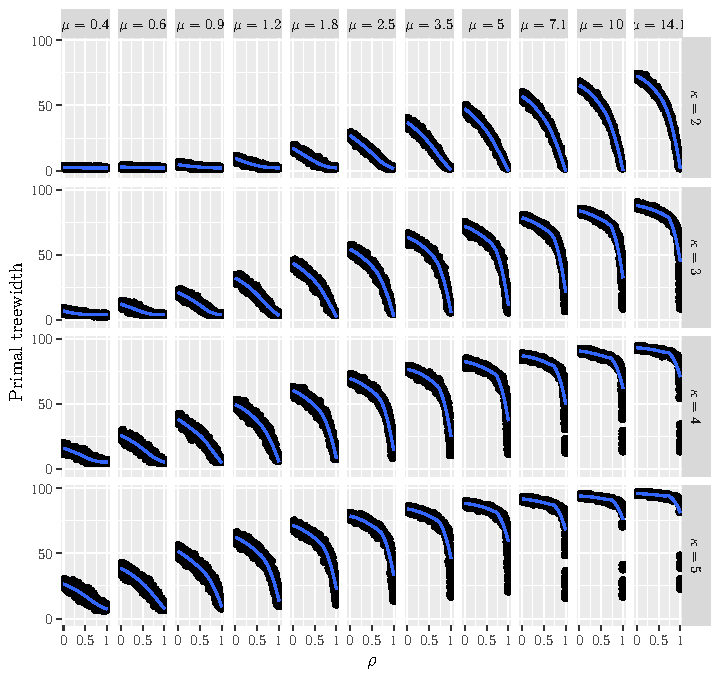
\includegraphics{chapters/comparison/regular_repetitiveness.pdf}
  \caption{The relationship between $\rho$ and primal treewidth for various
    values of $\mu$ and $\kappa$ for $k$-CNF formulas from
    \cref{exp:regular_satisfiability}. Black points represent individual
    instances, and blue lines are smoothed means computed using locally weighted
    smoothing. The values of $\mu$ are rounded to one decimal
    place.}\label{fig:regular_repetitiveness}
\end{figure}

\Cref{fig:regular_repetitiveness} shows the relationship between $\rho$ and
primal treewidth. Except for when both $\mu$ and $\kappa$ are set to very low
values (i.e., the formulas are small in both clause width and the number of
clauses), primal treewidth decreases as $\rho$ increases. This downward trend
becomes sharper as $\mu$ increases, however, not uniformly: it splits into a
roughly linear segment that approaches a horizontal line (for most values of
$\rho$) and a sharply-decreasing segment that approaches a vertical line (when
$\rho$ is close to one). Higher values of $\kappa$ seem to expedite this
transition, i.e., with a higher value of $\kappa$, a lower value of $\mu$ is
sufficient for a smooth downward curve between $\rho$ and primal treewidth to
turn into a combination of a horizontal and a vertical line. While this
behaviour may be troublesome when generating formulas with higher values of
$\mu$ (almost all of which would be unsatisfiable), the relationship between
$\rho$ and primal treewidth is excellent for generating 3-CNF formulas close to
and below the satisfiability threshold of
4.25 \citep{DBLP:journals/ai/CrawfordA96}.

Regarding satisfiability, the proportion of satisfiable 3-CNF formulas drops
from \SI{63.6}{\percent} when $\rho = 0$ to \SI{50.9}{\percent} when $\rho = 1$,
so---while $\rho$ does affect satisfiability---the effect is not significant
enough to influence our experimental setup in the next section.

% It is well-known that there is a sharp transition from satisfiable to
% unsatisfiable 3-CNF formulas at $\mu = 4.25$ regardless of the value of $\nu$
% (this is known as the \emph{satisfiability
% threshold})~\cite{DBLP:journals/ai/CrawfordA96}.

\section{Experimental Results}\label{sec:experiments}

\begin{figure}[t]
  \centering
  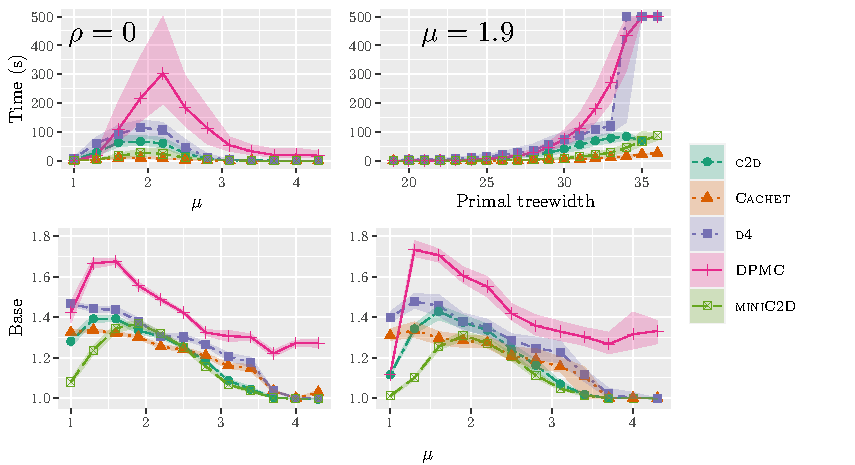
\includegraphics{chapters/comparison/treewidth}
  \caption[Visualisations of the data from \cref{exp:density}. The top-left plot
  shows how the running time of each algorithm changes w.r.t.\ density when
  $\rho = 0$. The top-right plot shows changes in the running time of each
  algorithm w.r.t.\ primal treewidth with $\mu$ fixed at $1.9$. The plots at the
  bottom show how the estimated base of the exponential relationship between
  primal treewidth and the runtime of each algorithm depends on $\mu$. The
  bottom-left plot is for the simple linear model (with shaded regions showing
  standard error), and the bottom-right plot uses the estimates provided by ESA
  (with shaded regions showing \SI{95}{\percent} confidence intervals).]%
  {Visualisations of the data from \cref{exp:density}. The top-left plot shows
    how the running time of each algorithm changes w.r.t.\ density when
    $\rho = 0$. The top-right plot shows changes in the running time of each
    algorithm w.r.t.\ primal treewidth with $\mu$ fixed at $1.9$. The plots at
    the bottom show how the estimated base of the exponential relationship
    between primal treewidth and the runtime of each algorithm depends on $\mu$.
    The bottom-left plot is for the simple linear model (with shaded regions
    showing standard error), and the bottom-right plot uses the estimates
    provided by ESA \protect{\citep{DBLP:conf/gecco/PushakH20}} (with shaded
    regions showing \SI{95}{\percent} confidence intervals).}\label{fig:treewidth}
\end{figure}

% the experimental setup
In this section, we describe three experiments that examine how the running
times of \textsf{WMC} algorithms change w.r.t.\ parameters of our random model.
All experiments were run on Intel Xeon~E5--2630 with Scientific Linux~7,
GCC~10.2.0, Python~3.8.1, R~4.1.0,
\textsc{c2d}~2.20 \citep{DBLP:conf/ecai/Darwiche04},
\textsc{Cachet}~1.22 \citep{DBLP:conf/sat/SangBBKP04},
\textsc{htd}~1.2.0 \citep{DBLP:conf/cpaior/AbseherMW17}, and with no additional preprocessing. With both \textsc{c2d} and \textsc{d4}, we use \textsc{query-dnnf}\footnote{\url{http://www.cril.univ-artois.fr/kc/d-DNNF-reasoner.html}} to compute the numerical answer from the compiled circuit. We omit \textsc{ADDMC} \citep{DBLP:conf/aaai/DudekPV20} from our experiments as it exceeds time and memory limits on too many instances; however, observations about the behaviour of \textsc{DPMC} \citep{DBLP:conf/cp/DudekPV20} apply to \textsc{ADDMC} as well, with the addendum that the tree decomposition implicitly used by \textsc{ADDMC} may have a significantly higher width. \textsc{DPMC} is run with tree decomposition-based planning (using one iteration of \textsc{htd}) and ADD-based execution---the combination that was originally found to be most effective. We restrict our attention to 3-CNF formulas, generate 100 satisfiable instances for each \emph{combination} of parameters, and run each of the five algorithms with a \SI{500}{\second} time limit and an \SI{8}{\gibi\byte} memory limit. While both limits are somewhat low, we prioritise large numbers of instances to increase the accuracy and reliability of our results. Unless stated otherwise, in each plot of this section, lines denote median values, and shaded regions show interquartile ranges. We run the following three experiments, setting $\nu = 70$ in all of them as we found that this produces instances of suitable difficulty.

\begin{experiment}[Density and Primal Treewidth]\label{exp:density}
  Let $\nu = 70$, $\mu$ go from 1 to 4.3 in steps of 0.3, $\rho$ go from 0 to
  0.5 in steps of 0.01, and $\delta = \epsilon = 0$.
\end{experiment}

\begin{experiment}[$\delta$]\label{exp:delta}
  Let $\nu = 70$, $\mu = 2.2$\footnote{\Cref{exp:density} shows this density to
    be the most challenging for \textsc{DPMC}.},
  $\rho = 0$, $\delta$ go from 0 to 1 in steps of 0.01, and $\epsilon = 0$.
\end{experiment}

\begin{experiment}[$\epsilon$]\label{exp:epsilon}
  Same as \cref{exp:delta} but with $\delta = 0$ and $\epsilon$ going from 0 to
  1 in steps of 0.01.
\end{experiment}

% c2d and d4 are the most memory-hungry
In each experiment, the proportion of algorithm runs that timed out never
exceeded \SI{3.8}{\percent}. While in \cref{exp:density} only \SI{1}{\percent}
of experimental runs ran out of memory, the same percentage was higher in
\cref{exp:delta,exp:epsilon}---10 and \SI{12}{\percent}, respectively.
\textsc{d4} \citep{DBLP:conf/ijcai/LagniezM17} and
\textsc{c2d} are the algorithms that
experienced the most issues fitting within the memory limit, accounting for
\SIrange{66}{72}{\percent} and \SIrange{28}{33}{\percent} of such instances,
respectively. We exclude the runs that terminated early due to running out of
memory from the rest of our analysis.

% Peaks w.r.t. density: DPMC different from other WMC algorithms which are
% different from #SAT algorithms
In \cref{exp:density}, we investigate how the running time of each algorithm
depends on the density and primal treewidth by varying both $\mu$ and $\rho$.
The results are in \cref{fig:treewidth}. The first thing to note is that the
peak hardness w.r.t.\ density occurs at around 1.9 for all algorithms except for
\textsc{DPMC}, which peaks at 2.2 instead.\footnote{While exact values might be hard to read from the plot, they are confirmed by numerical data.} This finding is consistent with previous work, which shows \textsc{Cachet} to peak at 1.8 \citep{DBLP:conf/sat/SangBBKP04}.\footnote{For comparison, $\#\SAT{}$ algorithms have been observed to peak at densities 1.2 and 1.5 \citep{DBLP:conf/aaai/Pehoushek00}.}

\begin{figure}[t]
  \centering
  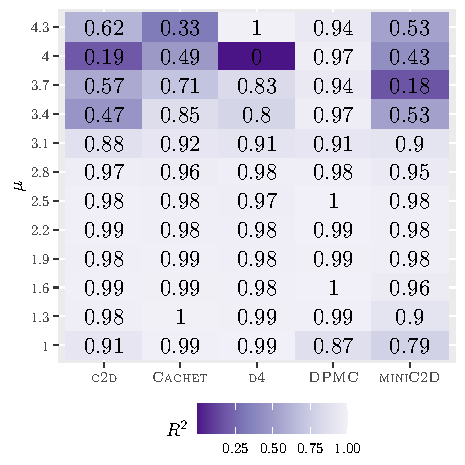
\includegraphics{chapters/comparison/r2}
  \caption{The coefficients of determination (rounded to one decimal place) of
    all the linear models fitted for the top-right subplot of
    \cref{fig:treewidth}.}\label{fig:r2}
\end{figure}

\begin{figure}[t]
  \centering
  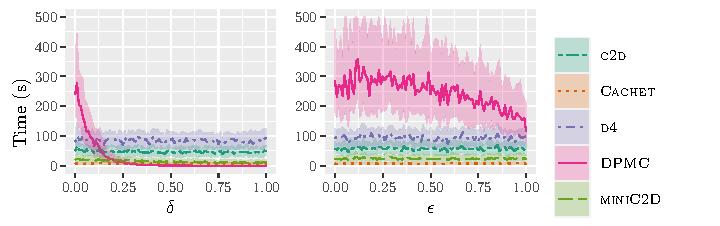
\includegraphics{chapters/comparison/delta_epsilon}
  \caption{Changes in the running time of each algorithm as a result of changing
    $\delta$ (on the left-hand side) and $\epsilon$ (on the right-hand side)
    according to the data from
    \cref{exp:delta,exp:epsilon}.}\label{fig:delta_epsilon}
\end{figure}

The other question we want to investigate using this experiment is how each algorithm scales w.r.t.\ primal treewidth. The top-right plot in \cref{fig:treewidth} shows this relationship for a fixed value of $\mu$, and one can see some evidence that the running time of \textsc{DPMC} grows faster w.r.t.\ primal treewidth than the running time of the other algorithms. We use two statistical techniques to quantify this growth: a simple linear regression model and the empirical scaling analyzer (ESA)~v2\footnote{\url{https://github.com/YashaPushak/ESA}} \citep{DBLP:conf/gecco/PushakH20}. In both cases, for each algorithm and value of $\mu$ in \cref{exp:density}, we select the median runtime for all available values of primal treewidth. In the former case, we fit the model $\ln t \sim \alpha w + \beta$, where $t$ is the median running time of the algorithm, $w$ is the primal treewidth, and $\alpha$ and $\beta$ are parameters.\footnote{Similar statistical analyses have been used to investigate polynomial-to-exponential phase transitions in \SAT{} \citep{DBLP:journals/constraints/CoarfaDASV03} and the behaviour of \SAT{} solvers on CNF-XOR formulas \citep{DBLP:conf/ijcai/DudekMV17}.} In other words, this model attempts to express median running time as $e^\beta{(e^\alpha)}^w$. In the latter case, we run ESA with 1001 bootstrap samples, a window of 101, and use the first \SI{30}{\percent} of the data for training.

% DPMC scales worse w.r.t. primal treewidth (across all densities)
The results of both models are qualitatively the same (with the exception of \textsc{DPMC} run on instances with $\mu = 1$) and are displayed at the bottom of \cref{fig:treewidth}. We find that, indeed, \textsc{DPMC} scales worse w.r.t.\ primal treewidth than any other algorithm across all values of $\mu$ and is the only algorithm that does not become indifferent to primal treewidth when faced with high-density formulas. A second look at the top-left subplot of \cref{fig:treewidth} suggests an explanation for the latter observation. The running times of all algorithms except for \textsc{DPMC} approach zero when $\mu > 3$ while the median running time of \textsc{DPMC} approaches a small non-zero constant instead. This observation also explains why \cref{fig:r2} shows that the fitted models fail to explain the data for non-ADD algorithms running on high-density instances---the running times are too small to be meaningful. In all other cases, an exponential relationship between primal treewidth and runtime fits the experimental data remarkably well.

% miniC2D is good at low-density high-primal-treewidth instances
Another thing to note is that \textsc{miniC2D} \citep{DBLP:conf/ijcai/OztokD15} is the only algorithm that exhibits a clear low-high-low pattern in the bottom subplots of \cref{fig:treewidth}. To a smaller extent, the same may apply to \textsc{c2d} and \textsc{DPMC} as well, although the evidence for this is limited due to relatively large gaps between different values of $\mu$ in \cref{exp:density}. In contrast, the running times of \textsc{Cachet} and \textsc{d4} remain dependent on primal treewidth even when the density of the \textsf{WMC} instance is very low, suggesting that \textsc{miniC2D} should have an advantage on low-density high-primal-treewidth instances.

% A median instance with all weights equal to 0.5 is about three times easier
% than a median instance with completely random weights.
Finally, \cref{exp:delta,exp:epsilon} investigate how changing the numerical values of weights can simplify a \textsf{WMC} instance. The results are in plotted \cref{fig:delta_epsilon}. As expected, the running time of all algorithms other than \textsc{DPMC} stay the same regardless of the value of $\delta$ or $\epsilon$. The running time of \textsc{DPMC}, however, experiences a sharp (exponential?) decline with increasing $\delta$. The decline w.r.t. $\epsilon$ is also present, although significantly less pronounced and with high variance.

How are these random instances different from real data? As a representative sample, we take the \textsf{WMC} encodings of Bayesian networks created using the method by \citet{DBLP:conf/aaai/SangBK05} as found in the experimental setup\footnote{\url{https://github.com/vardigroup/DPMC/releases}} of the \textsc{DPMC} paper \citep{DBLP:conf/cp/DudekPV20}. A typical \textsf{WMC} instance has $\nu = 200$ variables, half of which have equal weights (i.e., $\epsilon = 0.5$), an average clause width of $\kappa = 2.6$, a density of $\mu = 2.5$, and a primal treewidth of 28. Our random instances have fewer variables and (for the most part) lower density. Another important difference is that our instances are in $k$-CNF whereas a typical encoding of a Bayesian network has many two-literal clauses mixed with clauses of various longer widths. Despite real instances having more variables, their primal treewidth is rather low. Perhaps this partially explains why the performance of \textsc{DPMC} is in line with the performance of all other algorithms on traditionally-used benchmarks \citep{DBLP:conf/cp/DudekPV20} despite struggling with most of our random data.

To sum, we found that \textsc{c2d} and
\textsc{d4} are the most memory-intensive
algorithms, \textsc{Cachet} is great on random
instances in general, \textsc{miniC2D} exceeds
on low-density high-primal-treewidth instances, and
\textsc{DPMC} is at its best on low-density
low-primal-treewidth instances. Furthermore, a median instance with all weights
equal to each other is about three times easier for \textsc{DPMC} than a median
instance with random weights. Another important observation is about how peak
hardness w.r.t. density depends on the algorithm: \textsc{DPMC} peaks at a
higher density than all other \textsc{WMC} algorithms, which peak at a higher
density than (some) $\#\SAT{}$ algorithms.

\section{Conclusions and Future Work}

In this paper, we studied the behaviour of and differences among \textsf{WMC}
algorithms on random instances generated by a standard model for $k$-CNF
formulas extended with parameters that control primal treewidth and literal
weights. Among other things, we established statistical evidence for the
existence of an exponential relationship between primal treewidth and the
running time of all \textsf{WMC} algorithms. The running time of ADD-based
algorithms was observed to peak at a higher density, scale worse w.r.t. primal
treewidth, and depend negatively on repeating weight values compared to
algorithms based on search or knowledge compilation. These observations can, to
some degree, be extended to a closely related weighted projected model counting
algorithm \citep{DBLP:conf/sat/DudekPV21} as well as to other applications of
ADDs more generally, e.g., probabilistic
inference \citep{DBLP:conf/ijcai/ChaviraD07,DBLP:conf/uai/GogateD11} and
stochastic planning \citep{DBLP:conf/uai/HoeySHB99}.

One limitation of our work is that variability in primal treewidth was achieved
via a parameter, and this could bias randomness in some unexpected way (although
it is encouraging that there is only a slight decrease in the proportion of
satisfiable instances between $\rho=0$ and $\rho = 1$). Perhaps a theoretical
investigation of the proposed model is warranted, including a characterisation
of how $\rho$ influences primal treewidth and the structure of the primal graph
more generally. Since treewidth is widely used in parameterised complexity
\citep{DBLP:series/txcs/DowneyF13}, formally establishing a connection with
$\rho$ could make our random model useful for a variety of other hard
computational problems.

To keep the number of experiments feasible, we restricted our attention to 3-CNF
formulas, although, of course, this is not very representative of real-world
\textsf{WMC} instances. The model could be adapted to generate non-$k$-CNF
formulas, and perhaps a more representative structure could be achieved by
introducing new variables that clauses define to be equivalent to select
conjunctions of literals as is done in one of the \textsf{WMC} encodings for
Bayesian networks \citep{DBLP:conf/kr/Darwiche02}.

% It would also be interesting to see whether \textsf{WMC}
% algorithms differ in their ability to effectively handle a `shattered' solution
% space, where most solutions are distant to each other w.r.t. the Hamming
% distance \cite{DBLP:journals/rsa/AchlioptasCR11,DBLP:conf/ijcai/DudekMV17}.

\chapter{Generating Random WMC Instances} \label{chapter:comparison}

\section{Introduction}

% WMC
Weighted model counting (\textsf{WMC})---a weighted generalisation of
propositional model counting
($\#\SAT{}$) \citep{DBLP:journals/ai/ChaviraD08}---has emerged as a powerful
computational framework for problems in a variety of domains. In particular,
\textsf{WMC} has been used to perform probabilistic inference for graphical
models such as Bayesian networks and Markov random
fields \citep{DBLP:conf/ecai/BartKLM16,DBLP:conf/ijcai/ChaviraD05,DBLP:conf/sat/ChaviraD06,DBLP:conf/kr/Darwiche02,DBLP:conf/aaai/SangBK05},
probabilistic programs \citep{DBLP:journals/pacmpl/HoltzenBM20}, and
probabilistic logic programs \citep{DBLP:journals/tplp/FierensBRSGTJR15}. More
recently, \textsf{WMC} was used in the context of neural-symbolic artificial
intelligence as well \citep{DBLP:conf/icml/XuZFLB18}. Extensions of \textsf{WMC}
add support for continuous variables \citep{DBLP:conf/ijcai/BellePB15}, infinite
domains \citep{DBLP:conf/aaai/Belle17}, and first-order
logic \citep{DBLP:conf/ijcai/BroeckTMDR11,DBLP:journals/cacm/GogateD16} and
generalise the definition to support arbitrary pseudo-Boolean functions instead
of clauses \citep{DBLP:conf/sat/DilkasB21}.
Exact \textsf{WMC} algorithms can be broadly classified as based on
search \citep{DBLP:conf/sat/SangBBKP04,DBLP:conf/ijcai/SharmaRSM19}, knowledge
compilation \citep{DBLP:conf/ecai/Darwiche04,DBLP:conf/ijcai/LagniezM17,DBLP:conf/ijcai/OztokD15}, and
dynamic programming \citep{DBLP:conf/aaai/DudekPV20,DBLP:conf/cp/DudekPV20}. Other alternatives include approximate \citep{DBLP:conf/aaai/RenkensKBR14} and parallel algorithms \citep{DBLP:conf/pgm/DalLL18,DBLP:conf/esa/FichteHWZ18}, hybrid approaches \citep{DBLP:conf/sat/HecherTW20}, quantum computing \citep{DBLP:conf/ecai/Riguzzi20}, and reduction to model counting \citep{DBLP:conf/ijcai/ChakrabortyFMV15}.

% motivation for the problem
Recent papers that include experimental comparisons of \textsf{WMC}
algorithms show many of them performing very similarly
overall \citep{DBLP:conf/aaai/DudekPV20,DBLP:conf/cp/DudekPV20} but with
overwhelming differences when run on specific subsets of
data \citep{DBLP:conf/uai/DilkasB21,DBLP:conf/sat/DilkasB21,DBLP:conf/ijcai/LagniezM17}.
Examples of such segregating data sets include bipartite Bayesian networks by
\citet{DBLP:conf/aaai/SangBK05} and
relational Bayesian networks by
\citet{DBLP:journals/ijar/ChaviraDJ06}
that encode reachability in graphs under node deletion. So far, such performance
differences remain unexplained. However, knowledge about the nature of these
differences can inform our choices and aid in further algorithmic developments.
Moreover, identifying performance predictors of algorithms is often an important
step in developing a portfolio approach to the
problem \citep{DBLP:journals/jair/XuHHL08}. Lastly, if new algorithms are always
tested on the same set of benchmarks, eventually they may become somewhat fitted
to the particular characteristics of those instances, leading to algorithms that
may perform worse when run on new types of
data \citep{DBLP:conf/cec/HossainALA10}.

% related work on SAT
Both theoretical and experimental analysis of \SAT{} (and, to a lesser extent,
$\#\SAT{}$) algorithms on random instances is a rich area of research spanning
almost forty years. Variations of some of the first random models ever
proposed \citep{DBLP:journals/dam/FrancoP83,DBLP:journals/siamcomp/PurdomB83}
continue to be instrumental up to this day for, e.g., establishing the location
of the threshold between satisfiable and unsatisfiable
instances \citep{DBLP:conf/focs/AchlioptasM02} and efficiently approximating
$\#\SAT{}$ \citep{DBLP:conf/icalp/GalanisG0Y20}. Other random models consider
non-uniform variable frequencies \citep{DBLP:conf/ijcai/AnsoteguiBL09}, fixing
the number of times each variable occurs both positively and
negatively \citep{DBLP:journals/cpc/Coja-OghlanW18}, and adding other constraints
such as cardinality and `exclusive or' \citep{DBLP:conf/ijcai/PoteJM19}. In
contrast, only one \textsf{WMC} algorithm so far has been analysed using random
instances \citep{DBLP:conf/sat/SangBBKP04,DBLP:conf/sat/SangBK05}. Similarly,
while there is a recent attempt \citep{DBLP:conf/cp/DilkasB20} to compare
\textsf{WMC} algorithms on random instances of a particular application of
\textsf{WMC} (i.e., probabilistic logic programs), it fails to discern any
meaningful differences among the algorithms. The goal of this paper is to
explain some of the differences between \textsf{WMC} algorithms via an
experimental study that uses random instances.

% parameters for SAT
Experimental work investigating how \SAT{} algorithms behave on random
instances is typically centred around parameters that describe each instance
independently of its size. The most well-known parameter is the ratio of clauses
to variables (i.e., \emph{(clause) density}). Early work in the area
showed random 3-\SAT{} instances to be at their hardest when density is
around 4.25 \citep{DBLP:conf/aaai/MitchellSL92}. Later work revealed that the
interaction between density and empirical hardness is much more
solver-dependent \citep{DBLP:journals/constraints/CoarfaDASV03}. Many other
parameters such as heterogeneity, locality, and modularity have emerged from
attempts to generate random instances similar to industry benchmarks for
\SAT{} \citep{DBLP:conf/ijcai/AnsoteguiBL09,DBLP:conf/tacas/BlasiusFS19,DBLP:journals/ai/Giraldez-CruL16,DBLP:conf/ijcai/Giraldez-CruL17}.

% parameters for WMC
What parameter(s) are most appropriate to study \textsf{WMC}? Theoretical upper
bounds on the performance of various \textsf{WMC} algorithms typically include a
factor exponential in the primal treewidth of the input formula (or a closely
related
notion) \citep{DBLP:journals/jair/BacchusDP09,DBLP:journals/jacm/Darwiche01,DBLP:conf/ecai/Darwiche04,DBLP:conf/sat/SangBBKP04}.
However---as we show in \cref{sec:model}---instances generated by a standard
random model for $k$-CNF formulas fail to exhibit enough variance in primal
treewidth for us to infer its effect on the behaviour of the algorithms.
Therefore, we present an extension of this model with a parameter that
influences primal treewidth. The performance of \textsf{WMC} algorithms that use
data structures called \emph{algebraic decision diagrams}
(ADDs) \citep{DBLP:journals/fmsd/BaharFGHMPS97} is also known to depend on the
numerical values of
weights \citep{DBLP:conf/aaai/DudekPV20,DBLP:conf/cp/DudekPV20}. Thus, our random
model also includes two parameters that control redundancies in these values.
We also
investigate the effect of redundant weight values (e.g., having weights set to
zero and one or having the same weight repeat many times) on the running times
of the algorithms.

In addition to introducing a new random model for \textsf{WMC} instances, the
contributions of this paper include several key experimental findings about the
behaviour of \textsf{WMC} algorithms---namely,
\textsc{c2d}\footnote{\url{http://reasoning.cs.ucla.edu/c2d/}} \citep{DBLP:conf/ecai/Darwiche04},
\textsc{Cachet}\footnote{\url{https://cs.rochester.edu/u/kautz/Cachet/}} \citep{DBLP:conf/sat/SangBBKP04},
\textsc{d4}\footnote{\url{https://www.cril.univ-artois.fr/KC/d4.html}} \citep{DBLP:conf/ijcai/LagniezM17},
\textsc{DPMC}\footnote{\url{https://github.com/vardigroup/dpmc}} \citep{DBLP:conf/cp/DudekPV20},
and
\textsc{miniC2D}\footnote{\url{http://reasoning.cs.ucla.edu/minic2d/}} \citep{DBLP:conf/ijcai/OztokD15}---on
random instances. First, we show that the easy-hard-easy pattern with respect to
(w.r.t.) density is different for dynamic programming algorithms than it is for
all other algorithms. Second, we present statistical evidence that all the
algorithms scale exponentially w.r.t.\ primal treewidth and estimate how the
base of that exponential changes w.r.t.\ density. Third, we show how the
performance of ADD-based algorithms gradually improves w.r.t the proportion of
weights that have repeating values and sharply improves w.r.t.\ the proportion
of weights set to zero and one.

% 1. Other parameters include structural entropy
% \cite{DBLP:journals/access/LinWN21}, the proportion of clauses that have at
% most one negative literal has also been suggested as a parameter of
% interest~\cite{DBLP:journals/amai/MaarenN05}.
% 2. Maybe somewhere: relationship between primal treewidth and modularity
% 3. Just like one might choose a different propositional satisfiability
% (\SAT{}) solver based on information about the problem instance at hand (e.g.,
% `is the instance known to be satisfiable?', `was it randomly generated?', `is
% it an industrial instance?')~\cite{DBLP:journals/jair/XuHHL08},
% 4. It was also observed that replacing real numbers with addition and
% multiplication with an arbitrary commutative semiring allows \textsf{WMC} to
% subsume a variety of other problems such as most probable explanation,
% shortest path, and gradient
% computations~\cite{DBLP:journals/ijar/BelleR20,DBLP:journals/japll/KimmigBR17}.
% 5. Having these parameters in the model allows us to look not just at the
% effects of density or primal treewidth on the running times of \textsf{WMC}
% algorithms but also at the interaction between these two parameters of
% interest.

\section{Preliminaries}

% \footnote{Also known by many other names such as Gaifman, (variable)
% interaction, and variable incidence graph.}

By \emph{variable}, we always mean a Boolean variable. A \emph{literal} is
either a variable (say, $v$) or its negation (denoted $\neg v$), respectively
called \emph{positive} and \emph{negative} literal. A \emph{clause} is a
disjunction of literals. A \emph{formula} is any well-formed expression
consisting of variables, negation, conjunction, and disjunction. A formula is in
\emph{conjunctive normal form} (CNF) if it is a conjunction of clauses, and it
is in $k$-CNF if every clause has exactly $k$ literals. While we use the
set-theoretic notation for CNF formulas (e.g., writing $c \in \phi$ to mean that
clause $c$ is one of the clauses in formula $\phi$), duplicate clauses are still
allowed. The \emph{primal graph} of a CNF formula is a graph that has a node for
every variable, and there is an edge between two variables if they coappear in
some clause. The \emph{treewidth} of a graph $G$ measures how similar $G$
is to a tree and is defined as the smallest \emph{width} of any \emph{tree
  decomposition} of $G$ \citep{DBLP:journals/jct/RobertsonS84}. The \emph{primal
  treewidth} of a formula is the treewidth of its primal graph.

Given a CNF formula $\phi$, \SAT{} is a decision problem that asks whether there
exists a way to assign values to all variables in $\phi$ such that $\phi$
evaluates to true. Such a formula is said to be \emph{satisfiable}; otherwise,
it is \emph{unsatisfiable}. $\#\SAT{}$ is a problem that asks to count the
number of such assignments. \textsf{WMC} extends $\#\SAT{}$ with a weight
function on literals and asks to compute the sum of the weights of the models of
the given formula, where the weight of a model is the product of the weights of
the literals in it \citep{DBLP:journals/ai/ChaviraD08}. For example, the
\textsf{WMC} of the formula $x \lor y$ with a weight function $w\colon \{\,x, y,
\neg x, \neg y\,\} \to \mathbb{R}_{\ge 0}$ defined as $w(x) = 0.3$, $w(y) = 0.2$,
$w(\neg x) = 0.7$, $w(\neg y) = 0.8$ is $w(x)w(y)+w(x)w(\neg y)+w(\neg x)w(y) =
0.3 \times 0.2 + 0.3 \times 0.8 + 0.7 \times 0.2 = 0.44$.

\section{Background on \textsf{\textmd{WMC}} Algorithms}\label{sec:background}

In this section, we briefly review the three major approaches to \textsf{WMC}---search, knowledge compilation, and dynamic programming---and their corresponding algorithms. The main search-based \textsf{WMC} algorithm \textsc{Cachet} \citep{DBLP:conf/sat/SangBBKP04} is based on a conflict-driven clause learning \SAT{} solver \citep{DBLP:conf/dac/MoskewiczMZZM01}, which is then extended with a component caching scheme and adapted to counting.

\emph{Knowledge compilation} refers to transformations of propositional formulas
into more restrictive formats that make various operations (such as model
counting) tractable in the size of the representation
\citep{DBLP:journals/jair/DarwicheM02}.
\textsc{c2d} \citep{DBLP:conf/ecai/Darwiche04},
\textsc{d4} \citep{DBLP:conf/ijcai/LagniezM17}, and
\textsc{miniC2D} \citep{DBLP:conf/ijcai/OztokD15}
are all algorithms of this type. \textsc{c2d} compiles to deterministic
decomposable negation normal form
(d-DNNF) \citep{DBLP:journals/jancl/Darwiche01}. Similarly, \textsc{d4} compiles
to decision-DNNF (also known as decomposable decision
graphs) \citep{DBLP:conf/aaai/FargierM06}. The only difference between d-DNNF and
decision-DNNF is that decision-DNNF has if-then-else constructions instead of
disjunctions \citep{DBLP:conf/ijcai/LagniezM17}. Finally,
\textsc{miniC2D} compiles to decision-SDDs---a
subset of sentential decision diagrams (SDDs) that form a subset of
d-DNNF \citep{DBLP:conf/ijcai/Darwiche11}.

All of the algorithms mentioned above execute in exactly the same way regardless of whether computing \textsf{WMC} or $\#\SAT{}$. Two recent \textsf{WMC} algorithms instead use data structures whose size (and thus the runtime of the algorithm) depends on the numerical values of weights. These data structures are representations of \emph{pseudo-Boolean functions}, i.e., functions of the form $f\colon 2^X \to \mathbb{R}_{\ge 0}$, where $X$ is a set, and $2^X$ denotes its powerset. \textsc{ADDMC} is the first such algorithm \citep{DBLP:conf/aaai/DudekPV20}. It uses ADDs to represent pseudo-Boolean functions, combining and simplifying them in a bottom-up dynamic programming fashion. Since the size of an ADD for $f$ depends on the cardinality of the range of $f$ \citep{DBLP:journals/fmsd/BaharFGHMPS97}, the performance of the algorithm is sensitive to the numerical values of weights, e.g., to how frequently they repeat. \textsc{DPMC} extends \textsc{ADDMC} in two ways \citep{DBLP:conf/cp/DudekPV20}. First, \textsc{DPMC} allows for the order and nesting of operations on ADDs to be determined from an approximately-minimal-width tree decomposition rather than by heuristics.\footnote{There is also a recent line of work in using tree decompositions to guide the heuristics of search-based model counters \citep{DBLP:conf/cp/KorhonenJ21}.} Second, tensors are offered as an alternative to ADDs.

In all known parameterised complexities of \textsf{WMC} algorithms, the
exponential factor is a function of primal treewidth or a closely related
parameter. Interestingly, \textsc{c2d} is specifically designed to handle high
primal treewidth (which the author refers to as
\emph{connectivity} \citep{DBLP:conf/ijcai/Darwiche99}) and improves upon an
earlier algorithm that has $\mathcal{O}(mw2^w)$ time complexity, where $m$ is
the number of clauses, and $w$ is the width of the decomposition tree which is
known to be at most primal
treewidth \citep{DBLP:journals/jacm/Darwiche01,DBLP:conf/ecai/Darwiche04}. While
the complexity of \textsc{Cachet} was not analysed directly, the algorithm is
based on component caching which is known to have a
$2^{\mathcal{O}(w)}n^{\mathcal{O}(1)}$ time complexity, where $n$ is the number
of variables, and $w$ is the branchwidth of the underlying
hypergraph \citep{DBLP:journals/jair/BacchusDP09,DBLP:conf/sat/SangBBKP04}, which
is known to be within a constant factor of primal
treewidth \citep{DBLP:journals/jct/RobertsonS91}. Similarly, the complexity of
\textsf{DPMC} is not described in the paper, although the authors define a
notion of width $w$ that is at most primal treewidth plus one and estimate the
running time of the (execution part of the) algorithm to be proportional to
$2^w$ \citep{DBLP:conf/cp/DudekPV20}.

\section{Random $k$-CNF Formulas with Varying Primal
  Treewidth}\label{sec:model}

\paragraph{Notation.}
For any graph $G$, we write $\mathcal{V}(G)$ for its set of nodes and
$\mathcal{E}(G)$ for its set of edges. Let $S$ be a finite set. We write
$\mathcal{U}S$ for the discrete uniform probability distribution on $S$. We
represent any other probability distribution as a pair $(S, p)$ where $p\colon S
\to [0, 1]$ is a probability mass function. For any probability distribution
$\mathcal{P}$, we write $x \leftlsquigarrow \mathcal{P}$ to denote the act of
sampling $x$ from $\mathcal{P}$. For instance, $x \leftlsquigarrow (\{\, 1, 2 \,\}, \{\, 1 \mapsto 0.1, 2 \mapsto 0.9 \,\})$ means that $x$ becomes equal to $1$ with probability $0.1$ or to $2$ with probability $0.9$.

Our random model is based on the following parameters:
\begin{itemize}
\item the number of variables $\nu \in \mathbb{N}^+$,
\item density $\mu \in \mathbb{R}_{>0}$,
\item clause width $\kappa \in \mathbb{N}^+$ (for $k$-CNF formulas, $\kappa =
  k$),
\item a parameter $\rho \in [0, 1]$ that influences the primal treewidth of
  the formula,
\item the proportion $\delta \in [0, 1]$ of variables $x$ such that $w(x) = 1$
  and $w(\neg x) = 0$ or $w(x) = 0$ and $w(\neg x) = 1$,
\item and the proportion $\epsilon \in [0, 1-\delta]$ of variables $x$ such that
  $w(x) = w(\neg x) = 0.5$.
\end{itemize}
The first three parameters are the standard parameters used to generate random
$k$-CNF formulas with $\nu\mu$ clauses (up to rounding). We expect to observe
(possibly different) values of $\mu$ that maximize the running time of each
algorithm for fixed values of $\nu$ and $\kappa$. Parameters $\delta$ and
$\epsilon$ control the numerical values of weights and are part of the model
because the running time of \textsc{DPMC} \citep{DBLP:conf/cp/DudekPV20}---and
other algorithms based on ADDs---depends on these values. Weights such as zero
and one are particularly `simplifying' because they are respectively the
additive and multiplicative identities. Having them propagate through the
algorithm reduces the size of many ADDs used by \textsc{DPMC}, making the
algorithm more efficient. Including many copies of the same weight (e.g., 0.5)
can similarly simplify ADDs as well. Other \textsf{WMC} algorithms are
indifferent to the numerical values of weights.

\begin{algorithm}[t]
  \caption{Generating a random formula.}\label{alg:random}
  \SetKwData{kcnf}{kcnf}
  \SetKwFunction{NewVariable}{NewVariable}
  \SetKwProg{Fn}{Function}{:}{}
  \KwIn{$\nu,\kappa \in \mathbb{N}^+$ such that $\kappa < \nu$, $\mu \in
    \mathbb{R}_{>0}$, $\rho \in [0, 1]$.}
  \KwOut{A $k$-CNF formula $\phi$.}
  $\phi \gets \text{empty CNF formula}$\;
  $G \gets \text{empty graph}$\;
  \For{$i \gets 1$ \KwTo $\lfloor \nu\mu \rfloor$}{
    $X \gets \emptyset$\;
    \For{$j \gets 1$ \KwTo $\kappa$}{
      $x \gets \NewVariable{$X$, $G$}$\;
      $\mathcal{V}(G) \gets \mathcal{V}(G) \cup \{\, x \,\}$\;\label{line:7}
      $\mathcal{E}(G) \gets \mathcal{E}(G) \cup \{\, \{\,x, y\,\} \mid y \in X
      \,\}$\;\label{line:8}
      $X \gets X \cup \{\, x \,\}$\;\label{line:9}
    }
    $\phi \gets \phi \cup \{\, l \leftlsquigarrow \mathcal{U}\{\, x, \neg x \,\}
    \mid x \in X \,\}$\;\label{line:construct_clause}
  }
  \Return{$\phi$}\;
  \Fn{\NewVariable{$X$, $G$}}{
    $N \gets \{\, e \in \mathcal{E}(G) \mid |e \cap X| = 1
    \,\}$\;\label{line:13}
    \If{$N = \emptyset$}{
      \Return{$x \leftlsquigarrow \mathcal{U}(\{\, x_1, x_2, \dots, x_\nu \,\}
        \setminus X)$}\;
    }
    \nosemic\Return{$x \leftlsquigarrow \left(\{\, x_1, x_2, \dots, x_\nu \,\}
        \setminus X,\vphantom{\frac{|\{\, z \in X \mid \{\,y, z\,\} \in
            \mathcal{E}(G) \,\}|}{|N|}}\right.$}\;
      \pushline\dosemic$\left. y \mapsto \frac{1 - \rho}{\nu - |X|} +
        \rho\frac{|\{\, z \in X \mid \{\,y, z\,\} \in \mathcal{E}(G)
          \,\}|}{|N|}\right)$\; \label{line:return}
  }
\end{algorithm}

The process behind generating random $k$-CNF formulas is summarized as
\cref{alg:random}. For the rest of this section, let $x_1, x_2, \dots, x_\nu$ be
the variables of the formula under construction. We simultaneously construct
both formula $\phi$ and its primal graph $G$.\footnote{The idea to directly take
  the primal graph into consideration while generating the formula is new---cf.
  random \SAT{} instance generators based on, e.g., adversarial evolution
  \citep{DBLP:conf/cec/HossainALA10} and community structure
  \citep{DBLP:journals/ai/Giraldez-CruL16}.} Each iteration of the first for-loop
adds a clause to $\phi$. This is done by constructing a set $X$ of variables to
be included in the clause, and then randomly adding either $x$ or $\neg x$ to
the clause for each $x \in X$ on \cref{line:construct_clause}. Function
\texttt{NewVariable} randomly selects each new variable $x$, and
\cref{line:7,line:8,line:9} add $x$ to the graph and the formula while also
adding edges between $x$ and all the other variables in the clause. To select
each variable, \cref{line:13} defines set $N$ to contain all edges with exactly
one endpoint in $X$. The edges that will be added to $G$ by \cref{line:8} will
form a subset of $N$. If $N = \emptyset$, we select the variable uniformly at
random (u.a.r.) from all viable candidates. Otherwise, $\rho$ determines how
much we bias the uniform distribution towards variables that would introduce the
smallest number of new edges to $G$.

When $\rho=0$, \cref{alg:random} reduces to what has become the standard random
model for $k$-CNF formulas. Equivalently to \citet{DBLP:journals/dam/FrancoP83},
we independently sample a fixed number of clauses, each clause has no duplicate
variables, and each variable becomes either a positive or a negative literal
with equal probabilities. At the other extreme, when $\rho = 1$, the first
variable of a clause is still chosen u.a.r., but all other variables are chosen
from those that already coappear in a clause (if possible). The probability that
a variable is selected to be included in a clause scales linearly w.r.t.\ the
proportion of edges in $N$ that would be repeatedly added to $G$ if the variable
$y$ was added to the clause. This is an arbitrary choice (which appears to work
well, see \cref{sec:remarks}) although alternatives (e.g., exponential scaling)
could be considered. As long as $\rho < 1$, every $k$-CNF formula retains a
positive probability of being generated by the algorithm.

To transform the generated formula into a \textsf{WMC} instance, we need
to define weights on literals.\footnote{Note that algorithms such as
  \textsc{DPMC} and
  \textsc{ADDMC} \citep{DBLP:conf/aaai/DudekPV20,DBLP:conf/cp/DudekPV20} support
  a more flexible way of assigning weights that can lead to significant
  performance improvements \citep{DBLP:conf/uai/DilkasB21,DBLP:conf/sat/DilkasB21}.} We want to partition all variables into three groups: those with weights equal to zero and one, those with weights equal to 0.5, and those with arbitrary weights, where the size of each group is determined by $\delta$ and $\epsilon$. To do this, we sample a permutation $\pi \leftlsquigarrow \mathcal{U}S_\nu$ (where $S_\nu$ is the permutation group on $\{1, 2, \dots, \nu \}$), and assign to each \emph{variable} $x_n$ a weight drawn u.a.r.\ from
\begin{itemize}
\item $\mathcal{U}\{\,0, 1\,\}$ if $\pi(n) \le \nu\delta$,
\item $\mathcal{U}\{\,0.5\,\}$ if $\nu\delta < \pi(n) \le \nu\delta +
  \nu\epsilon$,
\item and $\mathcal{U}\{\, 0.01, 0.02, \dots, 0.99 \,\}$\footnote{For
    convenience, we represent $(0, 1)$ as 99 discrete values.} if $\pi(n) >
  \nu\delta + \nu\epsilon$.
\end{itemize}
We extend these weights to weights on \emph{literals} by choosing the weight of
each positive literal to be equal to the weight of its variable, and the weight
of each negative literal to be such that $w(x) + w(\neg x) = 1$ for all
variables $x$. This restriction is to ensure consistent answers among the
algorithms.

\begin{example}\label{example:algorithm}
  Let $\nu = 5$, $\mu = 0.6$, $\kappa = 3$, $\rho = 0.3$, $\delta = 0.4$,
  and $\epsilon = 0.2$ and consider how \cref{alg:random} generates a random
  instance. Since $\kappa = 3$, and $\lfloor\nu\mu\rfloor = 3$,
  the algorithm will generate a 3-CNF formula with three clauses.

  For the first variable of the first clause, we are choosing u.a.r.\ from $\{\,
  x_1, x_2, \dots, x_5 \,\}$. Suppose the algorithm chooses $x_5$. Graph $G$
  then gets its first node but no edges. The second variable is chosen u.a.r.
  from $\{\, x_1, x_2, x_3, x_4 \,\}$. Suppose the second variable is $x_2$.
  Then $G$ gets another node and its first edge between $x_2$ and $x_5$. The
  third variable in the first clause is similarly chosen u.a.r.\ from $\{\, x_1,
  x_3, x_4 \,\}$ because the only edge in $G$ has both endpoints in $X = \{\,
  x_2, x_5 \,\}$, and so $N = \emptyset$. Suppose the third variable is $x_1$.
  Graph $G$ becomes a triangle connecting $x_1$, $x_2$, and $x_5$. Each of
  the three variables is then added to the clause as either a positive or a
  negative literal (with equal probabilities). Thus, the first clause becomes,
  e.g., $\neg x_5 \lor x_2 \lor x_1$.

  The first variable of the second clause is chosen u.a.r.\ from $\{\, x_1, x_2,
  \dots, x_5\,\}$. Suppose it is $x_5$ again. When the function
  \texttt{NewVariable} tries to choose the second variable, $X = \{\, x_5 \,\}$,
  and so $N = \{\, \{\, x_1, x_5 \,\}, \{\, x_2, x_5 \,\}\,\}$. The second
  variable is chosen from the discrete probability distribution
  \[
    \Pr(x_1) = \Pr(x_2) = \frac{1 - 0.3}{5 - 1} + 0.3 \times \frac{1}{2} = 0.325
  \]
  and
  \[
    \Pr(x_3) = \Pr(x_4) = \frac{1 - 0.3}{5 - 1} = 0.175.
  \]

  We skip the details of how all remaining variables and clauses are selected
  and consider the weight assignment. First, we shuffle the list of variables
  and get, e.g., $L = (x_4, x_3, x_2, x_1, x_5)$. This means that the first
  $\nu\delta = 5 \times 0.4 = 2$ variables of $L$ get weights u.a.r.\ from $\{\,
  0, 1 \,\}$, the next $\nu\epsilon = 5 \times 0.2 = 1$ variable gets a weight
  of 0.5, and the remaining two variables get weights u.a.r.\ from $\{\,0.01,
  0.02, \dots, 0.99 \,\}$. The weight function $w\colon \{\, x_1, x_2, \dots,
  x_5, \neg x_1, \neg x_2, \dots, \neg x_5\,\} \to [0, 1]$ can then be defined
  as, e.g., $w(x_4) = w(\neg x_3) = 0$, $w(x_3) = w(\neg x_4) = 1$, $w(x_2) =
  w(\neg x_2) = 0.5$, $w(x_1) = 0.23$, $w(\neg x_1) = 0.77$, $w(x_5) = 0.18$,
  and $w(\neg x_5) = 0.82$.
\end{example}

% \begin{remark}
%   Note that not having a parameter that in some way influences primal treewidth
%   is unrealistic for generating instances with a wide range of primal treewidth
%   values. Without such a parameter (i.e., if $\rho=0$), the variance of primal
%   treewidth is relatively small compared to the range of values one could
%   generate by varying $\rho$ between zero and one (evidence for this is in
%   \cref{sec:remarks}).
% \end{remark}

% If all weights are different real numbers in $(0, 1)$, then performing
% addition and multiplication on them is unlikely to result in any duplicates,
% and the number of nodes in ADDs is maximised.

% i.e., the permutation $\pi$ is
% \[
%   \pi =
%   \begin{pmatrix}
%     1 & 2 & 3 & 4 & 5\\
%     4 & 3 & 2 & 1 & 5
%   \end{pmatrix}
% \]

% The novel part of the algorithm is centred around \cref{line:return}.

\subsection{Validating the Model}\label{sec:remarks}

The idea behind our model is that manipulating the value of $\rho$ should allow
us to generate instances of varying primal treewidth. Is this effect observable
in practice? In addition, as \textsf{WMC} instances are mostly used for
probabilistic inference, they tend to be satisfiable. Therefore, we want to
filter out unsatisfiable instances from those generated by the model and need to
ensure that the proportion of satisfiable instances remains sufficiently high.
Given that higher values of $\rho$ can result in constraints on variables being
more localised and concentrated, we ask: are instances generated with higher
values of $\rho$ less likely to be satisfiable? To answer both questions, we run
the following experiment.

\begin{experiment}\label{exp:regular_satisfiability}
  We fix $\nu = 100, \delta = \epsilon = 0$, and consider random instances with
  $\mu = 2.5 \times \sqrt{2}^{-5}, 2.5 \times \sqrt{2}^{-4}, \dots, 2.5 \times
  \sqrt{2}^5$, $\kappa = 2, 3, 4, 5$, and $\rho$ going from 0 to 1 in steps of
  0.01. For each combination of parameters, we generate ten instances.\footnote{Since one expects similar values of $\rho$ to produce instances with similar properties, and $\rho$'s are enumerate quite densely, generating only ten instances is sufficient.} We check if each instance is satisfiable using \textsc{MiniSat}\footnote{\url{http://minisat.se/MiniSat.html}}~2.2.0 \citep{DBLP:conf/sat/EenS03} and calculate its (approximate) primal treewidth using \textsc{htd}\footnote{\url{https://github.com/mabseher/htd}} \citep{DBLP:conf/cpaior/AbseherMW17}.
\end{experiment}

\begin{figure}[t]
  \centering
  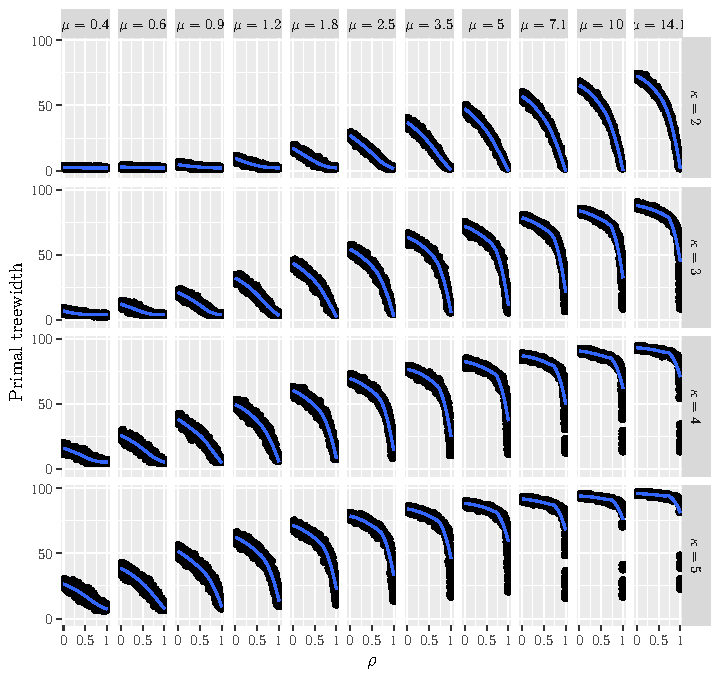
\includegraphics{chapters/comparison/regular_repetitiveness.pdf}
  \caption{The relationship between $\rho$ and primal treewidth for various
    values of $\mu$ and $\kappa$ for $k$-CNF formulas from
    \cref{exp:regular_satisfiability}. Black points represent individual
    instances, and blue lines are smoothed means computed using locally weighted
    smoothing. The values of $\mu$ are rounded to one decimal
    place.}\label{fig:regular_repetitiveness}
\end{figure}

\Cref{fig:regular_repetitiveness} shows the relationship between $\rho$ and
primal treewidth. Except for when both $\mu$ and $\kappa$ are set to very low
values (i.e., the formulas are small in both clause width and the number of
clauses), primal treewidth decreases as $\rho$ increases. This downward trend
becomes sharper as $\mu$ increases, however, not uniformly: it splits into a
roughly linear segment that approaches a horizontal line (for most values of
$\rho$) and a sharply-decreasing segment that approaches a vertical line (when
$\rho$ is close to one). Higher values of $\kappa$ seem to expedite this
transition, i.e., with a higher value of $\kappa$, a lower value of $\mu$ is
sufficient for a smooth downward curve between $\rho$ and primal treewidth to
turn into a combination of a horizontal and a vertical line. While this
behaviour may be troublesome when generating formulas with higher values of
$\mu$ (almost all of which would be unsatisfiable), the relationship between
$\rho$ and primal treewidth is excellent for generating 3-CNF formulas close to
and below the satisfiability threshold of
4.25 \citep{DBLP:journals/ai/CrawfordA96}.

Regarding satisfiability, the proportion of satisfiable 3-CNF formulas drops
from \SI{63.6}{\percent} when $\rho = 0$ to \SI{50.9}{\percent} when $\rho = 1$,
so---while $\rho$ does affect satisfiability---the effect is not significant
enough to influence our experimental setup in the next section.

% It is well-known that there is a sharp transition from satisfiable to
% unsatisfiable 3-CNF formulas at $\mu = 4.25$ regardless of the value of $\nu$
% (this is known as the \emph{satisfiability
% threshold})~\cite{DBLP:journals/ai/CrawfordA96}.

\section{Experimental Results}\label{sec:experiments}

\begin{figure}[t]
  \centering
  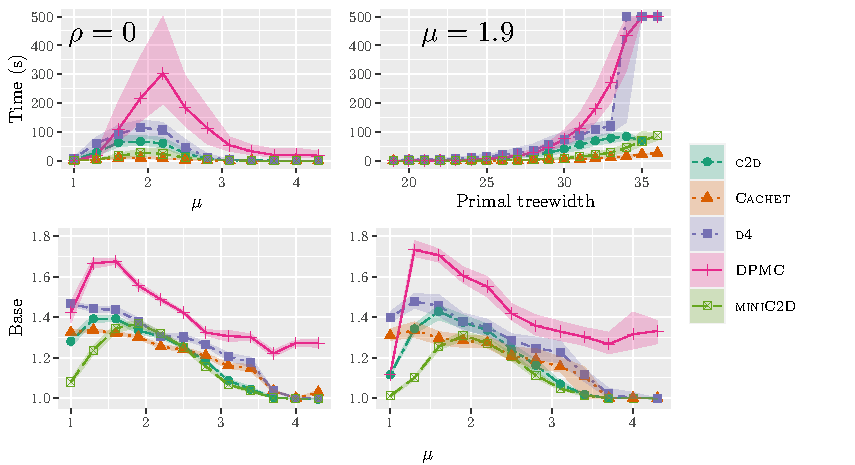
\includegraphics{chapters/comparison/treewidth}
  \caption[Visualisations of the data from \cref{exp:density}. The top-left plot
  shows how the running time of each algorithm changes w.r.t.\ density when
  $\rho = 0$. The top-right plot shows changes in the running time of each
  algorithm w.r.t.\ primal treewidth with $\mu$ fixed at $1.9$. The plots at the
  bottom show how the estimated base of the exponential relationship between
  primal treewidth and the runtime of each algorithm depends on $\mu$. The
  bottom-left plot is for the simple linear model (with shaded regions showing
  standard error), and the bottom-right plot uses the estimates provided by ESA
  (with shaded regions showing \SI{95}{\percent} confidence intervals).]%
  {Visualisations of the data from \cref{exp:density}. The top-left plot shows
    how the running time of each algorithm changes w.r.t.\ density when
    $\rho = 0$. The top-right plot shows changes in the running time of each
    algorithm w.r.t.\ primal treewidth with $\mu$ fixed at $1.9$. The plots at
    the bottom show how the estimated base of the exponential relationship
    between primal treewidth and the runtime of each algorithm depends on $\mu$.
    The bottom-left plot is for the simple linear model (with shaded regions
    showing standard error), and the bottom-right plot uses the estimates
    provided by ESA \protect{\citep{DBLP:conf/gecco/PushakH20}} (with shaded
    regions showing \SI{95}{\percent} confidence intervals).}\label{fig:treewidth}
\end{figure}

% the experimental setup
In this section, we describe three experiments that examine how the running
times of \textsf{WMC} algorithms change w.r.t.\ parameters of our random model.
All experiments were run on Intel Xeon~E5--2630 with Scientific Linux~7,
GCC~10.2.0, Python~3.8.1, R~4.1.0,
\textsc{c2d}~2.20 \citep{DBLP:conf/ecai/Darwiche04},
\textsc{Cachet}~1.22 \citep{DBLP:conf/sat/SangBBKP04},
\textsc{htd}~1.2.0 \citep{DBLP:conf/cpaior/AbseherMW17}, and with no additional preprocessing. With both \textsc{c2d} and \textsc{d4}, we use \textsc{query-dnnf}\footnote{\url{http://www.cril.univ-artois.fr/kc/d-DNNF-reasoner.html}} to compute the numerical answer from the compiled circuit. We omit \textsc{ADDMC} \citep{DBLP:conf/aaai/DudekPV20} from our experiments as it exceeds time and memory limits on too many instances; however, observations about the behaviour of \textsc{DPMC} \citep{DBLP:conf/cp/DudekPV20} apply to \textsc{ADDMC} as well, with the addendum that the tree decomposition implicitly used by \textsc{ADDMC} may have a significantly higher width. \textsc{DPMC} is run with tree decomposition-based planning (using one iteration of \textsc{htd}) and ADD-based execution---the combination that was originally found to be most effective. We restrict our attention to 3-CNF formulas, generate 100 satisfiable instances for each \emph{combination} of parameters, and run each of the five algorithms with a \SI{500}{\second} time limit and an \SI{8}{\gibi\byte} memory limit. While both limits are somewhat low, we prioritise large numbers of instances to increase the accuracy and reliability of our results. Unless stated otherwise, in each plot of this section, lines denote median values, and shaded regions show interquartile ranges. We run the following three experiments, setting $\nu = 70$ in all of them as we found that this produces instances of suitable difficulty.

\begin{experiment}[Density and Primal Treewidth]\label{exp:density}
  Let $\nu = 70$, $\mu$ go from 1 to 4.3 in steps of 0.3, $\rho$ go from 0 to
  0.5 in steps of 0.01, and $\delta = \epsilon = 0$.
\end{experiment}

\begin{experiment}[$\delta$]\label{exp:delta}
  Let $\nu = 70$, $\mu = 2.2$\footnote{\Cref{exp:density} shows this density to
    be the most challenging for \textsc{DPMC}.},
  $\rho = 0$, $\delta$ go from 0 to 1 in steps of 0.01, and $\epsilon = 0$.
\end{experiment}

\begin{experiment}[$\epsilon$]\label{exp:epsilon}
  Same as \cref{exp:delta} but with $\delta = 0$ and $\epsilon$ going from 0 to
  1 in steps of 0.01.
\end{experiment}

% c2d and d4 are the most memory-hungry
In each experiment, the proportion of algorithm runs that timed out never
exceeded \SI{3.8}{\percent}. While in \cref{exp:density} only \SI{1}{\percent}
of experimental runs ran out of memory, the same percentage was higher in
\cref{exp:delta,exp:epsilon}---10 and \SI{12}{\percent}, respectively.
\textsc{d4} \citep{DBLP:conf/ijcai/LagniezM17} and
\textsc{c2d} are the algorithms that
experienced the most issues fitting within the memory limit, accounting for
\SIrange{66}{72}{\percent} and \SIrange{28}{33}{\percent} of such instances,
respectively. We exclude the runs that terminated early due to running out of
memory from the rest of our analysis.

% Peaks w.r.t. density: DPMC different from other WMC algorithms which are
% different from #SAT algorithms
In \cref{exp:density}, we investigate how the running time of each algorithm
depends on the density and primal treewidth by varying both $\mu$ and $\rho$.
The results are in \cref{fig:treewidth}. The first thing to note is that the
peak hardness w.r.t.\ density occurs at around 1.9 for all algorithms except for
\textsc{DPMC}, which peaks at 2.2 instead.\footnote{While exact values might be hard to read from the plot, they are confirmed by numerical data.} This finding is consistent with previous work, which shows \textsc{Cachet} to peak at 1.8 \citep{DBLP:conf/sat/SangBBKP04}.\footnote{For comparison, $\#\SAT{}$ algorithms have been observed to peak at densities 1.2 and 1.5 \citep{DBLP:conf/aaai/Pehoushek00}.}

\begin{figure}[t]
  \centering
  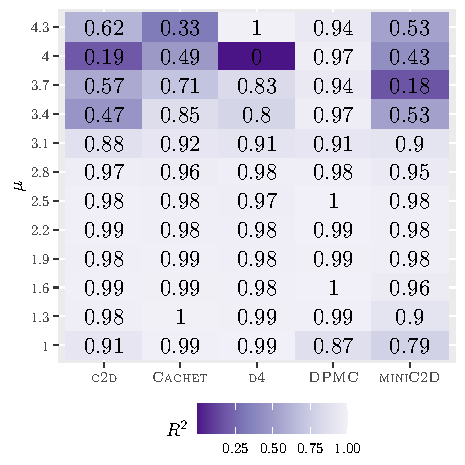
\includegraphics{chapters/comparison/r2}
  \caption{The coefficients of determination (rounded to one decimal place) of
    all the linear models fitted for the top-right subplot of
    \cref{fig:treewidth}.}\label{fig:r2}
\end{figure}

\begin{figure}[t]
  \centering
  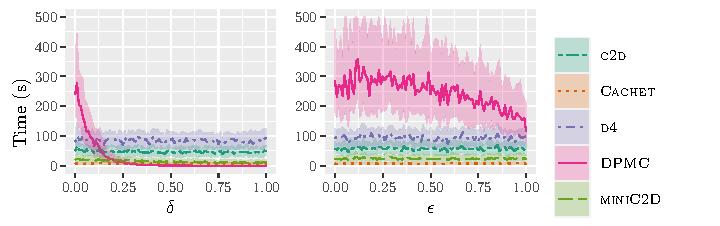
\includegraphics{chapters/comparison/delta_epsilon}
  \caption{Changes in the running time of each algorithm as a result of changing
    $\delta$ (on the left-hand side) and $\epsilon$ (on the right-hand side)
    according to the data from
    \cref{exp:delta,exp:epsilon}.}\label{fig:delta_epsilon}
\end{figure}

The other question we want to investigate using this experiment is how each algorithm scales w.r.t.\ primal treewidth. The top-right plot in \cref{fig:treewidth} shows this relationship for a fixed value of $\mu$, and one can see some evidence that the running time of \textsc{DPMC} grows faster w.r.t.\ primal treewidth than the running time of the other algorithms. We use two statistical techniques to quantify this growth: a simple linear regression model and the empirical scaling analyzer (ESA)~v2\footnote{\url{https://github.com/YashaPushak/ESA}} \citep{DBLP:conf/gecco/PushakH20}. In both cases, for each algorithm and value of $\mu$ in \cref{exp:density}, we select the median runtime for all available values of primal treewidth. In the former case, we fit the model $\ln t \sim \alpha w + \beta$, where $t$ is the median running time of the algorithm, $w$ is the primal treewidth, and $\alpha$ and $\beta$ are parameters.\footnote{Similar statistical analyses have been used to investigate polynomial-to-exponential phase transitions in \SAT{} \citep{DBLP:journals/constraints/CoarfaDASV03} and the behaviour of \SAT{} solvers on CNF-XOR formulas \citep{DBLP:conf/ijcai/DudekMV17}.} In other words, this model attempts to express median running time as $e^\beta{(e^\alpha)}^w$. In the latter case, we run ESA with 1001 bootstrap samples, a window of 101, and use the first \SI{30}{\percent} of the data for training.

% DPMC scales worse w.r.t. primal treewidth (across all densities)
The results of both models are qualitatively the same (with the exception of \textsc{DPMC} run on instances with $\mu = 1$) and are displayed at the bottom of \cref{fig:treewidth}. We find that, indeed, \textsc{DPMC} scales worse w.r.t.\ primal treewidth than any other algorithm across all values of $\mu$ and is the only algorithm that does not become indifferent to primal treewidth when faced with high-density formulas. A second look at the top-left subplot of \cref{fig:treewidth} suggests an explanation for the latter observation. The running times of all algorithms except for \textsc{DPMC} approach zero when $\mu > 3$ while the median running time of \textsc{DPMC} approaches a small non-zero constant instead. This observation also explains why \cref{fig:r2} shows that the fitted models fail to explain the data for non-ADD algorithms running on high-density instances---the running times are too small to be meaningful. In all other cases, an exponential relationship between primal treewidth and runtime fits the experimental data remarkably well.

% miniC2D is good at low-density high-primal-treewidth instances
Another thing to note is that \textsc{miniC2D} \citep{DBLP:conf/ijcai/OztokD15} is the only algorithm that exhibits a clear low-high-low pattern in the bottom subplots of \cref{fig:treewidth}. To a smaller extent, the same may apply to \textsc{c2d} and \textsc{DPMC} as well, although the evidence for this is limited due to relatively large gaps between different values of $\mu$ in \cref{exp:density}. In contrast, the running times of \textsc{Cachet} and \textsc{d4} remain dependent on primal treewidth even when the density of the \textsf{WMC} instance is very low, suggesting that \textsc{miniC2D} should have an advantage on low-density high-primal-treewidth instances.

% A median instance with all weights equal to 0.5 is about three times easier
% than a median instance with completely random weights.
Finally, \cref{exp:delta,exp:epsilon} investigate how changing the numerical values of weights can simplify a \textsf{WMC} instance. The results are in plotted \cref{fig:delta_epsilon}. As expected, the running time of all algorithms other than \textsc{DPMC} stay the same regardless of the value of $\delta$ or $\epsilon$. The running time of \textsc{DPMC}, however, experiences a sharp (exponential?) decline with increasing $\delta$. The decline w.r.t. $\epsilon$ is also present, although significantly less pronounced and with high variance.

How are these random instances different from real data? As a representative sample, we take the \textsf{WMC} encodings of Bayesian networks created using the method by \citet{DBLP:conf/aaai/SangBK05} as found in the experimental setup\footnote{\url{https://github.com/vardigroup/DPMC/releases}} of the \textsc{DPMC} paper \citep{DBLP:conf/cp/DudekPV20}. A typical \textsf{WMC} instance has $\nu = 200$ variables, half of which have equal weights (i.e., $\epsilon = 0.5$), an average clause width of $\kappa = 2.6$, a density of $\mu = 2.5$, and a primal treewidth of 28. Our random instances have fewer variables and (for the most part) lower density. Another important difference is that our instances are in $k$-CNF whereas a typical encoding of a Bayesian network has many two-literal clauses mixed with clauses of various longer widths. Despite real instances having more variables, their primal treewidth is rather low. Perhaps this partially explains why the performance of \textsc{DPMC} is in line with the performance of all other algorithms on traditionally-used benchmarks \citep{DBLP:conf/cp/DudekPV20} despite struggling with most of our random data.

To sum, we found that \textsc{c2d} and
\textsc{d4} are the most memory-intensive
algorithms, \textsc{Cachet} is great on random
instances in general, \textsc{miniC2D} exceeds
on low-density high-primal-treewidth instances, and
\textsc{DPMC} is at its best on low-density
low-primal-treewidth instances. Furthermore, a median instance with all weights
equal to each other is about three times easier for \textsc{DPMC} than a median
instance with random weights. Another important observation is about how peak
hardness w.r.t. density depends on the algorithm: \textsc{DPMC} peaks at a
higher density than all other \textsc{WMC} algorithms, which peak at a higher
density than (some) $\#\SAT{}$ algorithms.

\section{Conclusions and Future Work}

In this paper, we studied the behaviour of and differences among \textsf{WMC}
algorithms on random instances generated by a standard model for $k$-CNF
formulas extended with parameters that control primal treewidth and literal
weights. Among other things, we established statistical evidence for the
existence of an exponential relationship between primal treewidth and the
running time of all \textsf{WMC} algorithms. The running time of ADD-based
algorithms was observed to peak at a higher density, scale worse w.r.t. primal
treewidth, and depend negatively on repeating weight values compared to
algorithms based on search or knowledge compilation. These observations can, to
some degree, be extended to a closely related weighted projected model counting
algorithm \citep{DBLP:conf/sat/DudekPV21} as well as to other applications of
ADDs more generally, e.g., probabilistic
inference \citep{DBLP:conf/ijcai/ChaviraD07,DBLP:conf/uai/GogateD11} and
stochastic planning \citep{DBLP:conf/uai/HoeySHB99}.

One limitation of our work is that variability in primal treewidth was achieved
via a parameter, and this could bias randomness in some unexpected way (although
it is encouraging that there is only a slight decrease in the proportion of
satisfiable instances between $\rho=0$ and $\rho = 1$). Perhaps a theoretical
investigation of the proposed model is warranted, including a characterisation
of how $\rho$ influences primal treewidth and the structure of the primal graph
more generally. Since treewidth is widely used in parameterised complexity
\citep{DBLP:series/txcs/DowneyF13}, formally establishing a connection with
$\rho$ could make our random model useful for a variety of other hard
computational problems.

To keep the number of experiments feasible, we restricted our attention to 3-CNF
formulas, although, of course, this is not very representative of real-world
\textsf{WMC} instances. The model could be adapted to generate non-$k$-CNF
formulas, and perhaps a more representative structure could be achieved by
introducing new variables that clauses define to be equivalent to select
conjunctions of literals as is done in one of the \textsf{WMC} encodings for
Bayesian networks \citep{DBLP:conf/kr/Darwiche02}.

% It would also be interesting to see whether \textsf{WMC}
% algorithms differ in their ability to effectively handle a `shattered' solution
% space, where most solutions are distant to each other w.r.t. the Hamming
% distance \cite{DBLP:journals/rsa/AchlioptasCR11,DBLP:conf/ijcai/DudekMV17}.

\chapter{Generating Random WMC Instances} \label{chapter:comparison}

\section{Introduction}

% WMC
Weighted model counting (\textsf{WMC})---a weighted generalisation of
propositional model counting
($\#\SAT{}$) \citep{DBLP:journals/ai/ChaviraD08}---has emerged as a powerful
computational framework for problems in a variety of domains. In particular,
\textsf{WMC} has been used to perform probabilistic inference for graphical
models such as Bayesian networks and Markov random
fields \citep{DBLP:conf/ecai/BartKLM16,DBLP:conf/ijcai/ChaviraD05,DBLP:conf/sat/ChaviraD06,DBLP:conf/kr/Darwiche02,DBLP:conf/aaai/SangBK05},
probabilistic programs \citep{DBLP:journals/pacmpl/HoltzenBM20}, and
probabilistic logic programs \citep{DBLP:journals/tplp/FierensBRSGTJR15}. More
recently, \textsf{WMC} was used in the context of neural-symbolic artificial
intelligence as well \citep{DBLP:conf/icml/XuZFLB18}. Extensions of \textsf{WMC}
add support for continuous variables \citep{DBLP:conf/ijcai/BellePB15}, infinite
domains \citep{DBLP:conf/aaai/Belle17}, and first-order
logic \citep{DBLP:conf/ijcai/BroeckTMDR11,DBLP:journals/cacm/GogateD16} and
generalise the definition to support arbitrary pseudo-Boolean functions instead
of clauses \citep{DBLP:conf/sat/DilkasB21}.
Exact \textsf{WMC} algorithms can be broadly classified as based on
search \citep{DBLP:conf/sat/SangBBKP04,DBLP:conf/ijcai/SharmaRSM19}, knowledge
compilation \citep{DBLP:conf/ecai/Darwiche04,DBLP:conf/ijcai/LagniezM17,DBLP:conf/ijcai/OztokD15}, and
dynamic programming \citep{DBLP:conf/aaai/DudekPV20,DBLP:conf/cp/DudekPV20}. Other alternatives include approximate \citep{DBLP:conf/aaai/RenkensKBR14} and parallel algorithms \citep{DBLP:conf/pgm/DalLL18,DBLP:conf/esa/FichteHWZ18}, hybrid approaches \citep{DBLP:conf/sat/HecherTW20}, quantum computing \citep{DBLP:conf/ecai/Riguzzi20}, and reduction to model counting \citep{DBLP:conf/ijcai/ChakrabortyFMV15}.

% motivation for the problem
Recent papers that include experimental comparisons of \textsf{WMC}
algorithms show many of them performing very similarly
overall \citep{DBLP:conf/aaai/DudekPV20,DBLP:conf/cp/DudekPV20} but with
overwhelming differences when run on specific subsets of
data \citep{DBLP:conf/uai/DilkasB21,DBLP:conf/sat/DilkasB21,DBLP:conf/ijcai/LagniezM17}.
Examples of such segregating data sets include bipartite Bayesian networks by
\citet{DBLP:conf/aaai/SangBK05} and
relational Bayesian networks by
\citet{DBLP:journals/ijar/ChaviraDJ06}
that encode reachability in graphs under node deletion. So far, such performance
differences remain unexplained. However, knowledge about the nature of these
differences can inform our choices and aid in further algorithmic developments.
Moreover, identifying performance predictors of algorithms is often an important
step in developing a portfolio approach to the
problem \citep{DBLP:journals/jair/XuHHL08}. Lastly, if new algorithms are always
tested on the same set of benchmarks, eventually they may become somewhat fitted
to the particular characteristics of those instances, leading to algorithms that
may perform worse when run on new types of
data \citep{DBLP:conf/cec/HossainALA10}.

% related work on SAT
Both theoretical and experimental analysis of \SAT{} (and, to a lesser extent,
$\#\SAT{}$) algorithms on random instances is a rich area of research spanning
almost forty years. Variations of some of the first random models ever
proposed \citep{DBLP:journals/dam/FrancoP83,DBLP:journals/siamcomp/PurdomB83}
continue to be instrumental up to this day for, e.g., establishing the location
of the threshold between satisfiable and unsatisfiable
instances \citep{DBLP:conf/focs/AchlioptasM02} and efficiently approximating
$\#\SAT{}$ \citep{DBLP:conf/icalp/GalanisG0Y20}. Other random models consider
non-uniform variable frequencies \citep{DBLP:conf/ijcai/AnsoteguiBL09}, fixing
the number of times each variable occurs both positively and
negatively \citep{DBLP:journals/cpc/Coja-OghlanW18}, and adding other constraints
such as cardinality and `exclusive or' \citep{DBLP:conf/ijcai/PoteJM19}. In
contrast, only one \textsf{WMC} algorithm so far has been analysed using random
instances \citep{DBLP:conf/sat/SangBBKP04,DBLP:conf/sat/SangBK05}. Similarly,
while there is a recent attempt \citep{DBLP:conf/cp/DilkasB20} to compare
\textsf{WMC} algorithms on random instances of a particular application of
\textsf{WMC} (i.e., probabilistic logic programs), it fails to discern any
meaningful differences among the algorithms. The goal of this paper is to
explain some of the differences between \textsf{WMC} algorithms via an
experimental study that uses random instances.

% parameters for SAT
Experimental work investigating how \SAT{} algorithms behave on random
instances is typically centred around parameters that describe each instance
independently of its size. The most well-known parameter is the ratio of clauses
to variables (i.e., \emph{(clause) density}). Early work in the area
showed random 3-\SAT{} instances to be at their hardest when density is
around 4.25 \citep{DBLP:conf/aaai/MitchellSL92}. Later work revealed that the
interaction between density and empirical hardness is much more
solver-dependent \citep{DBLP:journals/constraints/CoarfaDASV03}. Many other
parameters such as heterogeneity, locality, and modularity have emerged from
attempts to generate random instances similar to industry benchmarks for
\SAT{} \citep{DBLP:conf/ijcai/AnsoteguiBL09,DBLP:conf/tacas/BlasiusFS19,DBLP:journals/ai/Giraldez-CruL16,DBLP:conf/ijcai/Giraldez-CruL17}.

% parameters for WMC
What parameter(s) are most appropriate to study \textsf{WMC}? Theoretical upper
bounds on the performance of various \textsf{WMC} algorithms typically include a
factor exponential in the primal treewidth of the input formula (or a closely
related
notion) \citep{DBLP:journals/jair/BacchusDP09,DBLP:journals/jacm/Darwiche01,DBLP:conf/ecai/Darwiche04,DBLP:conf/sat/SangBBKP04}.
However---as we show in \cref{sec:model}---instances generated by a standard
random model for $k$-CNF formulas fail to exhibit enough variance in primal
treewidth for us to infer its effect on the behaviour of the algorithms.
Therefore, we present an extension of this model with a parameter that
influences primal treewidth. The performance of \textsf{WMC} algorithms that use
data structures called \emph{algebraic decision diagrams}
(ADDs) \citep{DBLP:journals/fmsd/BaharFGHMPS97} is also known to depend on the
numerical values of
weights \citep{DBLP:conf/aaai/DudekPV20,DBLP:conf/cp/DudekPV20}. Thus, our random
model also includes two parameters that control redundancies in these values.
We also
investigate the effect of redundant weight values (e.g., having weights set to
zero and one or having the same weight repeat many times) on the running times
of the algorithms.

In addition to introducing a new random model for \textsf{WMC} instances, the
contributions of this paper include several key experimental findings about the
behaviour of \textsf{WMC} algorithms---namely,
\textsc{c2d}\footnote{\url{http://reasoning.cs.ucla.edu/c2d/}} \citep{DBLP:conf/ecai/Darwiche04},
\textsc{Cachet}\footnote{\url{https://cs.rochester.edu/u/kautz/Cachet/}} \citep{DBLP:conf/sat/SangBBKP04},
\textsc{d4}\footnote{\url{https://www.cril.univ-artois.fr/KC/d4.html}} \citep{DBLP:conf/ijcai/LagniezM17},
\textsc{DPMC}\footnote{\url{https://github.com/vardigroup/dpmc}} \citep{DBLP:conf/cp/DudekPV20},
and
\textsc{miniC2D}\footnote{\url{http://reasoning.cs.ucla.edu/minic2d/}} \citep{DBLP:conf/ijcai/OztokD15}---on
random instances. First, we show that the easy-hard-easy pattern with respect to
(w.r.t.) density is different for dynamic programming algorithms than it is for
all other algorithms. Second, we present statistical evidence that all the
algorithms scale exponentially w.r.t.\ primal treewidth and estimate how the
base of that exponential changes w.r.t.\ density. Third, we show how the
performance of ADD-based algorithms gradually improves w.r.t the proportion of
weights that have repeating values and sharply improves w.r.t.\ the proportion
of weights set to zero and one.

% 1. Other parameters include structural entropy
% \cite{DBLP:journals/access/LinWN21}, the proportion of clauses that have at
% most one negative literal has also been suggested as a parameter of
% interest~\cite{DBLP:journals/amai/MaarenN05}.
% 2. Maybe somewhere: relationship between primal treewidth and modularity
% 3. Just like one might choose a different propositional satisfiability
% (\SAT{}) solver based on information about the problem instance at hand (e.g.,
% `is the instance known to be satisfiable?', `was it randomly generated?', `is
% it an industrial instance?')~\cite{DBLP:journals/jair/XuHHL08},
% 4. It was also observed that replacing real numbers with addition and
% multiplication with an arbitrary commutative semiring allows \textsf{WMC} to
% subsume a variety of other problems such as most probable explanation,
% shortest path, and gradient
% computations~\cite{DBLP:journals/ijar/BelleR20,DBLP:journals/japll/KimmigBR17}.
% 5. Having these parameters in the model allows us to look not just at the
% effects of density or primal treewidth on the running times of \textsf{WMC}
% algorithms but also at the interaction between these two parameters of
% interest.

\section{Preliminaries}

% \footnote{Also known by many other names such as Gaifman, (variable)
% interaction, and variable incidence graph.}

By \emph{variable}, we always mean a Boolean variable. A \emph{literal} is
either a variable (say, $v$) or its negation (denoted $\neg v$), respectively
called \emph{positive} and \emph{negative} literal. A \emph{clause} is a
disjunction of literals. A \emph{formula} is any well-formed expression
consisting of variables, negation, conjunction, and disjunction. A formula is in
\emph{conjunctive normal form} (CNF) if it is a conjunction of clauses, and it
is in $k$-CNF if every clause has exactly $k$ literals. While we use the
set-theoretic notation for CNF formulas (e.g., writing $c \in \phi$ to mean that
clause $c$ is one of the clauses in formula $\phi$), duplicate clauses are still
allowed. The \emph{primal graph} of a CNF formula is a graph that has a node for
every variable, and there is an edge between two variables if they coappear in
some clause. The \emph{treewidth} of a graph $G$ measures how similar $G$
is to a tree and is defined as the smallest \emph{width} of any \emph{tree
  decomposition} of $G$ \citep{DBLP:journals/jct/RobertsonS84}. The \emph{primal
  treewidth} of a formula is the treewidth of its primal graph.

Given a CNF formula $\phi$, \SAT{} is a decision problem that asks whether there
exists a way to assign values to all variables in $\phi$ such that $\phi$
evaluates to true. Such a formula is said to be \emph{satisfiable}; otherwise,
it is \emph{unsatisfiable}. $\#\SAT{}$ is a problem that asks to count the
number of such assignments. \textsf{WMC} extends $\#\SAT{}$ with a weight
function on literals and asks to compute the sum of the weights of the models of
the given formula, where the weight of a model is the product of the weights of
the literals in it \citep{DBLP:journals/ai/ChaviraD08}. For example, the
\textsf{WMC} of the formula $x \lor y$ with a weight function $w\colon \{\,x, y,
\neg x, \neg y\,\} \to \mathbb{R}_{\ge 0}$ defined as $w(x) = 0.3$, $w(y) = 0.2$,
$w(\neg x) = 0.7$, $w(\neg y) = 0.8$ is $w(x)w(y)+w(x)w(\neg y)+w(\neg x)w(y) =
0.3 \times 0.2 + 0.3 \times 0.8 + 0.7 \times 0.2 = 0.44$.

\section{Background on \textsf{\textmd{WMC}} Algorithms}\label{sec:background}

In this section, we briefly review the three major approaches to \textsf{WMC}---search, knowledge compilation, and dynamic programming---and their corresponding algorithms. The main search-based \textsf{WMC} algorithm \textsc{Cachet} \citep{DBLP:conf/sat/SangBBKP04} is based on a conflict-driven clause learning \SAT{} solver \citep{DBLP:conf/dac/MoskewiczMZZM01}, which is then extended with a component caching scheme and adapted to counting.

\emph{Knowledge compilation} refers to transformations of propositional formulas
into more restrictive formats that make various operations (such as model
counting) tractable in the size of the representation
\citep{DBLP:journals/jair/DarwicheM02}.
\textsc{c2d} \citep{DBLP:conf/ecai/Darwiche04},
\textsc{d4} \citep{DBLP:conf/ijcai/LagniezM17}, and
\textsc{miniC2D} \citep{DBLP:conf/ijcai/OztokD15}
are all algorithms of this type. \textsc{c2d} compiles to deterministic
decomposable negation normal form
(d-DNNF) \citep{DBLP:journals/jancl/Darwiche01}. Similarly, \textsc{d4} compiles
to decision-DNNF (also known as decomposable decision
graphs) \citep{DBLP:conf/aaai/FargierM06}. The only difference between d-DNNF and
decision-DNNF is that decision-DNNF has if-then-else constructions instead of
disjunctions \citep{DBLP:conf/ijcai/LagniezM17}. Finally,
\textsc{miniC2D} compiles to decision-SDDs---a
subset of sentential decision diagrams (SDDs) that form a subset of
d-DNNF \citep{DBLP:conf/ijcai/Darwiche11}.

All of the algorithms mentioned above execute in exactly the same way regardless of whether computing \textsf{WMC} or $\#\SAT{}$. Two recent \textsf{WMC} algorithms instead use data structures whose size (and thus the runtime of the algorithm) depends on the numerical values of weights. These data structures are representations of \emph{pseudo-Boolean functions}, i.e., functions of the form $f\colon 2^X \to \mathbb{R}_{\ge 0}$, where $X$ is a set, and $2^X$ denotes its powerset. \textsc{ADDMC} is the first such algorithm \citep{DBLP:conf/aaai/DudekPV20}. It uses ADDs to represent pseudo-Boolean functions, combining and simplifying them in a bottom-up dynamic programming fashion. Since the size of an ADD for $f$ depends on the cardinality of the range of $f$ \citep{DBLP:journals/fmsd/BaharFGHMPS97}, the performance of the algorithm is sensitive to the numerical values of weights, e.g., to how frequently they repeat. \textsc{DPMC} extends \textsc{ADDMC} in two ways \citep{DBLP:conf/cp/DudekPV20}. First, \textsc{DPMC} allows for the order and nesting of operations on ADDs to be determined from an approximately-minimal-width tree decomposition rather than by heuristics.\footnote{There is also a recent line of work in using tree decompositions to guide the heuristics of search-based model counters \citep{DBLP:conf/cp/KorhonenJ21}.} Second, tensors are offered as an alternative to ADDs.

In all known parameterised complexities of \textsf{WMC} algorithms, the
exponential factor is a function of primal treewidth or a closely related
parameter. Interestingly, \textsc{c2d} is specifically designed to handle high
primal treewidth (which the author refers to as
\emph{connectivity} \citep{DBLP:conf/ijcai/Darwiche99}) and improves upon an
earlier algorithm that has $\mathcal{O}(mw2^w)$ time complexity, where $m$ is
the number of clauses, and $w$ is the width of the decomposition tree which is
known to be at most primal
treewidth \citep{DBLP:journals/jacm/Darwiche01,DBLP:conf/ecai/Darwiche04}. While
the complexity of \textsc{Cachet} was not analysed directly, the algorithm is
based on component caching which is known to have a
$2^{\mathcal{O}(w)}n^{\mathcal{O}(1)}$ time complexity, where $n$ is the number
of variables, and $w$ is the branchwidth of the underlying
hypergraph \citep{DBLP:journals/jair/BacchusDP09,DBLP:conf/sat/SangBBKP04}, which
is known to be within a constant factor of primal
treewidth \citep{DBLP:journals/jct/RobertsonS91}. Similarly, the complexity of
\textsf{DPMC} is not described in the paper, although the authors define a
notion of width $w$ that is at most primal treewidth plus one and estimate the
running time of the (execution part of the) algorithm to be proportional to
$2^w$ \citep{DBLP:conf/cp/DudekPV20}.

\section{Random $k$-CNF Formulas with Varying Primal
  Treewidth}\label{sec:model}

\paragraph{Notation.}
For any graph $G$, we write $\mathcal{V}(G)$ for its set of nodes and
$\mathcal{E}(G)$ for its set of edges. Let $S$ be a finite set. We write
$\mathcal{U}S$ for the discrete uniform probability distribution on $S$. We
represent any other probability distribution as a pair $(S, p)$ where $p\colon S
\to [0, 1]$ is a probability mass function. For any probability distribution
$\mathcal{P}$, we write $x \leftlsquigarrow \mathcal{P}$ to denote the act of
sampling $x$ from $\mathcal{P}$. For instance, $x \leftlsquigarrow (\{\, 1, 2 \,\}, \{\, 1 \mapsto 0.1, 2 \mapsto 0.9 \,\})$ means that $x$ becomes equal to $1$ with probability $0.1$ or to $2$ with probability $0.9$.

Our random model is based on the following parameters:
\begin{itemize}
\item the number of variables $\nu \in \mathbb{N}^+$,
\item density $\mu \in \mathbb{R}_{>0}$,
\item clause width $\kappa \in \mathbb{N}^+$ (for $k$-CNF formulas, $\kappa =
  k$),
\item a parameter $\rho \in [0, 1]$ that influences the primal treewidth of
  the formula,
\item the proportion $\delta \in [0, 1]$ of variables $x$ such that $w(x) = 1$
  and $w(\neg x) = 0$ or $w(x) = 0$ and $w(\neg x) = 1$,
\item and the proportion $\epsilon \in [0, 1-\delta]$ of variables $x$ such that
  $w(x) = w(\neg x) = 0.5$.
\end{itemize}
The first three parameters are the standard parameters used to generate random
$k$-CNF formulas with $\nu\mu$ clauses (up to rounding). We expect to observe
(possibly different) values of $\mu$ that maximize the running time of each
algorithm for fixed values of $\nu$ and $\kappa$. Parameters $\delta$ and
$\epsilon$ control the numerical values of weights and are part of the model
because the running time of \textsc{DPMC} \citep{DBLP:conf/cp/DudekPV20}---and
other algorithms based on ADDs---depends on these values. Weights such as zero
and one are particularly `simplifying' because they are respectively the
additive and multiplicative identities. Having them propagate through the
algorithm reduces the size of many ADDs used by \textsc{DPMC}, making the
algorithm more efficient. Including many copies of the same weight (e.g., 0.5)
can similarly simplify ADDs as well. Other \textsf{WMC} algorithms are
indifferent to the numerical values of weights.

\begin{algorithm}[t]
  \caption{Generating a random formula.}\label{alg:random}
  \SetKwData{kcnf}{kcnf}
  \SetKwFunction{NewVariable}{NewVariable}
  \SetKwProg{Fn}{Function}{:}{}
  \KwIn{$\nu,\kappa \in \mathbb{N}^+$ such that $\kappa < \nu$, $\mu \in
    \mathbb{R}_{>0}$, $\rho \in [0, 1]$.}
  \KwOut{A $k$-CNF formula $\phi$.}
  $\phi \gets \text{empty CNF formula}$\;
  $G \gets \text{empty graph}$\;
  \For{$i \gets 1$ \KwTo $\lfloor \nu\mu \rfloor$}{
    $X \gets \emptyset$\;
    \For{$j \gets 1$ \KwTo $\kappa$}{
      $x \gets \NewVariable{$X$, $G$}$\;
      $\mathcal{V}(G) \gets \mathcal{V}(G) \cup \{\, x \,\}$\;\label{line:7}
      $\mathcal{E}(G) \gets \mathcal{E}(G) \cup \{\, \{\,x, y\,\} \mid y \in X
      \,\}$\;\label{line:8}
      $X \gets X \cup \{\, x \,\}$\;\label{line:9}
    }
    $\phi \gets \phi \cup \{\, l \leftlsquigarrow \mathcal{U}\{\, x, \neg x \,\}
    \mid x \in X \,\}$\;\label{line:construct_clause}
  }
  \Return{$\phi$}\;
  \Fn{\NewVariable{$X$, $G$}}{
    $N \gets \{\, e \in \mathcal{E}(G) \mid |e \cap X| = 1
    \,\}$\;\label{line:13}
    \If{$N = \emptyset$}{
      \Return{$x \leftlsquigarrow \mathcal{U}(\{\, x_1, x_2, \dots, x_\nu \,\}
        \setminus X)$}\;
    }
    \nosemic\Return{$x \leftlsquigarrow \left(\{\, x_1, x_2, \dots, x_\nu \,\}
        \setminus X,\vphantom{\frac{|\{\, z \in X \mid \{\,y, z\,\} \in
            \mathcal{E}(G) \,\}|}{|N|}}\right.$}\;
      \pushline\dosemic$\left. y \mapsto \frac{1 - \rho}{\nu - |X|} +
        \rho\frac{|\{\, z \in X \mid \{\,y, z\,\} \in \mathcal{E}(G)
          \,\}|}{|N|}\right)$\; \label{line:return}
  }
\end{algorithm}

The process behind generating random $k$-CNF formulas is summarized as
\cref{alg:random}. For the rest of this section, let $x_1, x_2, \dots, x_\nu$ be
the variables of the formula under construction. We simultaneously construct
both formula $\phi$ and its primal graph $G$.\footnote{The idea to directly take
  the primal graph into consideration while generating the formula is new---cf.
  random \SAT{} instance generators based on, e.g., adversarial evolution
  \citep{DBLP:conf/cec/HossainALA10} and community structure
  \citep{DBLP:journals/ai/Giraldez-CruL16}.} Each iteration of the first for-loop
adds a clause to $\phi$. This is done by constructing a set $X$ of variables to
be included in the clause, and then randomly adding either $x$ or $\neg x$ to
the clause for each $x \in X$ on \cref{line:construct_clause}. Function
\texttt{NewVariable} randomly selects each new variable $x$, and
\cref{line:7,line:8,line:9} add $x$ to the graph and the formula while also
adding edges between $x$ and all the other variables in the clause. To select
each variable, \cref{line:13} defines set $N$ to contain all edges with exactly
one endpoint in $X$. The edges that will be added to $G$ by \cref{line:8} will
form a subset of $N$. If $N = \emptyset$, we select the variable uniformly at
random (u.a.r.) from all viable candidates. Otherwise, $\rho$ determines how
much we bias the uniform distribution towards variables that would introduce the
smallest number of new edges to $G$.

When $\rho=0$, \cref{alg:random} reduces to what has become the standard random
model for $k$-CNF formulas. Equivalently to \citet{DBLP:journals/dam/FrancoP83},
we independently sample a fixed number of clauses, each clause has no duplicate
variables, and each variable becomes either a positive or a negative literal
with equal probabilities. At the other extreme, when $\rho = 1$, the first
variable of a clause is still chosen u.a.r., but all other variables are chosen
from those that already coappear in a clause (if possible). The probability that
a variable is selected to be included in a clause scales linearly w.r.t.\ the
proportion of edges in $N$ that would be repeatedly added to $G$ if the variable
$y$ was added to the clause. This is an arbitrary choice (which appears to work
well, see \cref{sec:remarks}) although alternatives (e.g., exponential scaling)
could be considered. As long as $\rho < 1$, every $k$-CNF formula retains a
positive probability of being generated by the algorithm.

To transform the generated formula into a \textsf{WMC} instance, we need
to define weights on literals.\footnote{Note that algorithms such as
  \textsc{DPMC} and
  \textsc{ADDMC} \citep{DBLP:conf/aaai/DudekPV20,DBLP:conf/cp/DudekPV20} support
  a more flexible way of assigning weights that can lead to significant
  performance improvements \citep{DBLP:conf/uai/DilkasB21,DBLP:conf/sat/DilkasB21}.} We want to partition all variables into three groups: those with weights equal to zero and one, those with weights equal to 0.5, and those with arbitrary weights, where the size of each group is determined by $\delta$ and $\epsilon$. To do this, we sample a permutation $\pi \leftlsquigarrow \mathcal{U}S_\nu$ (where $S_\nu$ is the permutation group on $\{1, 2, \dots, \nu \}$), and assign to each \emph{variable} $x_n$ a weight drawn u.a.r.\ from
\begin{itemize}
\item $\mathcal{U}\{\,0, 1\,\}$ if $\pi(n) \le \nu\delta$,
\item $\mathcal{U}\{\,0.5\,\}$ if $\nu\delta < \pi(n) \le \nu\delta +
  \nu\epsilon$,
\item and $\mathcal{U}\{\, 0.01, 0.02, \dots, 0.99 \,\}$\footnote{For
    convenience, we represent $(0, 1)$ as 99 discrete values.} if $\pi(n) >
  \nu\delta + \nu\epsilon$.
\end{itemize}
We extend these weights to weights on \emph{literals} by choosing the weight of
each positive literal to be equal to the weight of its variable, and the weight
of each negative literal to be such that $w(x) + w(\neg x) = 1$ for all
variables $x$. This restriction is to ensure consistent answers among the
algorithms.

\begin{example}\label{example:algorithm}
  Let $\nu = 5$, $\mu = 0.6$, $\kappa = 3$, $\rho = 0.3$, $\delta = 0.4$,
  and $\epsilon = 0.2$ and consider how \cref{alg:random} generates a random
  instance. Since $\kappa = 3$, and $\lfloor\nu\mu\rfloor = 3$,
  the algorithm will generate a 3-CNF formula with three clauses.

  For the first variable of the first clause, we are choosing u.a.r.\ from $\{\,
  x_1, x_2, \dots, x_5 \,\}$. Suppose the algorithm chooses $x_5$. Graph $G$
  then gets its first node but no edges. The second variable is chosen u.a.r.
  from $\{\, x_1, x_2, x_3, x_4 \,\}$. Suppose the second variable is $x_2$.
  Then $G$ gets another node and its first edge between $x_2$ and $x_5$. The
  third variable in the first clause is similarly chosen u.a.r.\ from $\{\, x_1,
  x_3, x_4 \,\}$ because the only edge in $G$ has both endpoints in $X = \{\,
  x_2, x_5 \,\}$, and so $N = \emptyset$. Suppose the third variable is $x_1$.
  Graph $G$ becomes a triangle connecting $x_1$, $x_2$, and $x_5$. Each of
  the three variables is then added to the clause as either a positive or a
  negative literal (with equal probabilities). Thus, the first clause becomes,
  e.g., $\neg x_5 \lor x_2 \lor x_1$.

  The first variable of the second clause is chosen u.a.r.\ from $\{\, x_1, x_2,
  \dots, x_5\,\}$. Suppose it is $x_5$ again. When the function
  \texttt{NewVariable} tries to choose the second variable, $X = \{\, x_5 \,\}$,
  and so $N = \{\, \{\, x_1, x_5 \,\}, \{\, x_2, x_5 \,\}\,\}$. The second
  variable is chosen from the discrete probability distribution
  \[
    \Pr(x_1) = \Pr(x_2) = \frac{1 - 0.3}{5 - 1} + 0.3 \times \frac{1}{2} = 0.325
  \]
  and
  \[
    \Pr(x_3) = \Pr(x_4) = \frac{1 - 0.3}{5 - 1} = 0.175.
  \]

  We skip the details of how all remaining variables and clauses are selected
  and consider the weight assignment. First, we shuffle the list of variables
  and get, e.g., $L = (x_4, x_3, x_2, x_1, x_5)$. This means that the first
  $\nu\delta = 5 \times 0.4 = 2$ variables of $L$ get weights u.a.r.\ from $\{\,
  0, 1 \,\}$, the next $\nu\epsilon = 5 \times 0.2 = 1$ variable gets a weight
  of 0.5, and the remaining two variables get weights u.a.r.\ from $\{\,0.01,
  0.02, \dots, 0.99 \,\}$. The weight function $w\colon \{\, x_1, x_2, \dots,
  x_5, \neg x_1, \neg x_2, \dots, \neg x_5\,\} \to [0, 1]$ can then be defined
  as, e.g., $w(x_4) = w(\neg x_3) = 0$, $w(x_3) = w(\neg x_4) = 1$, $w(x_2) =
  w(\neg x_2) = 0.5$, $w(x_1) = 0.23$, $w(\neg x_1) = 0.77$, $w(x_5) = 0.18$,
  and $w(\neg x_5) = 0.82$.
\end{example}

% \begin{remark}
%   Note that not having a parameter that in some way influences primal treewidth
%   is unrealistic for generating instances with a wide range of primal treewidth
%   values. Without such a parameter (i.e., if $\rho=0$), the variance of primal
%   treewidth is relatively small compared to the range of values one could
%   generate by varying $\rho$ between zero and one (evidence for this is in
%   \cref{sec:remarks}).
% \end{remark}

% If all weights are different real numbers in $(0, 1)$, then performing
% addition and multiplication on them is unlikely to result in any duplicates,
% and the number of nodes in ADDs is maximised.

% i.e., the permutation $\pi$ is
% \[
%   \pi =
%   \begin{pmatrix}
%     1 & 2 & 3 & 4 & 5\\
%     4 & 3 & 2 & 1 & 5
%   \end{pmatrix}
% \]

% The novel part of the algorithm is centred around \cref{line:return}.

\subsection{Validating the Model}\label{sec:remarks}

The idea behind our model is that manipulating the value of $\rho$ should allow
us to generate instances of varying primal treewidth. Is this effect observable
in practice? In addition, as \textsf{WMC} instances are mostly used for
probabilistic inference, they tend to be satisfiable. Therefore, we want to
filter out unsatisfiable instances from those generated by the model and need to
ensure that the proportion of satisfiable instances remains sufficiently high.
Given that higher values of $\rho$ can result in constraints on variables being
more localised and concentrated, we ask: are instances generated with higher
values of $\rho$ less likely to be satisfiable? To answer both questions, we run
the following experiment.

\begin{experiment}\label{exp:regular_satisfiability}
  We fix $\nu = 100, \delta = \epsilon = 0$, and consider random instances with
  $\mu = 2.5 \times \sqrt{2}^{-5}, 2.5 \times \sqrt{2}^{-4}, \dots, 2.5 \times
  \sqrt{2}^5$, $\kappa = 2, 3, 4, 5$, and $\rho$ going from 0 to 1 in steps of
  0.01. For each combination of parameters, we generate ten instances.\footnote{Since one expects similar values of $\rho$ to produce instances with similar properties, and $\rho$'s are enumerate quite densely, generating only ten instances is sufficient.} We check if each instance is satisfiable using \textsc{MiniSat}\footnote{\url{http://minisat.se/MiniSat.html}}~2.2.0 \citep{DBLP:conf/sat/EenS03} and calculate its (approximate) primal treewidth using \textsc{htd}\footnote{\url{https://github.com/mabseher/htd}} \citep{DBLP:conf/cpaior/AbseherMW17}.
\end{experiment}

\begin{figure}[t]
  \centering
  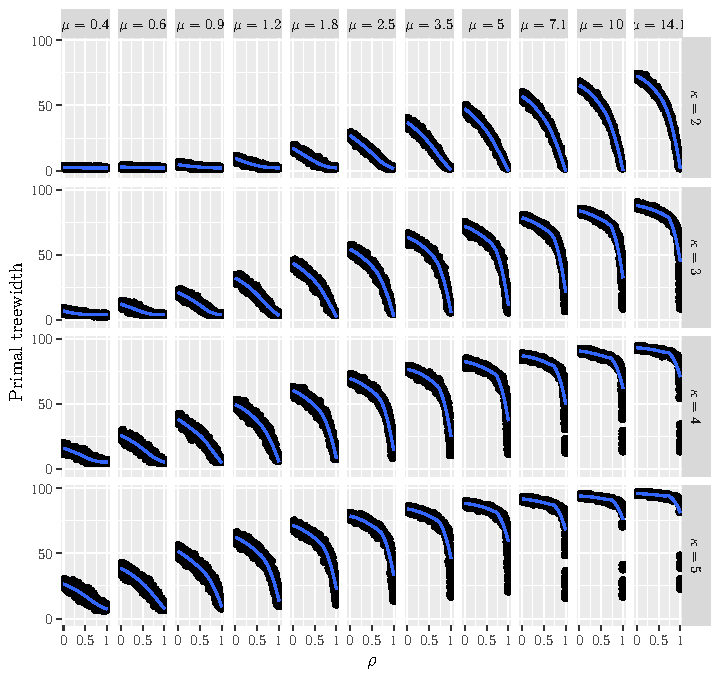
\includegraphics{chapters/comparison/regular_repetitiveness.pdf}
  \caption{The relationship between $\rho$ and primal treewidth for various
    values of $\mu$ and $\kappa$ for $k$-CNF formulas from
    \cref{exp:regular_satisfiability}. Black points represent individual
    instances, and blue lines are smoothed means computed using locally weighted
    smoothing. The values of $\mu$ are rounded to one decimal
    place.}\label{fig:regular_repetitiveness}
\end{figure}

\Cref{fig:regular_repetitiveness} shows the relationship between $\rho$ and
primal treewidth. Except for when both $\mu$ and $\kappa$ are set to very low
values (i.e., the formulas are small in both clause width and the number of
clauses), primal treewidth decreases as $\rho$ increases. This downward trend
becomes sharper as $\mu$ increases, however, not uniformly: it splits into a
roughly linear segment that approaches a horizontal line (for most values of
$\rho$) and a sharply-decreasing segment that approaches a vertical line (when
$\rho$ is close to one). Higher values of $\kappa$ seem to expedite this
transition, i.e., with a higher value of $\kappa$, a lower value of $\mu$ is
sufficient for a smooth downward curve between $\rho$ and primal treewidth to
turn into a combination of a horizontal and a vertical line. While this
behaviour may be troublesome when generating formulas with higher values of
$\mu$ (almost all of which would be unsatisfiable), the relationship between
$\rho$ and primal treewidth is excellent for generating 3-CNF formulas close to
and below the satisfiability threshold of
4.25 \citep{DBLP:journals/ai/CrawfordA96}.

Regarding satisfiability, the proportion of satisfiable 3-CNF formulas drops
from \SI{63.6}{\percent} when $\rho = 0$ to \SI{50.9}{\percent} when $\rho = 1$,
so---while $\rho$ does affect satisfiability---the effect is not significant
enough to influence our experimental setup in the next section.

% It is well-known that there is a sharp transition from satisfiable to
% unsatisfiable 3-CNF formulas at $\mu = 4.25$ regardless of the value of $\nu$
% (this is known as the \emph{satisfiability
% threshold})~\cite{DBLP:journals/ai/CrawfordA96}.

\section{Experimental Results}\label{sec:experiments}

\begin{figure}[t]
  \centering
  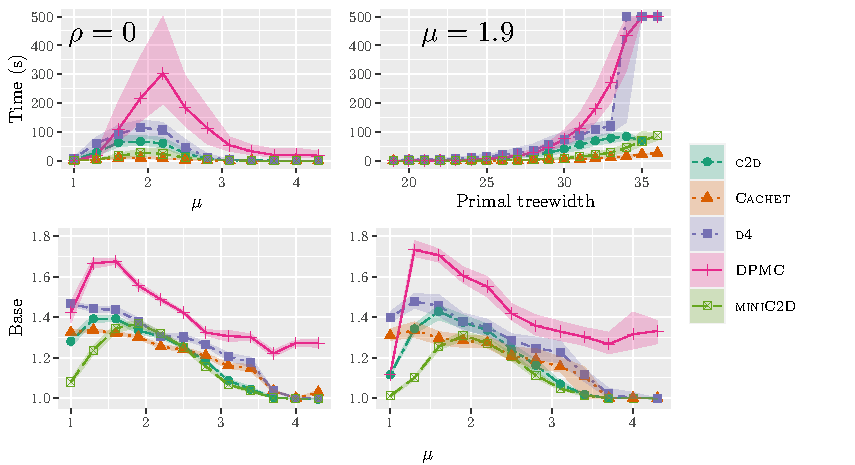
\includegraphics{chapters/comparison/treewidth}
  \caption[Visualisations of the data from \cref{exp:density}. The top-left plot
  shows how the running time of each algorithm changes w.r.t.\ density when
  $\rho = 0$. The top-right plot shows changes in the running time of each
  algorithm w.r.t.\ primal treewidth with $\mu$ fixed at $1.9$. The plots at the
  bottom show how the estimated base of the exponential relationship between
  primal treewidth and the runtime of each algorithm depends on $\mu$. The
  bottom-left plot is for the simple linear model (with shaded regions showing
  standard error), and the bottom-right plot uses the estimates provided by ESA
  (with shaded regions showing \SI{95}{\percent} confidence intervals).]%
  {Visualisations of the data from \cref{exp:density}. The top-left plot shows
    how the running time of each algorithm changes w.r.t.\ density when
    $\rho = 0$. The top-right plot shows changes in the running time of each
    algorithm w.r.t.\ primal treewidth with $\mu$ fixed at $1.9$. The plots at
    the bottom show how the estimated base of the exponential relationship
    between primal treewidth and the runtime of each algorithm depends on $\mu$.
    The bottom-left plot is for the simple linear model (with shaded regions
    showing standard error), and the bottom-right plot uses the estimates
    provided by ESA \protect{\citep{DBLP:conf/gecco/PushakH20}} (with shaded
    regions showing \SI{95}{\percent} confidence intervals).}\label{fig:treewidth}
\end{figure}

% the experimental setup
In this section, we describe three experiments that examine how the running
times of \textsf{WMC} algorithms change w.r.t.\ parameters of our random model.
All experiments were run on Intel Xeon~E5--2630 with Scientific Linux~7,
GCC~10.2.0, Python~3.8.1, R~4.1.0,
\textsc{c2d}~2.20 \citep{DBLP:conf/ecai/Darwiche04},
\textsc{Cachet}~1.22 \citep{DBLP:conf/sat/SangBBKP04},
\textsc{htd}~1.2.0 \citep{DBLP:conf/cpaior/AbseherMW17}, and with no additional preprocessing. With both \textsc{c2d} and \textsc{d4}, we use \textsc{query-dnnf}\footnote{\url{http://www.cril.univ-artois.fr/kc/d-DNNF-reasoner.html}} to compute the numerical answer from the compiled circuit. We omit \textsc{ADDMC} \citep{DBLP:conf/aaai/DudekPV20} from our experiments as it exceeds time and memory limits on too many instances; however, observations about the behaviour of \textsc{DPMC} \citep{DBLP:conf/cp/DudekPV20} apply to \textsc{ADDMC} as well, with the addendum that the tree decomposition implicitly used by \textsc{ADDMC} may have a significantly higher width. \textsc{DPMC} is run with tree decomposition-based planning (using one iteration of \textsc{htd}) and ADD-based execution---the combination that was originally found to be most effective. We restrict our attention to 3-CNF formulas, generate 100 satisfiable instances for each \emph{combination} of parameters, and run each of the five algorithms with a \SI{500}{\second} time limit and an \SI{8}{\gibi\byte} memory limit. While both limits are somewhat low, we prioritise large numbers of instances to increase the accuracy and reliability of our results. Unless stated otherwise, in each plot of this section, lines denote median values, and shaded regions show interquartile ranges. We run the following three experiments, setting $\nu = 70$ in all of them as we found that this produces instances of suitable difficulty.

\begin{experiment}[Density and Primal Treewidth]\label{exp:density}
  Let $\nu = 70$, $\mu$ go from 1 to 4.3 in steps of 0.3, $\rho$ go from 0 to
  0.5 in steps of 0.01, and $\delta = \epsilon = 0$.
\end{experiment}

\begin{experiment}[$\delta$]\label{exp:delta}
  Let $\nu = 70$, $\mu = 2.2$\footnote{\Cref{exp:density} shows this density to
    be the most challenging for \textsc{DPMC}.},
  $\rho = 0$, $\delta$ go from 0 to 1 in steps of 0.01, and $\epsilon = 0$.
\end{experiment}

\begin{experiment}[$\epsilon$]\label{exp:epsilon}
  Same as \cref{exp:delta} but with $\delta = 0$ and $\epsilon$ going from 0 to
  1 in steps of 0.01.
\end{experiment}

% c2d and d4 are the most memory-hungry
In each experiment, the proportion of algorithm runs that timed out never
exceeded \SI{3.8}{\percent}. While in \cref{exp:density} only \SI{1}{\percent}
of experimental runs ran out of memory, the same percentage was higher in
\cref{exp:delta,exp:epsilon}---10 and \SI{12}{\percent}, respectively.
\textsc{d4} \citep{DBLP:conf/ijcai/LagniezM17} and
\textsc{c2d} are the algorithms that
experienced the most issues fitting within the memory limit, accounting for
\SIrange{66}{72}{\percent} and \SIrange{28}{33}{\percent} of such instances,
respectively. We exclude the runs that terminated early due to running out of
memory from the rest of our analysis.

% Peaks w.r.t. density: DPMC different from other WMC algorithms which are
% different from #SAT algorithms
In \cref{exp:density}, we investigate how the running time of each algorithm
depends on the density and primal treewidth by varying both $\mu$ and $\rho$.
The results are in \cref{fig:treewidth}. The first thing to note is that the
peak hardness w.r.t.\ density occurs at around 1.9 for all algorithms except for
\textsc{DPMC}, which peaks at 2.2 instead.\footnote{While exact values might be hard to read from the plot, they are confirmed by numerical data.} This finding is consistent with previous work, which shows \textsc{Cachet} to peak at 1.8 \citep{DBLP:conf/sat/SangBBKP04}.\footnote{For comparison, $\#\SAT{}$ algorithms have been observed to peak at densities 1.2 and 1.5 \citep{DBLP:conf/aaai/Pehoushek00}.}

\begin{figure}[t]
  \centering
  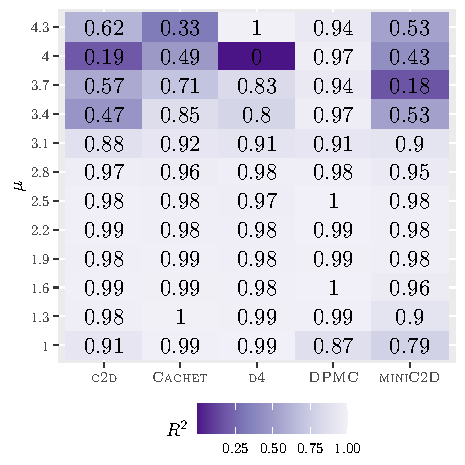
\includegraphics{chapters/comparison/r2}
  \caption{The coefficients of determination (rounded to one decimal place) of
    all the linear models fitted for the top-right subplot of
    \cref{fig:treewidth}.}\label{fig:r2}
\end{figure}

\begin{figure}[t]
  \centering
  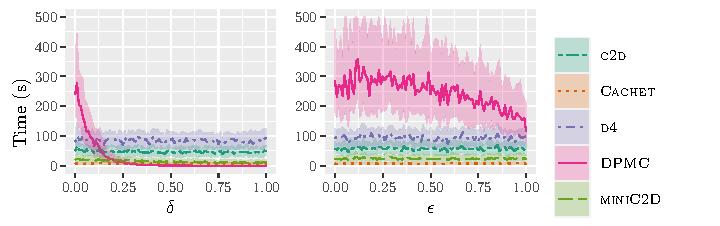
\includegraphics{chapters/comparison/delta_epsilon}
  \caption{Changes in the running time of each algorithm as a result of changing
    $\delta$ (on the left-hand side) and $\epsilon$ (on the right-hand side)
    according to the data from
    \cref{exp:delta,exp:epsilon}.}\label{fig:delta_epsilon}
\end{figure}

The other question we want to investigate using this experiment is how each algorithm scales w.r.t.\ primal treewidth. The top-right plot in \cref{fig:treewidth} shows this relationship for a fixed value of $\mu$, and one can see some evidence that the running time of \textsc{DPMC} grows faster w.r.t.\ primal treewidth than the running time of the other algorithms. We use two statistical techniques to quantify this growth: a simple linear regression model and the empirical scaling analyzer (ESA)~v2\footnote{\url{https://github.com/YashaPushak/ESA}} \citep{DBLP:conf/gecco/PushakH20}. In both cases, for each algorithm and value of $\mu$ in \cref{exp:density}, we select the median runtime for all available values of primal treewidth. In the former case, we fit the model $\ln t \sim \alpha w + \beta$, where $t$ is the median running time of the algorithm, $w$ is the primal treewidth, and $\alpha$ and $\beta$ are parameters.\footnote{Similar statistical analyses have been used to investigate polynomial-to-exponential phase transitions in \SAT{} \citep{DBLP:journals/constraints/CoarfaDASV03} and the behaviour of \SAT{} solvers on CNF-XOR formulas \citep{DBLP:conf/ijcai/DudekMV17}.} In other words, this model attempts to express median running time as $e^\beta{(e^\alpha)}^w$. In the latter case, we run ESA with 1001 bootstrap samples, a window of 101, and use the first \SI{30}{\percent} of the data for training.

% DPMC scales worse w.r.t. primal treewidth (across all densities)
The results of both models are qualitatively the same (with the exception of \textsc{DPMC} run on instances with $\mu = 1$) and are displayed at the bottom of \cref{fig:treewidth}. We find that, indeed, \textsc{DPMC} scales worse w.r.t.\ primal treewidth than any other algorithm across all values of $\mu$ and is the only algorithm that does not become indifferent to primal treewidth when faced with high-density formulas. A second look at the top-left subplot of \cref{fig:treewidth} suggests an explanation for the latter observation. The running times of all algorithms except for \textsc{DPMC} approach zero when $\mu > 3$ while the median running time of \textsc{DPMC} approaches a small non-zero constant instead. This observation also explains why \cref{fig:r2} shows that the fitted models fail to explain the data for non-ADD algorithms running on high-density instances---the running times are too small to be meaningful. In all other cases, an exponential relationship between primal treewidth and runtime fits the experimental data remarkably well.

% miniC2D is good at low-density high-primal-treewidth instances
Another thing to note is that \textsc{miniC2D} \citep{DBLP:conf/ijcai/OztokD15} is the only algorithm that exhibits a clear low-high-low pattern in the bottom subplots of \cref{fig:treewidth}. To a smaller extent, the same may apply to \textsc{c2d} and \textsc{DPMC} as well, although the evidence for this is limited due to relatively large gaps between different values of $\mu$ in \cref{exp:density}. In contrast, the running times of \textsc{Cachet} and \textsc{d4} remain dependent on primal treewidth even when the density of the \textsf{WMC} instance is very low, suggesting that \textsc{miniC2D} should have an advantage on low-density high-primal-treewidth instances.

% A median instance with all weights equal to 0.5 is about three times easier
% than a median instance with completely random weights.
Finally, \cref{exp:delta,exp:epsilon} investigate how changing the numerical values of weights can simplify a \textsf{WMC} instance. The results are in plotted \cref{fig:delta_epsilon}. As expected, the running time of all algorithms other than \textsc{DPMC} stay the same regardless of the value of $\delta$ or $\epsilon$. The running time of \textsc{DPMC}, however, experiences a sharp (exponential?) decline with increasing $\delta$. The decline w.r.t. $\epsilon$ is also present, although significantly less pronounced and with high variance.

How are these random instances different from real data? As a representative sample, we take the \textsf{WMC} encodings of Bayesian networks created using the method by \citet{DBLP:conf/aaai/SangBK05} as found in the experimental setup\footnote{\url{https://github.com/vardigroup/DPMC/releases}} of the \textsc{DPMC} paper \citep{DBLP:conf/cp/DudekPV20}. A typical \textsf{WMC} instance has $\nu = 200$ variables, half of which have equal weights (i.e., $\epsilon = 0.5$), an average clause width of $\kappa = 2.6$, a density of $\mu = 2.5$, and a primal treewidth of 28. Our random instances have fewer variables and (for the most part) lower density. Another important difference is that our instances are in $k$-CNF whereas a typical encoding of a Bayesian network has many two-literal clauses mixed with clauses of various longer widths. Despite real instances having more variables, their primal treewidth is rather low. Perhaps this partially explains why the performance of \textsc{DPMC} is in line with the performance of all other algorithms on traditionally-used benchmarks \citep{DBLP:conf/cp/DudekPV20} despite struggling with most of our random data.

To sum, we found that \textsc{c2d} and
\textsc{d4} are the most memory-intensive
algorithms, \textsc{Cachet} is great on random
instances in general, \textsc{miniC2D} exceeds
on low-density high-primal-treewidth instances, and
\textsc{DPMC} is at its best on low-density
low-primal-treewidth instances. Furthermore, a median instance with all weights
equal to each other is about three times easier for \textsc{DPMC} than a median
instance with random weights. Another important observation is about how peak
hardness w.r.t. density depends on the algorithm: \textsc{DPMC} peaks at a
higher density than all other \textsc{WMC} algorithms, which peak at a higher
density than (some) $\#\SAT{}$ algorithms.

\section{Conclusions and Future Work}

In this paper, we studied the behaviour of and differences among \textsf{WMC}
algorithms on random instances generated by a standard model for $k$-CNF
formulas extended with parameters that control primal treewidth and literal
weights. Among other things, we established statistical evidence for the
existence of an exponential relationship between primal treewidth and the
running time of all \textsf{WMC} algorithms. The running time of ADD-based
algorithms was observed to peak at a higher density, scale worse w.r.t. primal
treewidth, and depend negatively on repeating weight values compared to
algorithms based on search or knowledge compilation. These observations can, to
some degree, be extended to a closely related weighted projected model counting
algorithm \citep{DBLP:conf/sat/DudekPV21} as well as to other applications of
ADDs more generally, e.g., probabilistic
inference \citep{DBLP:conf/ijcai/ChaviraD07,DBLP:conf/uai/GogateD11} and
stochastic planning \citep{DBLP:conf/uai/HoeySHB99}.

One limitation of our work is that variability in primal treewidth was achieved
via a parameter, and this could bias randomness in some unexpected way (although
it is encouraging that there is only a slight decrease in the proportion of
satisfiable instances between $\rho=0$ and $\rho = 1$). Perhaps a theoretical
investigation of the proposed model is warranted, including a characterisation
of how $\rho$ influences primal treewidth and the structure of the primal graph
more generally. Since treewidth is widely used in parameterised complexity
\citep{DBLP:series/txcs/DowneyF13}, formally establishing a connection with
$\rho$ could make our random model useful for a variety of other hard
computational problems.

To keep the number of experiments feasible, we restricted our attention to 3-CNF
formulas, although, of course, this is not very representative of real-world
\textsf{WMC} instances. The model could be adapted to generate non-$k$-CNF
formulas, and perhaps a more representative structure could be achieved by
introducing new variables that clauses define to be equivalent to select
conjunctions of literals as is done in one of the \textsf{WMC} encodings for
Bayesian networks \citep{DBLP:conf/kr/Darwiche02}.

% It would also be interesting to see whether \textsf{WMC}
% algorithms differ in their ability to effectively handle a `shattered' solution
% space, where most solutions are distant to each other w.r.t. the Hamming
% distance \cite{DBLP:journals/rsa/AchlioptasCR11,DBLP:conf/ijcai/DudekMV17}.

\chapter{Generating Random WMC Instances} \label{chapter:comparison}

\chapter{Recursive Solutions to First-Order Model Counting} \label{chapter:wfomc}

\paragraph{Abstract.}
First-order model counting (FOMC) is a \#\P-complete computational problem that asks to count the models of a sentence in first-order logic. Despite being around for more than a decade, practical FOMC algorithms are still unable to compute functions as simple as a factorial. We argue that the capabilities of FOMC algorithms are severely limited by their inability to express arbitrary recursive computations. To enable arbitrary recursion, we relax the restrictions that typically accompany domain recursion and generalise circuits used to express a solution to an FOMC problem to graphs that may contain cycles. To this end, we enhance the most well-established (weighted) FOMC algorithm ForcLift with new compilation rules and an algorithm to check whether a recursive call is feasible. These improvements allow us to find efficient solutions to counting fundamental structures such as injections and bijections.

\clearpage
\section{Introduction/Summary}

\begin{figure}[t]
  \centering
  \begin{tikzpicture}[triangle/.style = {regular polygon, regular polygon sides=3}]
    \node[draw,ellipse] (a) at (0, 0) {$\phi(n)$};
    \node[draw,ellipse] (b) at (0, -2) {$\psi(n-1)$};
    \node[draw,ellipse] (c) at (-1, -4) {$\phi(n-1)$};
    \node[draw,triangle] (d) at (1, -4) {};
    \draw[-{Latex[length=2mm]}] (a) -- (b) node [midway,xshift=50] {domain recursion};
    \draw[-{Latex[length=2mm]}] (b) -- (c);
    \draw[-{Latex[length=2mm]}] (b) -- (d);
    \draw[-{Latex[length=2mm]}] (c) to [bend left=45] node [midway,xshift=-30] () {$n \mapsto n-1$} (a);
  \end{tikzpicture}
  \caption{An illustration of the main idea.}
  \label{fig:idea}
\end{figure}

% Definition and scope of the topic: FOMC

Need to define (W)FOMC and the logic that I'm going to use.

\begin{itemize}
\item ForcLift \citep{DBLP:conf/ijcai/BroeckTMDR11}
\item domain recursion \citep{DBLP:conf/nips/Broeck11}
\item alchemy \citep{DBLP:journals/cacm/GogateD16}
\item L2C \citep{DBLP:conf/kr/KazemiP16}
\item theory: new liftable classes \citep{DBLP:conf/nips/KazemiKBP16}
\item counting quantifiers \citep{DBLP:journals/jair/Kuzelka21}
\item tree axioms \citep{DBLP:conf/kr/BremenK21}
\item theoretical algorithm (2 variables) \citep{DBLP:conf/uai/BremenK21}
\item formula (2 variables) \citep{DBLP:journals/corr/abs-2110-05992}
\item another theoretical extension \citep{DBLP:conf/lics/KuusistoL18}
\end{itemize}

% The problem you are to focus on the topic: recursion
% If the problem was faced before, describe the state of the art.

has a similar goal \citep{DBLP:conf/ilp/BarvinekB0ZK21} BUT:

But their code only conjectures stuff. My conjectures are guaranteed always true.

They give bijection/permutation counting as an example. Are they able to find it?

But they are limited to one domain (I think...)

Another limitation: everything has to be expressible in $\mathbf{C}^2$, i.e., the two-variable fragment of first-order logic with counting quantifiers.

Data? Do they use data? Yeah, they do...

They only consider P-recursive functions, which means that, e.g., $f(n) = f(n-1)f(n-2)$ would not be allowed.

% Discuss the methods and novel techniques to be employed

\begin{itemize}
\item ForcLift \citep{DBLP:conf/ijcai/BroeckTMDR11} (first-order knowledge compilation)
\item (recursion)
\item generalising circuits to directed graphs (i.e., allowing for cycles)
\item one can then extract the (potentially recursive) definitions of functions from the graph
\item simplify the algebraic expressions, e.g.:
  \begin{itemize}
  \item adding and subtracting the same thing
  \item $\sum_{i=0}^n[i < 2]f(i) = f(0) + f(1)$
  \end{itemize}
\item evaluate the functions
\item TODO: definition of an FCG
\item maybe example of an FCG for injections
\item new compilation rules
  \begin{itemize}
  \item (generalised) domain recursion (via example)
  \item constraint removal (via example)
  \item recursion checking algorithm (sketch it)
  \end{itemize}
\item combining BFS and greedy search
\item smoothing needs to be adapted so as to not get stuck in an infinite loop
\item dynamic programming may be necessary to compute in polynomial time
\end{itemize}

% Highlights of the results obtained

able to lift most kinds of injections and bijections (same domain vs different domains AND partial vs full), e.g.:
\begin{itemize}
\item $\Theta(mn)$ for $[m] \to [n]$ injections (optimal: $\Theta(\log m)$)
\item $\Theta(m)$ for $[m] \to [n]$ bijections (optimal: $\Theta(\log m)$)
\item TODO: add/explain the formulas as well
\end{itemize}

% Possible future enhancements and further work in progress

\begin{itemize}
\item automate extracting and simplifying the definitions of functions
\item algorithm for finding all base cases
\item open questions:
  \begin{itemize}
    \item what kind of sequences are computable in this way?
    \item would using a different logic extend the capabilities of FOMC even further?
  \end{itemize}
\end{itemize}

\section{Introduction}

TODO: incorporate Vaishak's feedback (from a PDF file)

TODO: injectivity is similar to the all-different constraint

\paragraph{Differences from the propositional setting.}
\begin{itemize}
\item Propositional instances are larger, and propositional algorithms perform a large number of simple steps.
\item Heuristics, data structures, etc. matter a lot more.
\item In the FO setting, there is little data and very few steps, so it's not that important to execute each step as efficiently as possible.
\item The emphasis is more on creating new types of steps, polynomial vs exponential runtime, and maybe the degree of the polynomial.
\end{itemize}

In a way, we're dividing the idea of domain recursion between the IDR and the Ref nodes, thus also generalising it. [TODO: mention \cref{fig:idea}.]

\section{First-Order Logic}

In this section, we describe a variation of function-free first-order logic with equality. For a more complete exposition of first-order logic, see the book by \cite{DBLP:books/daglib/0023546}.

In first-order logic, an \emph{atom} (i.e., an atomic formula) is either $t_1 = t_2$ or $P(t_1, \dots, t_n)$ for some predicate $P$ and terms $(t_i)_{i=1}^n$. Here, $n \in \mathbb{N}_0$ is the \emph{arity} of $P$. A \emph{term} is either a constant or a variable (we also call terms \emph{arguments}). An atom is \emph{ground} if all of its terms are constants.

A \emph{formula} is a well-formed expression that connects atoms using the previously described logical operators as well as universal ($\forall x \in D. \phi$) and existential ($\exists x \in D. \phi$) quantifiers. Here, $x$ is a variable, $D$ is a domain, and $\phi$ is a formula. A variable occurrence is \emph{bound} if it is within the scope of a quantifier for that variable, otherwise it is \emph{free}. A formula is a \emph{sentence} if all of its variable occurrences are bound.\footnote{In the rest of this chapter, all formulas in first-order logic are assumed to be sentences.}

\subsection{How to Interpret a Sentence}

Let $\phi$ be a sentence. Since each variable in $\phi$ is introduced by a quantifier, each variable is linked to a unique domain. As is done implicitly in previous work \citep{DBLP:phd/basesearch/VandenBroeck13}, we make the following assumption.

\begin{assumption}
  Each constant can be mapped to a domain, and each $n$-ary predicate can be mapped to a sequence of $n$ domains such that:
  \begin{enumerate}
  \item ...
  \item ...
  \end{enumerate}
\end{assumption}

First, we assume that each $n$-ary predicate can be associated with a sequence of $n$ domains, one for each of its terms. Second, we assume that each constant can be similarly linked to a unique domain. Third, we assume that equality is only checked between terms that have the same domain.

TODO: describe this more formally. Maybe just two rules: whenever two terms are compared, they have the same domain, the domain of a term is always the same as the $k$-th domain of the predicate.

\begin{itemize}
\item Interpretation
  \begin{itemize}
  \item domains as sets
  \item constants as specific elements of domains (different constant implies different element. If the domain is not big enough, then the formula is unsat.)
  \item variables (indicated during quantification)
  \item predicates are interpreted as relations
  \end{itemize}
\item models are defined very differently: all combinations of relations that satisfy the sentence.
\item (multiple) (finite) domains (of discourse). This makes, e.g., satisfiability decidable and a FO formula can always be expanded to a propositional one.
\end{itemize}

more on first-order logic: \citep{DBLP:books/daglib/0023546}. The MLN paper also has a description

\section{Preliminaries}

\paragraph{Things I might need to explain.}
\begin{itemize}
\item atom, (positive/negative) literal, constant, predicate, variable, clause, unit clause, first-order logic
\item $\WMC$, $\wwp$, $\wwn$.
\item two parts: compilation and inference.
\item During inference, there is a domain size map $\size\colon \mathcal{D} \to \mathbb{N}_0$.
\item mention which rules are in $\Gamma$ and which ones are in $\Delta$ (and why tryCache has to be in $\Delta$). TODO: having notation for $\Delta$ and $\Gamma$ isn't that necessary
\item My formalisation of constraints is more restrictive than the original (e.g., in the thesis).
\item \textsc{ForcLift}
\item $\sqcup$ for both sets and functions
\end{itemize}

TODO: reorder Section 6 to introduce DR before CR before Ref.

\paragraph{Notation.}
\begin{itemize}
\item We write $\to$ for functions, $\pfun$ for partial functions, $\twoheadrightarrowtail$ for bijections, and $\hookrightarrow$ for set inclusion. Let $\id$ denote the identity function (on any domain). For any function $f$, let $\Imm f$ be the image of $f$.
\end{itemize}

Most of the definitions here are adaptations/formalisations of \cite{DBLP:conf/ijcai/BroeckTMDR11} and the corresponding code.

\begin{definition}
  A \emph{domain} is a symbol for a finite set.\footnote{In the context of functions, the domain of a function $f$ retains its usual meaning and is denoted $\dom(f)$.}
\end{definition}

\begin{definition}
  An \emph{(inequality) constraint} is a pair $(a, b)$, where $a$ is a variable, and $b$ is either a variable or a constant.
\end{definition}

\begin{definition}
  A \emph{clause} is a triple $c = (L, C, \delta_c)$, where $L$ is a set of literals, $C$ is a set of constraints, and $\delta_c$ is a function that maps all variables in $c$ to their domains such that (s.t.) if $(x, y) \in C$ for some variables $x$ and $y$, then $\delta_c(x) = \delta_c(y)$. Note that for convenience sometimes we write $\delta_c$ for the domain map of $c$ without unpacking $c$ into its three constituents.

  Also, let $\Vars$ be a function that maps clauses and sets of literals and inequalities to the set of variables contained within. In particular, $\Vars(c) \coloneqq \Vars(L) \cup \Vars(C)$.
\end{definition}

A \emph{formula} is a set of clauses. All variables in a clause are implicitly universally quantified (but note that variables are never shared among clauses), and all clauses in a formula are implicitly linked by conjunction. This way, one can read formulas as defined here as sentences in first-order logic.

TODO: Note: we will reuse this several times.
\begin{example} \label{example:first}
  Let $\phi \coloneqq \{\, c_1, c_2 \,\}$ be a formula, where
  \begin{equation} \label{phi1}
    c_1 \coloneqq (\{\, \neg p(X, Y), \neg p(X, Z) \,\}, \{\, (Y, Z) \,\}, \{\, X \mapsto a, Y \mapsto b, Z \mapsto b \,\}),
  \end{equation}
  and
  \begin{equation} \label{phi2}
    c_2 \coloneqq (\{\, \neg p(X, Y), \neg p(Z, Y) \,\}, \{\, (X, Z) \,\}, \{\, X \mapsto a, Y \mapsto b, Z \mapsto a \,\}),
  \end{equation}
  for some predicate $p$, variables $X$, $Y$, $Z$, and domains $a$ and $b$. Then in first-order logic $\phi$ could be read as
  \begin{align*}
    (\forall X \in a. \forall Y \in b. \forall Z \in b. Y \ne Z &\implies \neg p(X, Y) \lor \neg p(X, Z)) \land \\
    (\forall X \in a. \forall Y \in b. \forall Z \in a. X \ne Z &\implies \neg p(X, Y) \lor \neg p(Z, Y)).
  \end{align*}
\end{example}

\paragraph{Hashing.}
We use hash codes to efficiently check whether a recursive relationship between two formulas is plausible. (It is plausible if the formulas are equal up to variables and domains.) The hash code of a clause $c = (L, C, \delta)$ combines the hash codes of the sets of constants and predicates in $c$, the numbers of positive and negative literals, the number of inequality constraints $|C|$, and the number of variables $|\Vars(c)|$. The hash code of a formula $\phi$ combines the hash codes of all its clauses and is denoted $\#\phi$.

\paragraph{Notation for lists.}
Let $\langle\rangle$ and $\langle x \rangle$ denote an empty list and a list with one element $x$, respectively. We write $\in$ for (in-order) enumeration, $\mdoubleplus$ for concatenation, and $|\cdot|$ for the length of a list. Let $h : t$ denote a list with first element (a.k.a. head) $h$ and remaining list (a.k.a. tail) $t$. We also use list comprehensions written equivalently to set comprehensions. For example, let $L \coloneqq \langle 1 \rangle$ and $M \coloneqq \langle 2 \rangle$ be two lists. Then $M = \langle 2x \mid x \in L \rangle$, $L \mdoubleplus M = 1 : \langle 2 \rangle$, and $|M| = 1$.

\section{Generalising Circuits to Labelled Graphs}

A \emph{first-order deterministic decomposable negation normal form computational graph} (FCG) is a (weakly connected) directed graph with a a single source, vertex labels, and ordered outgoing edges.\footnote{Note that imposing an ordering on outgoing edges is just a limited version of edge labelling.} We denote an FCG as $G = (V, s, N^+, \tau)$, where $V$ is the set of vertices, and $s \in V$ is the unique source. Also, $N^+$ is the direct successor function that maps each vertex in $V$ to a \emph{list} that contains either other vertices in $V$ or a special symbol $\star$. This symbol means that the target of the edge is yet to be determined.

Vertex labels consist of two parts: the \emph{type} and the \emph{parameters}. For the main definition, we leave the parameters implicit and let $\tau\colon V \to \mathcal{T}$ denote the vertex-labelling function that maps each vertex in $V$ to its type in $\mathcal{T}$. Most of our list of types $\mathcal{T} \coloneqq \{\, \Smoothing, \Unit, \Tautology, \Contradiction, \oland, \olor, \CR, \DR, \IE, \Reff \,\}$ is as described in previous work \cite{DBLP:conf/nips/Broeck11,DBLP:conf/ijcai/BroeckTMDR11} as well as the source code of \textsc{ForcLift}\footnote{\url{https://dtai.cs.kuleuven.be/drupal/wfomc}} but with one new type $\CR$ and two revamped types $\DR$ and $\Reff$. For each vertex $v \in V$, the length of the list $N^+(v)$ (i.e., the out-degree of $v$) is determined by its type $\tau(v)$.

TODO: conjunctions and disjunctions should be different from set-conjunctions and set-disjunctions.

As in previous work \cite{DBLP:conf/ijcai/BroeckTMDR11}, to describe individual vertices and small (sub)-FCGs, we also use notation of the form, e.g., $\Reff_\rho(v)$. Here, the type of the vertex (e.g., $\Reff$) is `applied' to its direct successors (e.g., $v$) using either function or infix notation and provided with its parameter(s) (e.g., $\rho$) in the subscript. We say that `$G$ is an FCG for formula $\phi$' if two conditions are satisfied. First, the image of $N^+$ contains no $\star$'s. Second, $G$ encodes a function that maps the sizes of the domains in $\phi$ to the WMC of $\phi$ (more on this in \cref{sec:evaluation}).

\paragraph{TODO.}
\begin{itemize}
\item provide a short explanation of the types (emphasising which ones are new/updated). %\footnote{The new (as well as significantly renewed) types in \mathcal{T} are described in subsequent (TODO: which ones?) sections. The meanings of other types are described...}
\item have an example of a simple FCG. Maybe describe the figure from later and move it here.
\end{itemize}

\section{Compilation as Search}

\begin{definition}
  A \emph{state} (of the search for an FCG for a given formula) is a tuple $(G, C, L)$, where:
  \begin{itemize}
  \item $G$ is an FCG (or \texttt{null}),
  \item $C$ is a compilation cache that maps integers to sets of pairs $(\phi, v)$, where $\phi$ is a formula, and $v$ is a vertex of $G$ (which is used to identify opportunities for recursion),
  \item and $L$ is a list of formulas (that are yet to be compiled). (Note that the order is crucial!)
  \end{itemize}
\end{definition}

\begin{definition}
  A (compilation) \emph{rule} is a function that takes a formula and returns a set of $(G, L)$ pairs, where $G$ is a (potentially \texttt{null}) FCG, and $L$ is a list of formulas.

  TODO: Take the example from the AIAI talk.
\end{definition}

We assume that if there is a pair $(\texttt{null}, L)$ in the set returned by a rule, then $|L| = 1$, i.e., the rule transformed the formula without creating any vertices.

\begin{algorithm}[t]
  \caption{The (main part of the) search algorithm}
  \label{alg:search}
  \SetKwProg{Fn}{Function}{:}{}
  \SetKwData{solutions}{solutions}
  \SetKwFunction{applyGreedyRules}{applyGreedyRules}
  \SetKwFunction{applyAllRules}{applyAllRules}
  \SetKwFunction{put}{put}
  \SetKwFunction{get}{get}
  \SetKwFunction{emptyy}{empty}
  \KwIn{a formula $\phi_0$}
  \KwOut{all found FCGs for $\phi_0$ are in the set \solutions}
  $\solutions \gets \emptyset$\;
  $C_0 \gets \emptyset$\;
  $(G_0, C_0, L_0) \gets \applyGreedyRules{$\phi_0$, $C_0$}$\;
  \lIf{$L_0 = \langle\rangle$}{$\solutions \gets \{\, G_0 \,\}$}
  \Else{
    $q \gets \text{an empty queue of states}$\;
    $q.\put{$(G_0, C_0, L_0)$}$\;
    \While{{\bf not} $q.\emptyy{}$}{
      \ForEach{state $(G, C, L) \in \applyAllRules{$q.\get{}$}$}{
        \lIf{$L = \langle\rangle$}{$\solutions \gets \solutions \cup \{\, G \,\}$}
        \lElse{$q.\put{$(G, C, L)$}$}
      }
    }
  }
\end{algorithm}

\begin{algorithm}
  \caption{Functions used in \cref{alg:search} for applying compilation rules}
  \label{alg:apply}
  \SetKwProg{Fn}{Function}{:}{}
  \SetKwData{newStates}{newStates}
  \SetKwFunction{applyGreedyRules}{applyGreedyRules}
  \SetKwFunction{applyAllRules}{applyAllRules}
  \SetKwFunction{applyGreedyRulesToAllFormulas}{applyGreedyRulesToAllFormulas}
  \SetKwFunction{mergeFcgs}{mergeFcgs}
  \SetKwFunction{updateCache}{updateCache}
  \KwData{a set of greedy rules $\Gamma$}
  \KwData{a set of non-greedy rules $\Delta$}
  \Fn{\applyGreedyRules{$\phi$, $C$}}{
    \ForEach{rule $r \in \Gamma$}{
      \If{$r(\phi) \ne \emptyset$}{
        $(G, L) \gets \text{any element of } r(\phi)$\;
        \lIf{$G = {\normalfont \texttt{null}}$}{\Return{\applyGreedyRules{the only element of $L$, $C$}}}
        \Else{
          $(V, s, N^+, \tau) \gets G$\;
          $C \gets \updateCache{$C$, $\phi$, $G$}$\;
          \Return{\applyGreedyRulesToAllFormulas{$G$, $C$, $L$}}\;
        }
      }
    }
    \Return{$({\normalfont \texttt{null}}, C, \langle\phi\rangle)$}\;
  }
  \Fn{\applyGreedyRulesToAllFormulas{$(V, s, N^+, \tau)$, $C$, $L$}}{
    \lIf{$L = \langle\rangle$}{\Return{$((V, s, N^+, \tau), C, L)$}}
    $N^+(s) \gets \langle\rangle$\;
    $L' \gets \langle\rangle$\;
    \ForEach{formula $\phi \in L$}{
      $(G', C, L'') \gets \applyGreedyRules{$\phi$, $C$}$\;
      $L' \gets L' \mdoubleplus L''$\;
      \lIf{$G' = {\normalfont \texttt{null}}$}{$N^+(s) \gets N^+(s) \mdoubleplus \langle\star\rangle$}
      \Else{
        $(V', s', N', \tau') \gets G'$\;
        $V \gets V \sqcup V'$\;
        $N^+ \gets N^+ \sqcup N'$\;
        $N^+(s) \gets N^+(s) \mdoubleplus \langle s' \rangle$\;
        $\tau \gets \tau \sqcup \tau'$\;
      }
    }
    \Return{$((V, s, N^+, \tau), C, L')$}\;
  }
  \Fn{\applyAllRules{$s$}}{
    $(G, C, L) \gets s$\;
    $\phi : T \gets L$\;
    $(G', C', L') \gets \text{a copy of } s$\;
    $\newStates \gets \langle\rangle$\;
    \ForEach{rule $r \in \Delta$}{
      \ForEach{$(G'', L'') \in r(\phi)$}{
        \lIf{$G'' = {\normalfont \texttt{null}}$}{$\newStates \gets \newStates \mdoubleplus \applyAllRules{$(G', C', L'')$}$}
        \Else{
          $(V, s, N^+, \tau) \gets G''$\;
          $C' \gets \updateCache{$C'$, $\phi$, $G''$}$\;
          $(G'', C', L'') \gets \applyGreedyRulesToAllFormulas{$G''$, $C'$, $L''$}$\;
          \lIf{$G' = {\normalfont \texttt{null}}$}{$\newStates \gets \newStates \mdoubleplus \langle(G'', C', L'' \mdoubleplus T)\rangle$}
          \lElse{$\newStates \gets \newStates \mdoubleplus \langle(\mergeFcgs{$G'$, $G''$}, C', L'' \mdoubleplus T)\rangle$}
        }
      }
      $(G', C', L') \gets \text{a copy of } s$\;
    }
    \Return{\newStates}\;
  }
\end{algorithm}

\begin{algorithm}
  \caption{Helper functions used by \cref{alg:apply}}
  \label{alg:helpers}
  \SetKwProg{Fn}{Function}{:}{}
  \SetKwFunction{mergeFcgs}{mergeFcgs}
  \SetKwFunction{updateCache}{updateCache}
  \Fn{\updateCache{$C$, $\phi$, $(V, s, N^+, \tau)$}}{
    \lIf{$\tau(s) = \textsc{Ref}$}{\Return{$C$}}
    \lIf{$\#\phi \not\in \dom(C)$}{\Return{$C \cup \{\, \#\phi \mapsto (\phi, s) \,\}$}}
    \lIf{there is no $(\phi', v) \in C(\#\phi)$ s.t. $v = s$}{$C(\#\phi) \gets (\phi, s) \mdoubleplus C(\#\phi)$}
    \Return{$C$}\;
  }
  \Fn{\mergeFcgs{$G = (V, s, N^+, \tau)$, $G' = (V', s', N', \tau')$, $r = s$}}{
    \lIf{$\tau(r) = \textsc{Ref}$}{\Return{\normalfont \texttt{null}}}
    \ForEach{$t \in N^+(r)$}{
      \If{$t = \star$}{
        replace $t$ with $s'$ in $N^+(r)$\;
        \Return{$(V \sqcup V', s, N^+ \sqcup N', \tau \sqcup \tau')$}\;
      }
      $G'' \gets \mergeFcgs{$G$, $G'$, $t$}$\;
      \lIf{$G'' \ne {\normalfont \texttt{null}}$}{\Return{$G''$}}
    }
    \Return{\normalfont \texttt{null}}\;
  }
\end{algorithm}

TODO: explain the `tail' part of the algorithm, i.e., that the first formula is replaced by some vertices and some formulas. And explain why we don't want to have \textsc{Ref} vertices in the cache.

Note: At the end, \texttt{mergeFcgs} will never return \texttt{null} because there is going to be at least one $\star$ in $G$ and the function will find it.

\section{In-Between Compilation and Inference: Smoothing}

\begin{algorithm}
  \SetKwData{changed}{changed}
  \caption{Propagating atoms for smoothing across the FCG in a way that avoids infinite loops}
  \label{alg:smoothing}
  \KwIn{FCG $(V, s, N^+, \tau)$}
  \KwIn{function $\iota$ that maps vertex types in $\mathcal{T}$ to sets of atoms}
  \KwIn{functions $\{\,f_t\,\}_{t \in \mathcal{T}}$ that take a list of sets of atoms and return a set of atoms}
  \KwOut{function $S$ that maps vertices in $V$ to sets of atoms}
  $S \gets \{\, v \mapsto \iota(\tau(v)) \mid v \in V \,\}$\;
  $\changed \gets \texttt{true}$\;
  \While{\changed}{
    $\changed \gets \texttt{false}$\;
    \ForEach{vertex $v \in V$}{
      $S' \gets f_{\tau(v)}(\langle S(w) \mid w \in N^+(v) \rangle)$\;
      \If{$S' \ne S(v)$}{
        $\changed \gets \texttt{true}$\;
        $S(v) \gets S'$\;
      }
    }
  }
\end{algorithm}

[Insert motivation for smoothing from Section 3.4. of the ForcLift paper.] Originally, smoothing was (and still is) a two-step process. First, atoms that are still accounted for in the circuit are propagated upwards. Then, at vertices of certain types, missing atoms are detected and additional sinks are created to account for them. If left unchanged, the first step of this process would result in an infinite loop whenever a cycle is encountered. \Cref{alg:smoothing} outlines how the first step can be adapted to an arbitrary directed graph.

\section{New Compilation Rules}

Let $\mathcal{D}$ be the set of all domains. Note that this set expands during the compilation.

\subsection{Identifying Possibilities for Recursion}

\subsubsection{Notation}

Let $\Doms$ be a function that maps any clause or formula to the set of domains used within. Specifically, $\Doms(c) \coloneqq \Imm \delta_c$ for any clause $c$, and $\Doms(\phi) \coloneqq \bigcup_{c \in \phi} \Doms(c)$ for any formula $\phi$.

For partial functions $\alpha, \beta\colon A \pfun B$ s.t. $\alpha|_{\dom(\alpha) \cap \dom(\beta)} = \beta|_{\dom(\alpha) \cap \dom(\beta)}$, we write $\alpha \cup \beta$ for the unique partial function s.t. $\alpha \cup \beta|_{\dom(\alpha)} = \alpha$, and $\alpha \cup \beta|_{\dom(\beta)} = \beta$.

For any clause $c = (L, C, \delta_c)$, bijection $\beta\colon \Vars(c) \twoheadrightarrowtail V$ (for some set of variables $V$), and function $\gamma\colon \Doms(c) \to \mathcal{D}$, let $c[\beta, \gamma] = d$ be the clause $c$ with all occurrences of any variable $v \in \Vars(c)$ in $L$ and $C$ replaced with $\beta(v)$ (so $\Vars(d) = V$) and $\delta_d\colon V \to \mathcal{D}$ defined as $\delta_d \coloneqq \gamma \circ \delta_c \circ \beta^{-1}$. In other words, $\delta_d$ is the unique function that makes
\[
\begin{tikzcd}
  \Vars(c) \ar[r, tail, two heads, "\beta"] \arrow[d, swap, "\delta_c"] & V = \Vars(d) \ar[d, dashed, "\exists!\delta_d"] \\
  \Doms(c) \ar[r, swap, "\gamma"] & \mathcal{D}
\end{tikzcd}
\]
commute. For example, if clause $c_1$ is as in \cref{example:first}, then
\begin{multline*}
  c_1[\{\, X \mapsto A, Y \mapsto B, Z \mapsto C \,\}, \{\, a \mapsto b, b \mapsto c \,\}] = \\
  (\{\, \neg p(A, B), \neg p(A, C) \,\}, \{\, (B, C) \,\}, \{\, A \mapsto b, B \mapsto c, C \mapsto c \,\}).
\end{multline*}

\subsubsection{Everything Else}

\begin{algorithm}[t]
  \caption{The compilation rule for $\Reff$}
  \label{alg:trycache}

  \SetKwProg{Fn}{Function}{:}{}
  \SetKw{KwRet}{yield}
  \SetKwData{compilationCache}{compilationCache}
  \SetKwFunction{identifyRecursion}{identifyRecursion}
  \SetKwFunction{generateMaps}{generateMaps}
  \SetKwFunction{constructDomainMap}{constructDomainMap}

  \KwIn{formula $\phi$}
  \KwOut{either a singleton with the new $\Reff$ vertex or $\emptyset$}

  \ForEach{$(\psi, v) \in \compilationCache{$\#\phi$}$}{
    $\rho \gets \identifyRecursion{$\phi$, $\psi$}$\;
    \lIf{$\rho \ne {\normalfont \texttt{null}}$}{\Return{$\{\, (\Reff_\rho(v), \emptyset) \,\}$}}
  }
  \Return{$\emptyset$}\;

  \Fn{\identifyRecursion{$\phi$, $\psi$, $\rho = \emptyset$}}{
    \lIf{$|\phi| \ne |\psi|$ {\bf or} $\#\phi \ne \#\psi$}{\Return{\normalfont \texttt{null}}}
    \lIf{$\phi = \emptyset$}{\Return{$\rho$}}
    \ForEach{clause $c \in \phi$\label{line:for1}}{
      \ForEach{clause $d \in \psi$ s.t. $\#d = \#c$\label{line:for2}} {
        \ForEach{$(\beta, \gamma) \in \generateMaps{$c$, $d$, $\rho$}$ s.t. $c[\beta, \gamma] = d$\label{line:generateMaps}}{
          $\rho' \gets \identifyRecursion{$\phi \setminus \{\, c \,\}$, $\psi \setminus \{\, d \,\}$, $\rho \cup \gamma$}$\;\label{line:recursion}
          \lIf{$\rho' \ne {\normalfont \texttt{null}}$}{\Return{$\rho'$}}
        }
      }
      \Return{\normalfont \texttt{null}}\;
    }
  }

  \Fn{\generateMaps{$c$, $d$, $\rho$}}{
    \ForEach{bijection $\beta\colon \Vars(c) \to \Vars(d)$\label{line:bijection}}{
      $\gamma \gets \constructDomainMap{$\Vars(c)$, $\delta_c$, $\delta_d$, $\beta$, $\rho$}$\;
      \lIf{$\gamma \ne {\normalfont \texttt{null}}$}{\KwRet{$(\beta, \gamma)$}}
    }
  }

  \Fn{\constructDomainMap{$V$, $\delta_c$, $\delta_d$, $\beta$, $\rho$}}{
    $\gamma \gets \emptyset$\;
    \ForEach{$v \in V$}{
      \lIf{$\delta_c(v) \in \dom(\rho)$ {\bf and} $\rho(\delta_c(v)) \ne \delta_d(\beta(v))$}{\Return{\normalfont \texttt{null}}}
      \lIf{$\delta_c(v) \not\in \dom(\gamma)$}{$\gamma \gets \gamma \cup \{\, \delta_c(v) \mapsto \delta_d(\beta(v)) \,\}$}
      \lElseIf{$\gamma(\delta_c(v)) \ne \delta_d(\beta(v))$}{\Return{\normalfont \texttt{null}}}
    }
    \Return{$\gamma$}\;
  }
\end{algorithm}

\paragraph{TODO}
\begin{itemize}
\item introduce/describe \cref{alg:trycache} and describe the cache that's being used.
\item explain why $\rho \cup \gamma$ is possible
\item explain what the second return statement is about and why a third one is not necessary
\item explain the yield keyword
\item in the example below: write down both formula using the ForcLift format
\end{itemize}

The algorithm could be improved in two ways:
\begin{itemize}
\item by constructing a domain map first and then using it to reduce the number of viable variable bijections.
\item by similarly using the domain map $\rho$.
\end{itemize}
However, it is not clear that this would result in an overall performance improvement, since the number of variables in instances of interest never exceeds three and the identity bijection is typically the right one.

Diagramatically, \texttt{constructDomainMap} attempts to find $\gamma\colon \Doms(c) \to \Doms(d)$ s.t.
\begin{equation} \label{eq:commute}
\begin{tikzcd}
  \Vars(c) \ar[r, tail, two heads, "\beta"] \arrow[d, swap, "\delta_c"] & \Vars(d) \ar[d, "\delta_d"] \\
  \Doms(c) \ar[r, dashed, "\gamma"] \ar[d, hookrightarrow] & \Doms(d) \ar[d, hookrightarrow] \\
  \mathcal{D} \ar[r, swap, "\rho"] & \mathcal{D}.
\end{tikzcd}
\end{equation}
commutes (and returns \texttt{null} if such a function does not exist).

TODO: update this example. Fix references.
\begin{example} \label{example}
  Let $\phi$ be the formula from \cref{example:first} and $\psi \coloneqq \phi[\id, \{\, a \mapsto a', b \mapsto b^\bot \,\}]$ (i.e., $\phi$ with both of its domains replaced). Since $\#\phi = \#\psi$, and both formulas are non-empty, the algorithm proceeds with the for-loops on \cref{line:for1,line:for2,line:generateMaps}. Suppose $c$ in the algorithm refers to \cref{phi1}, and $d$ to \cref{psi1}. Since both clauses have three variables, in the worst case, function \texttt{generateMaps} would have $3!=6$ bijections to check. Suppose the identity bijection is picked first. Then \texttt{constructDomainMap} is called with the following parameters:
  \begin{itemize}
  \item $V = \{\, X, Y, Z \,\}$,
  \item $\delta_c = \{\, X \mapsto a, Y \mapsto b, Z \mapsto b \,\}$,
  \item $\delta_d = \{\, X \mapsto a', Y \mapsto b^\bot, Z \mapsto b^\bot \,\}$,
  \item $\beta = \{\, X \mapsto X, Y \mapsto Y, Z \mapsto Z \,\}$,
  \item $\rho = \emptyset$.
  \end{itemize}
  Since $\delta_i(Y) = \delta_i(Z)$ for $i \in \{\, c, d \,\}$, \texttt{constructDomainMap} returns $\gamma = \{\, a \mapsto a', b \mapsto b^\bot \,\}$. Thus, \texttt{generateMaps} yields its first pair of maps $(\beta, \gamma)$ to \cref{line:generateMaps}. Furthermore, the pair satisfies $c[\beta, \gamma] = d$.

  Since $\pi(a') = a$, and $a' \in \mathcal{C}$, \texttt{traceAncestors($a$, $a'$)} returns \texttt{true}, which sets $\textsf{foundConstraintRemoval}'$ to \texttt{true} as well. When $e = b$, however, \texttt{traceAncestors}($b$, $b^\bot$) returns \texttt{false} since $b^\bot$ is a descendant of $b$ but not created by the constraint removal compilation rule. On \cref{line:recursion}, a recursive call to \texttt{identifyRecursion($\phi'$, $\psi'$, $\gamma$, true)} is made, where $\phi'$ and $\psi'$ are new formulas with one clause each: \cref{phi2} and \cref{psi2}, respectively.

  Again we have two non-empty formulas with equal hash codes, so \texttt{generateMaps} is called with $c$ set to \cref{phi2}, $d$ set to \cref{psi2}, and $\rho = \{\, a \mapsto a', b \mapsto b^\bot \,\}$. Suppose \cref{line:bijection} picks the identity bijection first again. Then \texttt{constructDomainMap} is called with the following parameters:
  \begin{itemize}
  \item $V = \{\, X, Y, Z \,\}$,
  \item $\delta_c = \{\, X \mapsto a, Y \mapsto b, Z \mapsto a \,\}$,
  \item $\delta_d = \{\, X \mapsto a', Y \mapsto b^\bot, Z \mapsto a' \,\}$,
  \item $\beta = \{\, X \mapsto X, Y \mapsto Y, Z \mapsto Z \,\}$,
  \item $\rho = \{\, a \mapsto a', b \mapsto b^\bot \,\}$.
  \end{itemize}
  Since $\beta$ and $\rho$ commute (as in \cref{eq:commute}), and there are no new domains in $\Doms(c)$ and $\Doms(d)$, $\gamma$ exists and is equal to $\rho$. Again, the returned pair $(\beta, \gamma)$ satisfies $c[\beta, \gamma] = d$. \Cref{line:recursion} calls \texttt{identifyRecursion($\emptyset$, $\emptyset$, $\rho$, true)}, which immediately returns $\rho = \{\, a \mapsto a', b \mapsto b^\bot \,\}$ as the final answer. This means that one can indeed use an FCG for $\WMC(\phi)$ to compute $\WMC(\psi)$ by replacing every mention of $a$ with $a'$ and every mention of $b$ with $b^\bot$.
\end{example}

\subsubsection{Evaluation}

$\WMC(\Reff_\rho(v); \size) = \WMC(v; \size')$ ($n$ is the target vertex), where $\size'$ is defined as
\[
\size'(x) =
\begin{cases}
  \size(\rho(x)) & \text{if } x \in \dom(\rho) \\
  \size(x) & \text{otherwise}
\end{cases}
\]
for all $x \in \mathcal{D}$.

\subsection{Constraint Removal}

\begin{algorithm}[t]
  \caption{The compilation rule for $\CR$}
  \label{alg:constraintremoval}
  \KwIn{formula $\phi$, set of domains $\mathcal{D}$}
  \KwOut{set $S$}
  $S \gets \emptyset$\;
  \ForEach{domain $d \in \mathcal{D}$ and element $e \in d$ s.t. $e$ does not occur in any literal of any clause of $\phi$ {\bf and} for each clause $ c = (L, C, \delta_c) \in \phi$ and variable $v \in \Vars(c)$, either $\delta_c(v) \ne d$ {\bf or} $(v, e) \in C$}{
    add a new domain $d'$ to $\mathcal{D}$\;
    $\phi' \gets \emptyset$\;
    \ForEach{clause $(L, C, \delta) \in \phi$}{
      $C' \gets \{\, (x, y) \in C \mid y \ne e \,\}$\;
      $\delta' \gets \emptyset$\;
      \ForEach{variable $v \in \Vars(L) \cup \Vars(C')$}{
        \lIf{$\delta(v) = d$}{$\delta' \gets \delta' \cup \{\, v \mapsto d' \,\}$}
        \lElse{$\delta' \gets \delta' \cup \{\, v \mapsto \delta(v) \,\}$}
      }
      $\phi' \gets \phi' \cup \{\, (L, C', \delta') \,\}$\;
    }
    $S \gets S \cup \{\, \CR_{d \mapsto d'}, \phi' \,\}$\;
  }
\end{algorithm}

TODO: describe \cref{alg:constraintremoval} and rewrite the example below.

\begin{example}
  Let $\phi = \{\, c_1, c_2, c_e \,\}$ be a formula with clauses (constants lowercase, variables uppercase)
  \begin{align*}
    c_1 &= (\emptyset, \{\, (Y, X) \,\}, \{\, X \mapsto b^\top, Y \mapsto b^\top \,\}), \\
    c_2 &= (\{\, \neg p(X, Y), \neg p(X, Z) \,\}, \{\, (X, x), (Y, Z) \,\}, \{\, X \mapsto a, Y \mapsto b^\bot, Z \mapsto b^\bot \,\}), \\
    c_3 &= (\{\, \neg p(X, Y), \neg p(Z, Y) \,\}, \{\, (X, x), (Z, X), (Z, x) \,\}, \{\, X \mapsto a, Y \mapsto b^\bot, Z \mapsto a \,\}).
  \end{align*}
  Domain $a$ and with its element $x \in a$ satisfy the preconditions for constraint removal. The operator introduces a new domain $a'$ and transforms $\phi$ to $\phi' = (c_1', c_2', c_3')$, where
  \begin{align*}
    c_1' &= c_1 \\
    c_2' &= (\{\, \neg p(X, Y), \neg p(X, Z) \,\}, \{\, (Y, Z) \,\}, \{\, X \mapsto a', Y \mapsto b^\bot, Z \mapsto b^\bot \,\}) \\
    c_3' &= (\{\, \neg p(X, Y), \neg p(Z, Y) \,\}, \{\, (Z, X) \,\}, \{\, X \mapsto a', Y \mapsto b^\bot, Z \mapsto a' \,\}).
  \end{align*}
\end{example}

\paragraph{Evaluation.}
\[
\WMC(\CR_{d \mapsto d'}(n); \size) =
\begin{cases}
  \WMC(n; \size \cup \{\, d' \mapsto \size(d) - 1 \,\}) & \text{if } \size(d) > 0 \\
  0 & \text{otherwise.}
\end{cases}
\]

\subsection{A Generalisation of Domain Recursion}

\begin{algorithm}[t]
  \caption{The compilation rule for $\DR$}
  \label{alg:domainrecursion}
  \KwIn{formula $\phi$}
  \KwOut{set $S$}
  $S \gets \emptyset$\;
  \ForEach{domain $d \in \mathcal{D}$ s.t. there is a clause $c \in \phi$ and a variable $v \in \Vars(L_c)$ s.t. $\delta_c(v) = d$}{
    $\phi' \gets \emptyset$\;
    $x \gets \text{a new constant associated with domain } d$\;
    \ForEach{clause $c = (L, C, \delta) \in \phi$\label{line:forclause}}{
      $V \gets \{\, v \in \Vars(L) \mid \delta(v) = d \,\}$\;
      \ForEach{subset $W \subseteq V$ s.t. $W^2 \cap C = \emptyset$ {\bf and} $W \cap \{\, v \in \Vars(C) \mid (v, y) \in C \text{ for some constant } y \,\} = \emptyset$\label{line:conditions}}{
        \tcc{Here, $\delta'$ is the restriction of $\delta$ to the new set of variables}
        $\phi' \gets \phi' \cup \{\, (L[x/W], C[x/W] \cup \{\, (v, x) \mid (v \in V \setminus W) \,\}, \delta') \,\}$\;
      }
    }
    $S \gets S \cup \{\, (\DR_{d \gets d \setminus \{\, x \,\}}, \phi') \,\}$\;
  }
\end{algorithm}

\paragraph{The algorithm uses this notation for substitution.}
Let $S$ be a set of constraints or literals, $V$ a set of variables, and $x$ either a variable or a constant. Then we write $S[x/V]$ to denote $S$ with all occurrences of all variables in $V$ replaced with $x$.\footnote{Note that if $(v, w)$ is a two-variable constraint, substituting a constant $c$ for $v$ would result in $(c, w)$, which would have to be rewritten as $(w, c)$ to fit the definition of a constraint.}

TODO: Compare with the original \cite{DBLP:conf/nips/Broeck11}.

The reason for this precondtion is the same as in the initial version of domain recursion: there must be a variable with that domain featured among the literals because it needs to be replaced by a constant. TODO: expand this.

TODO: describe \cref{alg:domainrecursion}.

\begin{example}
  Let $\phi = \{\, c_1, c_2 \,\}$ be a formula, where
  \begin{align*}
    c_1 &= (\{\, \neg p(X, Y), \neg p(X, Z) \,\}, \{\, (Z, Y) \,\}, \{ X \mapsto a, Y \mapsto b, Z \mapsto b \}), \\
    c_2 &= (\{\, \neg p(X, Y), \neg p(Z, Y) \,\}, \{\, (Z, X) \,\}, \{ X \mapsto a, Y \mapsto b, Z \mapsto a \}).
  \end{align*}
  While domain recursion is possible on both domains, here we illustrate how it works on $a$.

  Suppose \cref{line:forclause} picks $c = c_1$ first. Then $V = \{\, X \,\}$. Both subsets of $V$ satisfy the conditions on \cref{line:conditions} and generate new clauses
  \[
  (\{\, \neg p(X, Y), \neg p(X, Z) \,\}, \{\, (Z, Y), (X, x) \,\}, \{ X \mapsto a, Y \mapsto b, Z \mapsto b \}),
  \]
  (from $W = \emptyset$) and
  \[
  (\{\, \neg p(x, Y), \neg p(x, Z) \,\}, \{\, (Z, Y) \,\}, \{ Y \mapsto b, Z \mapsto b \})
  \]
  (from $W = V$).

  When $c = c_2$, then $V = \{\, X, Z \,\}$. The subset $W = V$ fails to satisfy the first condition because of the $Z \ne X$ constraint; without this condition, the resulting clause would have an unsatisfiable constraint $x \ne x$. The other three subsets of $V$ all generate clauses for $\phi'$:
  \[
  (\{\, \neg p(X, Y), \neg p(Z, Y) \,\}, \{\, (Z, X), (X, x), (Z, x) \,\}, \{ X \mapsto a, Y \mapsto b, Z \mapsto a \})
  \]
  (from $W = \emptyset$),
  \[
  (\{\, \neg p(x, Y), \neg p(Z, Y) \,\}, \{\, (Z, x) \,\}, \{ Y \mapsto b, Z \mapsto a \})
  \]
  (from $W = \{\, X \,\}$), and
  \[
  (\{\, \neg p(X, Y), \neg p(x, Y) \,\}, \{\, (X, x) \,\}, \{ X \mapsto a, Y \mapsto b, \})
  \]
  (from $W = \{\, Z \,\}$).
\end{example}

\paragraph{Evaluation.}
\[
\WMC(\DR_{d \gets d \setminus \{\, x \,\}}(n); \size) =
\begin{cases}
  \WMC(n; \size) & \text{if } \size(d) > 0 \\
  1 & \text{otherwise.}
\end{cases}
\]

One is picked as the multiplicative identity.

\section{How to Evaluate an FCG} \label{sec:evaluation}

Along with the three vertex types described above, here are all the other ones. This section is mostly just taken from \cite{DBLP:conf/ijcai/BroeckTMDR11} but with some changes in notation.

\begin{definition}
  Let $\gr(\cdot; \sigma)$ be the function (parameterised by the domain size function $\size$) that takes a clause $c = (L, C, \delta)$ and returns the number of ways the variables in $c$ can be replaced by elements of their respective domains in a way that satisfies the inequality constraints.\footnote{Note that the literals of the clause have no effect on $\gr$.} Formally, for each variable $v \in \Vars(c)$, let $C_v = \{ w \mid (u, w) \in C \setminus \Vars(c)^2 \text{, }u \ne v \}$ be the set of (explicitly named) constants that $v$ is permitted to be equal to. Then
  \[
  \gr(c; \sigma) \coloneqq \left|\left\{\, (e_v)_{v \in \Vars(c)} \in \prod_{v \in \Vars(c)} C_v \sqcup [\sigma(\delta(v)) - |C_v|] \;\middle|\; \right.\right. e_u \ne e_w \text{ for all } (u, w) \in C \cap \Vars(c)^2 \left.\left. \vphantom{\prod_{v \in \Vars(c)}} \,\right\}\right|
  \]
  for any clause $c$. (Here, $[n] \coloneqq \{\,1, 2, \dots, n\,\}$ for any non-negative integer $n$.)
\end{definition}

TODO: how does the algorithm prevent the number in $[\cdot]$ from being negative?

TODO: explain that $x, y, z$ refer to vertices, $c$ refers to a clause, and describe each vertex type in a bit more detail.

\begin{description}
\item[tautology] $\WMC(\Tautology; \size) = 1$
\item[contradiction] $\WMC(\Contradiction c; \size) = 0^{\gr(c; \size)}$
\item[unit clause]
  \[
  \WMC(\Unit c; \size) =
  \begin{cases}
    \wwp(p)^{\gr(c; \size)} & \text{if the literal is positive} \\
    \wwn(p)^{\gr(c; \size)} & \text{otherwise,}
  \end{cases}
  \]
  where $p$ is the predicate of the literal.
\item[smoothing] $\WMC(\Smoothing c; \size) = (\wwp(p) + \wwn(p))^{\gr(c; \size)}$, where $p$ is the predicate of the literal.
\item[decomposable conjunction] $\WMC(x \oland y; \size) = \WMC(x; \size) \times \WMC(y; \size)$
\item[deterministic disjunction] $\WMC(x \olor y; \size) = \WMC(x; \size) + \WMC(y; \size)$
\item[decomposable set-conjunction] $\WMC(\oland_D x; \size) = \WMC(x; \size)^{\size(D)}$
\item[deterministic set-disjunction] $\WMC(\olor_{D \subseteq S} x; \size) = \sum_{d = 0}^{\size(S)} \binom{\size(S)}{d} \WMC(x; \size \cup \{\, D \mapsto d \,\})$
\item[inclusion-exclusion] $\WMC(\IE(x, y, z); \size) = \WMC(x; \size) + \WMC(y; \size) - \WMC(z; \size)$
\end{description}

\section{Examples of Newly Domain-Liftable Formulas}

\begin{table}
  \centering
  \begin{tabular}{cccccc}
    \toprule
    \multicolumn{3}{c}{Function Class} & \multicolumn{3}{c}{Asymptotic Complexity of Counting} \\
    Partial & Endo & Class & Best Known & With Circuits & With Graphs \\
    \midrule
    \rowcolor{gray!10}\cmark/\xmark & \cmark/\xmark & Functions & $\log m$ & $m$ & $m$ \\
    \xmark & \xmark & \multirow{4}{*}{Surjections} & $n \log m$ \cite{30049} & ? & ? \\
    \xmark & \cmark & & $n \log m$ \cite{30049} & ? & ? \\
    \cmark & \xmark & & \multicolumn{3}{c}{Same as injections from $b$ to $a$} \\
    \cmark & \cmark & & \multicolumn{3}{c}{Same as endo-injections} \\
    \rowcolor{gray!10}\xmark & \xmark & & $\log m$ & - & $mn$ \\
    \rowcolor{gray!10}\xmark & \cmark & & $\log m$ & - & $m^3$ \\
    \rowcolor{gray!10}\cmark & \xmark & & $\min\{\, m, n \,\}^2$ & - & $n^2$ \\
    \rowcolor{gray!10}\cmark & \cmark & \multirow{-4}{*}{Injections} & $m^2$ & - & - \\
    \xmark & \xmark & \multirow{3}{*}{Bijections} & $\log m$ & - & $m$ \\
    \xmark & \cmark & & \multicolumn{3}{c}{\multirow{2}{*}{Same as (partial) (endo-)injections}} \\
    \cmark & \cmark/\xmark & & \multicolumn{3}{c}{} \\
    \bottomrule
  \end{tabular}
  \caption{Here, $m$ is the size of $a$, and $n$ is the size of $b$. All asymptotic complexities are in $\Theta(\cdot)$. This is for unweighted counting. A hyphen means that no solution was found. Assuming all arithmetic operations to take constant time. Maybe a better solution could be found with more search. TODO: explain assumptions for the counts to not be zero. TODO: double check. TODO: maybe combine more rows/columns. TODO: transfer the citations to text.}
\end{table}

\begin{figure}
  \centering
  \begin{tikzpicture}[every node/.style={draw,ellipse},edge from parent/.style={draw,-latex},sibling distance=48mm]
    \node (dr) {$\DR_{a \gets a \setminus \{\, x \,\}}$}
    child {node {$\bigvee_{b^\top \subseteq b}$}
      child {node {$\wedge$}
        child {node[fill=green!10] {$1_{(\{\, p(x, X) \,\}, \emptyset, \{\, X \mapsto b^\top \,\})}$}}
        child {node {$\wedge$}
          child {node[fill=green!10] {$1_{(\{\, \neg p(x, X) \,\}, \emptyset, \{\, X \mapsto b^\bot \,\})}$}}
          child {node {$\wedge$}
            child {node[fill=green!10] {$1_{(\{\, \neg p(X, Y) \,\}, \{\, (X, x) \,\}, \{\, X \mapsto a, Y \mapsto b^\top \,\})}$}}
            child {node {$\CR_{a \mapsto a'}$}
              child {node {$\wedge$}
                child {node[fill=red!10] {$\bot_{(\emptyset, \{\, (X, Y) \,\}, \{\, X \mapsto b^\top, Y \mapsto b^\top \,\})}$}}
                child {node (ref) {$\Reff_{\{\, a \mapsto a', b \mapsto b^\bot \,\}}$}}
              }}}}}};
    \draw[-latex, bend right] (ref) to (dr);
  \end{tikzpicture}
  \caption{A graphical representation of an FCG for injections and partial injections between two domains. TODO: add a reference to a formula?}
  \label{fig:examplefcg}
\end{figure}

\paragraph{TODO.}
\begin{itemize}
\item Describe \cref{fig:examplefcg} and connect it to the algebraic formula.
\item Explain the algebraic notation that I'm using here (e.g., that $f$ is always the main function)
\item Explain the importance of comparing domain sizes to 2. FCGs that compare the size of a domain to an integer can be constructed automatically using compilation rules, although $n$ is upper bounded by the maximum number of variables in any clause of the input formula since there is no rule that would introduce new variables.
\item Mention that it only takes a few seconds to find these solutions. Going beyond depth 6 (or sometimes even completing depth 6) is computationally infeasible with the current implementation, but depth at most 5 can be searched within at most a few seconds.
\item Combine the tikz and the algebraic notation into one, so I don't need to have two versions. But how? Maybe associate a symbol with each type and only to the types that I use?
\item the exponential solutions can be computed in quadratic time with dynamic programming!
\item Can't explain how formulas are translated into (my definition of) clauses without explaining Skolemization, which is out of scope.
\item Note that in some cases different descriptions of the same problem lead to different solutions (with different complexities).
\item Maybe we are actually guaranteed that the solution is always polynomial-time. Except... running time could be infinite?
\item Could also try involutions and other examples from the recent paper on recursion.
\end{itemize}

Let $p$ be a predicate of arity two s.t. the first argument is associated with domain $a$, and the second argument is associated with domain $b$ (i.e., $p$ represents a relation between sets $a$ and $b$). Then, to restrict all relations representable by $p$ to just functions from $a$ to $b$, in first-order logic one might write
\begin{gather}
  \forall X \in a. \forall Y \in b. \forall Z \in b. p(X, Y) \land p(X, Z) \implies Y = Z \label{eq:def1} \\
  \forall X \in a. \exists Y \in b. p(X, Y). \label{eq:def2}
\end{gather}
The former says that one element of $a$ can map to at \emph{most} one element of $b$, and the latter says that each element of $a$ must map to at \emph{least} one element of $b$. One might add
\begin{equation} \label{eq:injectivity}
  \forall W \in a. \forall X \in a. \forall Y \in b. p(W, Y) \land p(X, Y) \implies W = X
\end{equation}
to restrict $p$ to injections or
\begin{equation}
  \forall Y \in b. \exists X \in a. p(X, Y)
\end{equation}
to ensure surjectivity or remove \cref{eq:def2} to consider partial functions. Lastly, one can replace all occurrences of $b$ with $a$ so as to model endofunctions instead.

\paragraph{Notes.}
\begin{itemize}
\item \textsc{ForcLift} fails on all of these.
\item Functions, surjections, and their partial counterparts are/were already liftable. It seems like lifting injectivity (which is a fairly general property) is the main accomplishment. (But this is just the one I noticed. There may be many others as well.)
\item Here, $[\cdot]$ is the Iverson bracket.
\end{itemize}

\paragraph{Results.}
\begin{itemize}
\item 1d bijections and 1d injections (note that it's the same problem). Depth 3 solution:
  \begin{align*}
    f(n) &= \sum_{m=0}^n \binom{n}{m} (-1)^{n-m}g(n, m) \\
    g(n, m) &= \sum_{l=0}^n \binom{n}{l}[l < 2]g(n-l, m-1) \\
    &= g(n, m - 1) + ng(n - 1, m - 1),
  \end{align*}
  which works with base case $g(n, 0) = 1$.
\item 1d partial injections. 2 solutions at depth 6, but they're too complicated to check by hand. A contradiction with $X \ne x$ constraints makes things complicated.
\item 2d bijections. Depth 3:
  \begin{align*}
    f(m, n) &= \sum_{l=0}^m \binom{m}{l} [l < 2] (1 - [l < 1])f(m-l, n-1) \\
    &= mf(m-1, n-1),
  \end{align*}
  which works with base cases $f(0, 0) = 1$, $f(0, n) = 0$, $f(m, 0) = 0$.
\item 2d injections. Depth 2:
  \begin{align*}
    f(m, n) &= \sum_{l=0}^m \binom{m}{l}[l<2]f(m-l, n-1) \\
    &= f(m, n-1) + mf(m-1, n-1),
  \end{align*}
  which works with base cases $f(0, 0) = 1$ and $f(m, 0) = 0$.
\item 2d partial injections, depth 2. Exactly the same circuit as above but with base case $f(m, 0) = 1$.
\end{itemize}

\section{Discussion}

\begin{itemize}
\item new rules that don't create vertices (e.g., duplicate removal, unconditional contradiction detection, etc.)
\item some notes on halting
  \begin{itemize}
  \item Search is infinite. Some rules increase the size of the formula(s), but most reduce it.
  \item Inference is guaranteed to terminate if at least one domain shrinks by at least one. But note that allowing recursive calls with the same domain sizes (e.g., $f(n) = f(n) + \dots$) could be useful because these problematic terms might cancel out.
  \item It's impossible for $n \gets n - 1$ and $\texttt{for } n \in \dots$ to combine in a way that results in an infinite loop.
  \end{itemize}
\item care should be taken when cloning to preserve the validity of the cache and avoid infinite cycles (we use a separate (node $\to$ node) cache for this)
\end{itemize}

\section{Conclusions and Future Work}

\paragraph{Conclusions and observations.}
\begin{itemize}
\item $\CR$ must be separate from $\DR$ because initially the requirement to not have the newly introduced constant in the literals is not satisfied.
\end{itemize}

\paragraph{Future work.}
\begin{itemize}
\item Transform FCGs to definitions of (possibly recursive) functions on integers. Use a computer algebra system to simplify them.
\item Design an algorithm to infer the necessary base cases. (Note that there can be an infinite amount of them when functions have more than one parameter.)
\item Observation: -1 (and powers thereof) appear in every solution to a formula if and only if the formula has existential quantification. That's not very smart! By putting unit propagation into $\Gamma$, these powers are pushed to the outer layers of the solution (i.e., `early' in the FCG). It's likely that removing this restriction would enable the algorithm to find asymptotically optimal solutions.
\end{itemize}

% >= 5 pages
\chapter{Conclusion}\label{chapter:conclusion}

In \cref{sec:contributions} we review the contributions of this thesis, and in
\cref{sec:future} we provide a perspective on how future work could develop,
either directly or indirectly based on the results of our work.

\section{Contributions}\label{sec:contributions}
% ================================= CONTRIBUTIONS (reiterating their importance) =================================
% how have I improved the state of the art?
% what do we understand better as a consequence of my work?
% recurring themes?
% claims?
% what broad areas of research are affected by my work? how might that effect propagate in the future?

% Recall that WMC is a fundamental computational task underlying many formalisms
% and applications.

The contributions of this thesis can be divided into two parts:
\begin{itemize}
  \item empirically-motivated contributions that make WMC more efficient
  \item and (conceptual, theoretical, or experimental) contributions that help
        us understand WMC (more fully or in a new way).
\end{itemize}

% ================================= EMPIRICAL STATE OF THE ART =================================

On the empirical front, most of our contributions focus on the efficiency and
tractability of the propositional and first-order variants of WMC\@. In
\cref{chapter:wmc1,chapter:wmc2}, we show how the efficiency of WMC can be
improved by generalising weights from their standard definition based on
literals to one capable of representing a richer subset of all possible
pseudo-Boolean functions. In \cref{chapter:wfomc}, we extend the capabilities of
\textsc{ForcLift} \citep{DBLP:conf/ijcai/BroeckTMDR11} so that it can solve more
instances in a lifted manner, e.g., instances with injective mappings. The
empirical contributions of \cref{chapter:randomlps,chapter:comparison} are about
introducing novel tools and methods for WMC\@. In \cref{chapter:randomlps}, we
developed a constraint model for (probabilistic) logic programs that can be used
to generate random programs or enumerate all small programs under some given
constraints. The constraints include various notions of size, the
structure/complexity of a clause, and the independence of random variables.
Finally, in \cref{chapter:comparison}, we present a way to generate
propositional formulas in CNF with varying primal treewidth. As treewidth is a
well-known parameter commonly used to describe parameterised complexity results
\citep{DBLP:series/txcs/DowneyF13}, the same model (or a variation thereof) can
be used in experimental studies of many other logic-based problems as well.

% ================================= UNDERSTANDING =================================

The experimental work in these last two chapters, i.e.,
\cref{chapter:randomlps,chapter:comparison}, also contains important
observations about WMC and probabilistic inference algorithms. First,
\cref{chapter:randomlps} demonstrates remarkable similarities among ProbLog
inference algorithms. This observation suggests that the bottleneck of ProbLog
inference (at least across our random instances) might be related to logic
programming more than WMC\@. Second, \cref{chapter:comparison} reveals, among
other things, that WMC algorithms based on algebraic decision diagrams (ADDs)
and dynamic programming scale worse with primal treewidth and work better with
instances that have fewer clauses (i.e., lower density) compared to other
algorithms. Understanding such differences among algorithms is important in the
development of new algorithms, algorithm portfolios, and hybrid approaches to
WMC\@. Back in \cref{chapter:wmc1}, we show how WMC can be seen as the problem
of computing the value of a measure on some element of a Boolean algebra. This
insight leads us to consider generalised weight functions that express, e.g.,
conditional probabilities more succinctly and can lead to improved probabilistic
inference speed for Bayesian networks. In \cref{chapter:wmc2}, we continue the
work on generalising WMC and formally define the generalisation as
pseudo-Boolean projection (PBP). Moreover, we show that previous work on WMC
encodings is not in vain, and the benefits can (in most cases) be transferred to
PBP\@. Lastly, \cref{chapter:wfomc} contains two important lessons. First,
`circuits' with cycles can be more expressive than their acyclic predecessors.
Second, first-order model counting (and first-order knowledge compilation in
particular) can discover the definitions of recursive functions (including
recurrence relations) that capture the model count of a given sentence.

In summary, we
\begin{itemize}
  \item introduced new foundations for WMC based on measures on Boolean
        algebras,
  \item generalised WMC to PBP,
  \item introduced new encoding schemes and encoding transformation algorithms,
  \item introduced \textsc{Crane}, i.e., a more powerful version of
        \textsc{ForcLift} that works with graphs rather than circuits,
  \item and provided algorithms for random instance generation.
\end{itemize}

%% \section{Discussion}

%% While WMC and its counterpart for first-order logic WFOMC both take
%% logic-based input and compute a sum of products, algorithmically they are
%% quite different. The first difference is in the size of input: most WFOMC
%% benchmarks have at most three variables whereas most WMC instances have
%% thousands of variables. This difference motivates the definition of
%% liftability in lieu of tractability. Let us take DPMC
%% \citep{DBLP:conf/cp/DudekPV20} and \textsc{ForcLift} as representative
%% examples of algorithms for each problem. The way in which an algorithm solves
%% an instance can be explained as a sequence of operations: on ADDs in the
%% former case and on (a variation of) formulas in the latter. However, due to
%% the difference in input size, WMC algorithms are expected to perform a much
%% larger number of such operations. Hence, the efficiency of each individual
%% operation is more important in the case of WMC. Here, optimising not just the
%% asymptotic complexity of each operation but also the data structures in use
%% can yield significant performance gains. Finally, there is an important
%% difference regarding complexity. As is the case with all complete exact
%% solutions to \NP-hard problems, WMC algorithms have an exponential worst-case
%% complexity. A typical algorithm attempts to do much better on most realistic
%% instances, but provides no guarantees. In contrast, one can often express the
%% running time of a WFOMC algorithm on an instance $\mathscr{I}$ as
%% $\Theta(p(n_1, \dots, n_k))$, where $p$ is a polynomial, and
%% $\{\,n_i\,\}_{i=1}^k$ are the sizes of the domains in $\mathscr{I}$.

%% Algorithmically, W(FO)MC is interesting because of its connections to classic
%% decision problems such as SAT, counting problems like \mc{}, and other
%% function problems such as polynomial evaluation. The algorithms benefit from
%% many disparate techniques such as dynamic programming
%% \citep{DBLP:conf/aaai/DudekPV20,DBLP:conf/cp/DudekPV20}, knowledge
%% compilation \citep{DBLP:conf/ecai/Darwiche04,DBLP:conf/ijcai/BroeckTMDR11},
%% search \citep{DBLP:conf/sat/SangBBKP04,DBLP:conf/ijcai/BroeckTMDR11}, tree
%% decompositions \citep{DBLP:conf/cp/DudekPV20,DBLP:conf/cp/KorhonenJ21}, and
%% close collaboration with SAT algorithms
%% \citep{DBLP:conf/ecai/Darwiche04,DBLP:conf/ijcai/LagniezM17,DBLP:conf/sat/SangBBKP04}.

%% We hope that the contributions in this thesis will...

%% \paragraph*{Impact: What broad areas of research are affected by my work?}
%% \begin{itemize}
%% \item theory and algorithms: counting algorithms, arithmetic complexity
%% \item AI: PGMs, statistical relational learning
%% \end{itemize}

\section{Future Directions}\label{sec:future}
%% approximate DPMC: cite the APRICODD paper
%% \citep{DBLP:conf/nips/St-AubinHB00}. Also, if two sinks have very similar
%% values, an approximation could merge them

In this section, we present a broad overview of how our contributions and the
questions raised by this work could be taken forward and influence key areas of
research in computer science, artificial intelligence (AI), and mathematics.

\subsection{Algorithms and Applications}

% You could mention the use of portfolio approaches to make SAT extremely fast
% \citep{DBLP:journals/jair/XuHHL08} (other domains
% \citep{DBLP:conf/lion/KotthoffMS16}), and whether something similar could be
% tried out with your work.

In this thesis, we contributed to the development and applicability of three WMC
algorithms: \textsc{ADDMC} \citep{DBLP:conf/aaai/DudekPV20}, \textsc{DPMC}
\citep{DBLP:conf/cp/DudekPV20}, and \textsc{ForcLift}
\citep{DBLP:conf/ijcai/BroeckTMDR11}. The first two are propositional WMC
algorithms based on ADDs, whereas \textsc{ForcLift} is a WMC algorithm for
first-order logic based on knowledge compilation. While in this work we focused
exclusively on exact algorithms, all of them could be adapted to approximate
instead. An approximation technique called \emph{lifted relax, compensate and
  then recover} is already part of \textsc{ForcLift}
\citep{DBLP:conf/uai/BroeckCD12}, so it would only need to be adapted to the
generalised setting of \textsc{Crane}. Likewise, approximate computations using
ADDs have already been studied \citep{DBLP:conf/nips/St-AubinHB00}, so, e.g.,
\textsc{DPMC} could be extended to approximate as well.

Most weighted first-order model counting (WFOMC) algorithms try to solve each
instance in a lifted manner (i.e., run in polynomial time with respect to the
sizes of the domains involved) and fail if unsuccessful. \textsc{ForcLift} is an
exception as it supports using a (propositional) WMC algorithm for parts of the
problem that cannot be solved by other compilation rules. Can this transition to
WMC be implemented more efficiently, i.e., without fully grounding the instance?
Is the WFOMC algorithm better off constructing its own exponential-time solution
instead of relying on a WMC algorithm (and is that even possible)? The only way
WFOMC can become the standard approach to probabilistic inference in statistical
relational models is by being able to gracefully handle all instances, even if
it means abandoning efficiency guarantees.

Finally, ample opportunities remain to improve WMC encodings that already exist
as well as connect WMC to new problem domains. In particular, we showed how PBP
encodings of Bayesian networks are much smaller than the equivalent WMC
encodings and can be handled more efficiently by a WMC algorithm. Designing PBP
encodings for other applications of WMC and new problem domains could be
similarly beneficial. Moreover, back in \cref{chapter:introduction}, we compared
WMC to a range of other computational problems that ask to compute a sum of
products. Establishing efficient reductions among these problems could yield new
fixed-parameter tractable algorithms and/or improvements to the empirical state
of the art. Similarly, adapting a WMC algorithm to a semiring other than
$(\mathbb{R}_{\ge 0}, +, \cdot)$ could yield improvements to some of the related
problems outlined by \citet{DBLP:journals/japll/KimmigBR17}.

\subsection{Computational Complexity}

Note that the execution of both WMC and WFOMC algorithms can be divided into two
parts:
\begin{itemize}
  \item looking for a \emph{solution} (i.e., an arithmetic circuit/expression
        that computes the required sum of products) and
  \item performing the numerical computations that produce the final answer.
\end{itemize}
(The two are typically much more intertwined in the case of propositional WMC.)
With this dichotomy in mind, one could ask: are the algorithms finding optimal
solutions? How much of the total running time depends on the complexity of the
solution, and how much on the algorithmic methods for finding one? Answers to
these questions would highlight the weaknesses of state-of-the-art algorithms
and direct the efforts of future research towards addressing these weaknesses.

On a more theoretical level, single-domain (W)FOMC problems compute sequences,
many of which are well-known to mathematicians. Since there is significant
interest in computing such sequences efficiently, the existence of many such
sequences with no efficient formulas suggests that a tractable solution might
not exist. However, we have no proof of that, i.e., no arithmetic circuit lower
bounds for sequences that have been known for decades and are easy to describe
in natural language and logic. So far, the most notable hardness result
states that there exists a sentence in first-order logic with three variables
for which FOMC is $\#\P_1$-complete \citep{DBLP:conf/pods/BeameBGS15}. Having
similar hardness results for sentences that are both simple and practical would
be a significant advancement in the field.

\subsection{Random Instances}

In this thesis, we introduce two ways to generate random instances: one for
(probabilistic) logic programs and one for propositional formulas in CNF that
are then turned into WMC instances. As we provide the very first attempts at
testing WMC algorithms on random data, many opportunities for improvements and
future work remain.

To begin with, applications of WMC could inspire future work on random instance
generation in two ways. First, one could generate random instances of some
application of WMC and convert them to WMC instances or probabilistic logic
programs. Second, one could analyse the properties of real-world data and
develop random models that exhibit similar characteristics as has been done
quite extensively in the SAT community
\citep{DBLP:conf/ijcai/AnsoteguiBL09,DBLP:conf/tacas/BlasiusFS19,DBLP:journals/ai/Giraldez-CruL16,DBLP:conf/ijcai/Giraldez-CruL17}.

Moreover, an interesting opportunity to connect our work on random logic
programs in \cref{chapter:randomlps} and on (W)FOMC in \cref{chapter:wfomc} is
by adapting the constraint model to generate (W)FOMC instances instead of logic
programs. This way one could systematically search for interesting instances
that, e.g.,
\begin{itemize}
  \item reveal differences in the runtime complexity of various algorithms or
  \item demonstrate a gap between the performance of state-of-the-art WFOMC
        algorithms and formulas constructed by hand.
\end{itemize}

There is also ample opportunity for theoretical contributions. For instance, one
explanation for the surprising experimental results of \cref{chapter:randomlps}
is that all of the generated instances yielded easy WMC problems, and the
computational bottleneck was in the handling of the logic program before WMC\@.
We can state this idea as a (somewhat informal) conjecture.

\begin{conjecture}
  With high probability, the WMC instance that results from a random
  probabilistic logic program generated by the constraint model in
  \cref{chapter:randomlps} is tractable for some WMC algorithm.
\end{conjecture}

%% random CNFs with bounds on primal treewidth (what makes it tricky in my case
%% is that one random decision influences/conditions all subsequent decisions,
%% unlike in the case of Erd\H{o}s-R\'enyi random graphs)

\subsection{Artificial Intelligence and Combinatorics}

A swiftly emerging area of research---neural-symbolic AI---attempts to combine
deep neural networks (the approach to machine learning responsible for many
recent achievements in the field) with logical reasoning
\citep{DBLP:conf/ijcai/RaedtDMM20,garnelo2019reconciling,DBLP:series/faia/342}.
As a result, explicit background knowledge can be seamlessly integrated with
large amounts of low-level data that deep neural networks are so proficient at
handling. Similarly, our hope for the broader field of AI is that the field
shifts some of its focus from numbers and probabilities to structural concepts
such as functions and relations. Once a solution to, e.g., a WFOMC problem is
formulated as a function $f$ rather than the evaluation of $f$ on some
particular input values, richer ways of reasoning become available. For example,
instead of asking whether a probability of some event is above/below some
threshold in a particular situation, one could ask for conditions on the input
values that are necessary for the probability to be sufficiently high/low. Such
reasoning capabilities have clear benefits to the robustness of artificial
agents and explainability---another rapidly emerging area of research
\citep{DBLP:journals/corr/abs-1909-03012,DBLP:journals/fdata/BelleP21,DBLP:journals/corr/abs-2202-10335}.

For the benefit of both AI and combinatorics, we would like to reiterate and
expand on the notion of an automatic enumerative combinatorialist by
\citet{DBLP:conf/ilp/BarvinekB0ZK21}. Perhaps (W)FOMC can mature into an
easy-to-use tool that can compute any function expressible in first-order logic,
in many cases providing a simple solution via a combination of recursive
functions. Similarly to how a constraint programmer describes the constraints
and asks the solver for a solution, a combinatorialist could describe what needs
to be counted in a logic-based format and receive recursive or asymptotic
solutions, generating functions, etc.

% Instead there has been some recent work on making connections between tractable
% circuits and explainability, and perhaps you can articulate something based on
% that.
%   \begin{itemize}
%     \item use of tractable circuits in explainability and verification of neural
%           networks \citep{DBLP:conf/pods/Darwiche20}
%     \item some of the tractable circuits are essentially WMC encodings
%           \citep{DBLP:conf/nips/ShenCD16}
%   \end{itemize}

%% Many open questions remain about the capabilities of logic-based methods for counting and performing sum-of-products computations, particularly in the context of first-order logic. The answer to a WFOMC instance depends on three things: the formula, the weights, and the domain sizes. By fixing the first two, the instance becomes a logical representation of a function $\mathbb{N}_0^n \to \mathbb{R}_{\ge 0}$, where $n$ is the number of domains. In particular, an unweighed formula $\phi$ that depends on only one domain $\Delta$ represents an integer sequence that we get by computing the model count of $\phi$ across all possible cardinalities of $\Delta$. This observation raises important open questions with the potential to improve WFOMC algorithms, contribute to other counting problems and find new efficiently-computable formulas to sequences of interest.

%% First, how complete is first-order logic in its ability to describe such functions? Can we identify conditions (e.g., monotonicity) that must be satisfied by a function for it to be representable as an instance of WFOMC? Can we find examples of simple sequences that are provably unrepresentable? Would a different kind of logic (e.g., second-order or modal) be more complete in this way? Answering these questions could help identify new areas of application of WFOMC and ensure that instances that are solvable in theory can be solved in practice as well.

%% Second, instead of finding (a more complex type of) arithmetic circuits that compute functions from their logical descriptions, is it possible to go in the other direction? That is, can we identify logical gadgets for all algebraic operations that could then be combined to form a WFOMC representation of a given function? This way, WFOMC could be used to automatically reformulate, e.g., functions that use an exponential amount of recursive calls to more tractable expressions.

%% Third, if a WFOMC algorithm identifies a recursive function (or a recurrence relation) as part of the solution, can we use one of the many recurrence-relation-solving techniques to replace recursive computations with a closed-form solution? More generally, there is ample opportunity to expand the set of algorithmic techniques and algebraic constructions used in WFOMC to one that is more complete (i.e., able to construct tractable solutions) and efficient. For instance, the use of negation is currently limited to Skolemization (i.e., removal of existential quantification), but one can construct instances whose most efficient solutions feature powers of negative one despite the formula having no existential quantification. Similarly to \cref{chapter:wfomc}, this could further extend the set of instances that can be handled in a lifted (i.e., tractable with respect to domain sizes) manner and improve the complexity of solutions that are already tractable.
 % 5-28 pages (mean: 8, median: 5)

\appendix
\chapter{Example Programs}

In this appendix, we provide examples of probabilistic logic programs generated
by various combinations of parameters. In all cases, we use
\[
  \{\, 0.1, 0.2, \dots, 0.9, 1, 1, 1, 1, 1 \,\}
\]
as the multiset of probabilities. Each clause is written on a separate line and
ends with a full stop. The head and the body of each clause are separated with
\texttt{:-} (instead of $\gets$). The probability of each clause is prepended to
the clause, using \texttt{::} as a separator. Probabilities equal to one and
empty bodies of clauses can be omitted. Conjunction, disjunction, and negation
are denoted by commas, semicolons, and `\texttt{\textbackslash+}', respectively.
Parentheses are used to demonstrate precedence, although many of them are
redundant.

By setting $\predicates{} = [\texttt{p}]$, $\arities{} = [1]$, $\variables{} =
\{\, \texttt{X} \,\}$, $\constants{} = \emptyset$, $\maxNumNodes{} = 4$, and
$\maxNumClauses{} = 1$, we get fifteen one-line programs, six of which are
without negative cycles (as highlighted below). Only the last program has no
cycles at all.

\begin{enumerate}[label=\arabic*.]
\item
\begin{verbatim}
0.5 :: p(X) :- (\+(p(X))), (p(X)).
\end{verbatim}
\item
\begin{verbatim}
0.8 :: p(X) :- (\+(p(X))); (p(X)).
\end{verbatim}
\hlitem
\begin{verbatim}
0.8 :: p(X) :- (p(X)); (p(X)).
\end{verbatim}
\hlitem
\begin{verbatim}
0.7 :: p(X) :- (p(X)), (p(X)).
\end{verbatim}
\item
\begin{verbatim}
0.6 :: p(X) :- (p(X)), (\+(p(X))).
\end{verbatim}
\item
\begin{verbatim}
p(X) :- (p(X)); (\+(p(X))).
\end{verbatim}
\hlitem
\begin{verbatim}
0.1 :: p(X) :- (p(X)); (p(X)); (p(X)).
\end{verbatim}
\hlitem
\begin{verbatim}
0.8 :: p(X) :- (p(X)), (p(X)), (p(X)).
\end{verbatim}
\item
\begin{verbatim}
p(X) :- \+(p(X)).
\end{verbatim}
\item
\begin{verbatim}
0.1 :: p(X) :- \+(\+(p(X))).
\end{verbatim}
\item
\begin{verbatim}
p(X) :- \+((p(X)); (p(X))).
\end{verbatim}
\item
\begin{verbatim}
0.4 :: p(X) :- \+((p(X)), (p(X))).
\end{verbatim}
\item
\begin{verbatim}
0.4 :: p(X) :- \+(\+(\+(p(X)))).
\end{verbatim}
\hlitem
\begin{verbatim}
0.7 :: p(X) :- p(X).
\end{verbatim}
\hlitem
\begin{verbatim}
p(X).
\end{verbatim}
\end{enumerate}

Note that:
\begin{itemize}
\item A program such as Program~14, because of its cyclic definition, defines a
  predicate that has probability zero across all constants. This can more easily
  be seen as solving equation $0.7x = x$.
\item Programs 10 and 14 are not equivalent (i.e., double negation does not
  cancel out) because Program 10 has a negative cycle and is thus considered to
  be ill-defined.
\end{itemize}

To demonstrate variable symmetry reduction in action, we set $\predicates{} =
[\texttt{p}]$, $\arities{} = [3]$, $\variables{} = \{\, \texttt{X}, \texttt{Y},
\texttt{Z} \,\}$, $\constants{} = \emptyset$, $\maxNumNodes{} = 1$,
$\maxNumClauses{} = 1$, and forbid all cycles. This gives us the following five
programs:

\begin{itemize}
\item
\begin{verbatim}
0.8 :: p(Z, Z, Z).
\end{verbatim}
\item
\begin{verbatim}
p(Y, Y, Z).
\end{verbatim}
\item
\begin{verbatim}
p(Y, Z, Z).
\end{verbatim}
\item
\begin{verbatim}
p(Y, Z, Y).
\end{verbatim}
\item
\begin{verbatim}
0.1 :: p(X, Y, Z).
\end{verbatim}
\end{itemize}

This is one of many possible programs with
$\predicates{} = [\texttt{p}, \texttt{q}, \texttt{r}]$,
$\arities{} = [1, 2, 3]$,
$\variables{} = \{\, \texttt{X}, \texttt{Y}, \texttt{Z} \,\}$,
$\constants{} = \{\, \texttt{a}, \texttt{b}, \texttt{c} \,\}$,
$\maxNumNodes{} = 5$, $\maxNumClauses{} = 5$, and without negative cycles:

\begin{verbatim}
p(b) :- \+((q(a, b)), (q(X, Y)), (q(Z, X))).
0.4 :: q(X, X) :- \+(r(Y, Z, a)).
q(X, a) :- r(Y, Y, Z).
q(X, a) :- r(Y, b, Z).
r(Y, b, Z).
\end{verbatim}

Finally, we set $\predicates{} = [\texttt{p}, \texttt{q}, \texttt{r}]$,
$\arities{} = [1, 1, 1]$, $\variables{} = \emptyset$,
$\constants{} = \{\, \texttt{a} \,\}$, $\maxNumNodes{} = 3$,
$\maxNumClauses{} = 3$, forbid negative cycles, and constrain predicates
\texttt{p} and \texttt{q} to be independent. The resulting search space contains
thousands of programs such as:

\begin{itemize}
\item
\begin{verbatim}
0.5 :: p(a) :- (p(a)); (p(a)).
0.2 :: q(a) :- (q(a)), (q(a)).
0.4 :: r(a) :- \+(q(a)).
\end{verbatim}
\item
\begin{verbatim}
p(a) :- p(a).
0.5 :: q(a) :- (r(a)); (q(a)).
r(a) :- (r(a)); (r(a)).
\end{verbatim}
\item
\begin{verbatim}
p(a) :- (p(a)); (p(a)).
0.6 :: q(a) :- q(a).
0.7 :: r(a) :- \+(q(a)).
\end{verbatim}
\end{itemize}

\chapter{Proofs}

\begin{customthm}{1}
  The function $\mu_\nu$ is a measure.
\end{customthm}
\begin{proof}
  Note that $\mu_\nu(\bot) = 0$ since there are no atoms below $\bot$. Let $a, b
  \in 2^{2^{U}}$ be such that $a \land b = \bot$. By elementary properties of
  Boolean algebras, all atoms below $a \lor b$ are either below $a$ or below
  $b$. Moreover, none of them can be below both $a$ and $b$ because then they
  would have to be below $a \land b = \bot$. Thus
  \begin{align*}
    \mu_\nu(a \lor b) &= \sum_{\{u\} \le a \lor b} \nu(u) = \sum_{\{u\} \le a} \nu(u) + \sum_{\{u\} \le b} \nu(u) \\
                      &= \mu_\nu(a) + \mu_\nu(b)
  \end{align*}
  as required.
\end{proof}

\begin{customthm}{3}
  For any set $U$ and measure $\mu\colon 2^{2^U} \to \mathbb{R}_{\ge 0}$, there
  exists a set $V \supseteq U$, a factorable measure $\mu'\colon 2^{2^V} \to
  \mathbb{R}_{\ge 0}$, and a formula $f \in 2^{2^V}$ such that $\mu(x) = \mu'(x
  \land f)$ for all formulas $x \in 2^{2^U}$.
\end{customthm}
\begin{proof}
  Let $V = U \cup \{ f_m \mid m \in 2^U \}$, and $f = \bigwedge_{m \in 2^U} \{ m
  \} \leftrightarrow f_m$. We define weight function $\nu\colon 2^V \to
  \mathbb{R}_{\ge 0}$ as $\nu = \prod_{v \in V} \nu_v$, where $\nu_v(\{v\}) =
  \mu(\{m\})$ if $v = f_m$ for some $m \in 2^U$ and $\nu_v(x) = 1$ for all other
  $v \in V$ and $x \in 2^{\{v\}}$. Let $\mu'\colon 2^{2^V} \to \mathbb{R}_{\ge
    0}$ be the measure induced by $\nu$. It is enough to show that $\mu$ and $x
  \mapsto \mu'(x \land f)$ agree on the atoms in $2^{2^U}$. For any $\{ a \} \in
  2^{2^U}$,
  \begin{align*}
    \mu'(\{ a \} \land f) &= \sum_{\{ x \} \le \{ a \} \land f} \nu(x) = \nu(a \cup \{ f_a \}) \\
                          &= \nu_{f_a}(\{ f_a \}) = \mu(\{ a \})
  \end{align*}
  as required.
\end{proof}

\begin{customlemma}{1} \label{lemma:cpt2}
  Let $X \in \mathcal{V}$ be a random variable with parents $\mathrm{pa}(X) = \{ Y_1,
  \dots, Y_n \}$. Then $\mathrm{CPT}_X\colon 2^{\mathcal{E}^*(X)} \to
  \mathbb{R}_{\ge 0}$ is such that for any $x \in \im X$ and $(y_1, \dots, y_n)
  \in \prod_{i=1}^n \im Y_i$,
  \[
    \mathrm{CPT}_X (T) = \Pr(X = x \mid Y_1 = y_1, \dots, Y_n = y_n),
  \]
  where $T = \{ \lambda_{X=x} \} \cup \{ \lambda_{Y_i=y_i} \mid i = 1, \dots, n
  \}$.
\end{customlemma}
\begin{proof}
  If $X$ is binary, then $\mathrm{CPT}_X$ is a sum of $2\prod_{i=1}^n |\im
  Y_i|$ terms, one for each possible assignment of values to variables $X, Y_1,
  \dots, Y_n$. Exactly one of these terms is nonzero when applied to $T$, and
  it is equal to $\Pr(X = x \mid Y_1 = y_1, \dots, Y_n = y_n)$ by definition.

  If $X$ is not binary, then $\left( \sum_{i=1}^m [\lambda_{X = x_i}] \right)(T) = 1$, and
  \[
  \left( \prod_{i=1}^m \prod_{j=i+1}^m (\overline{[\lambda_{X = x_i}]} + \overline{[\lambda_{X = x_j}]}) \right)(T) = 1,
  \]
  so $\mathrm{CPT}_X(T) = \Pr(X = x \mid Y_1 = y_1, \dots, Y_n = y_n)$ by a similar argument as before.
\end{proof}

\begin{customlemma}{2} \label{lemma:full_distribution2}
  Let $\mathcal{V} = \{X_1, \dots, X_n\}$. Then
  \[
    \phi(T) =
    \begin{cases}
      \Pr(x_1, \dots, x_n) &
      \begin{aligned}
        &\text{if } T = \{ \lambda_{X_i=x_i} \}_{i = 1}^n \text{ for} \\
        &\text{some } \textstyle (x_i)_{i=1}^n \in \prod_{i=1}^n \im X_i
      \end{aligned} \\
      0 & \text{otherwise,}
    \end{cases}
  \]
  for all $T \in 2^U$.
\end{customlemma}
\begin{proof}
  If $T = \{ \lambda_{X=v_X} \mid X \in \mathcal{V} \}$ for some $(v_X)_{X
    \in \mathcal{V}} \in \prod_{X \in \mathcal{V}} \im X$, then
  \begin{align*}
    \phi(T) &= \prod_{X \in \mathcal{V}} \Pr \left( X=v_X \;\middle|\; \bigwedge_{Y \in \mathrm{pa}(X)} Y=v_Y \right) \\
            &= \Pr \left( \bigwedge_{X \in \mathcal{V}} X=v_X \right)
  \end{align*}
  by \cref{lemma:cpt2} and the definition of a Bayesian network. Otherwise there
  must be some non-binary random variable $X \in \mathcal{V}$ such that
  $|\mathcal{E}(X) \cap T| \ne 1$. If $\mathcal{E}(X) \cap T = \emptyset$, then
  $\left( \sum_{i=1}^m [\lambda_{X = x_i}] \right)(T) = 0$, and so
  $\mathrm{CPT}_X(T) = 0$, and $\phi(T) = 0$. If $|\mathcal{E}(X) \cap T| > 1$,
  then we must have two different values $x_1, x_2 \in \im X$ such that
  $\{\lambda_{X=x_1}, \lambda_{X=x_2} \} \subseteq T$ which means that
  $(\overline{[\lambda_{X=x_1}]} + \overline{[\lambda_{X=x_2}]})(T) = 0$, and
  so, again, $\mathrm{CPT}_X(T) = 0$, and $\phi(T) = 0$.
\end{proof}

\begin{customthm}{4}
  For any $X \in \mathcal{V}$ and $x \in \im X$,
  \[
    (\exists_U(\phi \cdot [\lambda_{X=x}]))(\emptyset) = \Pr(X = x).
  \]
\end{customthm}
\begin{proof}
  Let $\mathcal{V} = \{ X, Y_1, \dots, Y_n \}$. Then
  \begin{align*}
    (\exists_U (\phi \cdot [\lambda_{X=x}]))(\emptyset) &= \sum_{T \in 2^U} (\phi \cdot [\lambda_{X=x}])(T) \\
                                                        &= \sum_{\lambda_{X=x} \in T \in 2^U} \phi(T) \\
                                                        &= \sum_{\lambda_{X=x} \in T \in 2^U} \left( \prod_{Y \in \mathcal{V}} \mathrm{CPT}_Y \right)(T) \\
                                                        &= \sum_{(y_i)_{i=1}^n \in \prod_{i=1}^n \im Y_i} \Pr(x, y_1, \dots, y_n) \\
                                                        &= \Pr(X = x)
  \end{align*}
  by:
  \begin{itemize}
  \item the proof of Theorem~1 by \citet{DBLP:conf/aaai/DudekPV20};
  \item if $\lambda_{X=x} \not\in T \in 2^U$, then
    \[
    (\phi \cdot [\lambda_{X=x}])(T) = \phi(T) \cdot [\lambda_{X=x}](T \cap \{\lambda_{X=x} \}) = \phi(T) \cdot 0 = 0;
    \]
  \item \cref{lemma:full_distribution2};
  \item marginalisation of a probability distribution.
  \end{itemize}
\end{proof}


%% If you want the bibliography single-spaced (which is allowed), uncomment
%% the next line.
\singlespace

\bibliography{thesis}
%\printbibliography

\end{document}
